\documentclass[twoside]{book}

% Packages required by doxygen
\usepackage{calc}
\usepackage{doxygen}
\usepackage{graphicx}
\usepackage[utf8]{inputenc}
\usepackage{makeidx}
\usepackage{multicol}
\usepackage{multirow}
\usepackage{fixltx2e}
\PassOptionsToPackage{warn}{textcomp}
\usepackage{textcomp}
\usepackage[nointegrals]{wasysym}
\usepackage[table]{xcolor}

% Font selection
\usepackage[T1]{fontenc}
\usepackage{mathptmx}
\usepackage[scaled=.90]{helvet}
\usepackage{courier}
\usepackage{amssymb}
\usepackage{sectsty}
\renewcommand{\familydefault}{\sfdefault}
\allsectionsfont{%
  \fontseries{bc}\selectfont%
  \color{darkgray}%
}
\renewcommand{\DoxyLabelFont}{%
  \fontseries{bc}\selectfont%
  \color{darkgray}%
}
\newcommand{\+}{\discretionary{\mbox{\scriptsize$\hookleftarrow$}}{}{}}

% Page & text layout
\usepackage{geometry}
\geometry{%
  a4paper,%
  top=2.5cm,%
  bottom=2.5cm,%
  left=2.5cm,%
  right=2.5cm%
}
\tolerance=750
\hfuzz=15pt
\hbadness=750
\setlength{\emergencystretch}{15pt}
\setlength{\parindent}{0cm}
\setlength{\parskip}{0.2cm}
\makeatletter
\renewcommand{\paragraph}{%
  \@startsection{paragraph}{4}{0ex}{-1.0ex}{1.0ex}{%
    \normalfont\normalsize\bfseries\SS@parafont%
  }%
}
\renewcommand{\subparagraph}{%
  \@startsection{subparagraph}{5}{0ex}{-1.0ex}{1.0ex}{%
    \normalfont\normalsize\bfseries\SS@subparafont%
  }%
}
\makeatother

% Headers & footers
\usepackage{fancyhdr}
\pagestyle{fancyplain}
\fancyhead[LE]{\fancyplain{}{\bfseries\thepage}}
\fancyhead[CE]{\fancyplain{}{}}
\fancyhead[RE]{\fancyplain{}{\bfseries\leftmark}}
\fancyhead[LO]{\fancyplain{}{\bfseries\rightmark}}
\fancyhead[CO]{\fancyplain{}{}}
\fancyhead[RO]{\fancyplain{}{\bfseries\thepage}}
\fancyfoot[LE]{\fancyplain{}{}}
\fancyfoot[CE]{\fancyplain{}{}}
\fancyfoot[RE]{\fancyplain{}{\bfseries\scriptsize Generated on Wed May 28 2014 10\+:44\+:25 for Prototype 3\+D by Doxygen }}
\fancyfoot[LO]{\fancyplain{}{\bfseries\scriptsize Generated on Wed May 28 2014 10\+:44\+:25 for Prototype 3\+D by Doxygen }}
\fancyfoot[CO]{\fancyplain{}{}}
\fancyfoot[RO]{\fancyplain{}{}}
\renewcommand{\footrulewidth}{0.4pt}
\renewcommand{\chaptermark}[1]{%
  \markboth{#1}{}%
}
\renewcommand{\sectionmark}[1]{%
  \markright{\thesection\ #1}%
}

% Indices & bibliography
\usepackage{natbib}
\usepackage[titles]{tocloft}
\setcounter{tocdepth}{3}
\setcounter{secnumdepth}{5}
\makeindex

% Hyperlinks (required, but should be loaded last)
\usepackage{ifpdf}
\ifpdf
  \usepackage[pdftex,pagebackref=true]{hyperref}
\else
  \usepackage[ps2pdf,pagebackref=true]{hyperref}
\fi
\hypersetup{%
  colorlinks=true,%
  linkcolor=blue,%
  citecolor=blue,%
  unicode%
}

% Custom commands
\newcommand{\clearemptydoublepage}{%
  \newpage{\pagestyle{empty}\cleardoublepage}%
}


%===== C O N T E N T S =====

\begin{document}

% Titlepage & ToC
\hypersetup{pageanchor=false,
             bookmarks=true,
             bookmarksnumbered=true,
             pdfencoding=unicode
            }
\pagenumbering{roman}
\begin{titlepage}
\vspace*{7cm}
\begin{center}%
{\Large Prototype 3\+D }\\
\vspace*{1cm}
{\large Generated by Doxygen 1.8.7}\\
\vspace*{0.5cm}
{\small Wed May 28 2014 10:44:25}\\
\end{center}
\end{titlepage}
\clearemptydoublepage
\tableofcontents
\clearemptydoublepage
\pagenumbering{arabic}
\hypersetup{pageanchor=true}

%--- Begin generated contents ---
\chapter{Namespace Index}
\section{Paquetages}
Liste des paquetages avec une brève description (si disponible) \+:\begin{DoxyCompactList}
\item\contentsline{section}{\hyperlink{namespace_jagoan_fisika}{Jagoan\+Fisika} }{\pageref{d6/d9e/namespace_jagoan_fisika}}{}
\item\contentsline{section}{\hyperlink{namespace_jagoan_fisika_1_1_properties}{Jagoan\+Fisika.\+Properties} }{\pageref{d3/de0/namespace_jagoan_fisika_1_1_properties}}{}
\item\contentsline{section}{\hyperlink{namespace_w_p_f_page_switch}{W\+P\+F\+Page\+Switch} }{\pageref{d1/db2/namespace_w_p_f_page_switch}}{}
\item\contentsline{section}{\hyperlink{namespace_w_p_f_page_switch_1_1_menu}{W\+P\+F\+Page\+Switch.\+Menu} }{\pageref{d3/d6d/namespace_w_p_f_page_switch_1_1_menu}}{}
\item\contentsline{section}{\hyperlink{namespace_w_p_f_page_switch_1_1_properties}{W\+P\+F\+Page\+Switch.\+Properties} }{\pageref{d1/d7c/namespace_w_p_f_page_switch_1_1_properties}}{}
\item\contentsline{section}{\hyperlink{namespace_xaml_generated_namespace}{Xaml\+Generated\+Namespace} }{\pageref{d7/de3/namespace_xaml_generated_namespace}}{}
\end{DoxyCompactList}

\chapter{Hierarchical Index}
\section{Class Hierarchy}
This inheritance list is sorted roughly, but not completely, alphabetically\+:\begin{DoxyCompactList}
\item \contentsline{section}{Microsoft.\+Samples.\+Kinect.\+Avateering.\+Filters.\+Bone\+Orientation\+Double\+Exponential\+Filter}{\pageref{class_microsoft_1_1_samples_1_1_kinect_1_1_avateering_1_1_filters_1_1_bone_orientation_double_exponential_filter}}{}
\item Drawable\+Game\+Component\begin{DoxyCompactList}
\item \contentsline{section}{Microsoft.\+Samples.\+Kinect.\+Avateering.\+Avatar\+Animator}{\pageref{class_microsoft_1_1_samples_1_1_kinect_1_1_avateering_1_1_avatar_animator}}{}
\item \contentsline{section}{Microsoft.\+Samples.\+Kinect.\+Avateering.\+Coordinate\+Cross}{\pageref{class_microsoft_1_1_samples_1_1_kinect_1_1_avateering_1_1_coordinate_cross}}{}
\item \contentsline{section}{Microsoft.\+Samples.\+Kinect.\+Avateering.\+Filters.\+Bone\+Orientation\+Constraints}{\pageref{class_microsoft_1_1_samples_1_1_kinect_1_1_avateering_1_1_filters_1_1_bone_orientation_constraints}}{}
\item \contentsline{section}{Microsoft.\+Samples.\+Kinect.\+Avateering.\+Grid\+Xz}{\pageref{class_microsoft_1_1_samples_1_1_kinect_1_1_avateering_1_1_grid_xz}}{}
\item \contentsline{section}{Microsoft.\+Samples.\+Kinect.\+Avateering.\+Kinect\+Chooser}{\pageref{class_microsoft_1_1_samples_1_1_kinect_1_1_avateering_1_1_kinect_chooser}}{}
\item \contentsline{section}{Microsoft.\+Samples.\+Kinect.\+Avateering.\+Object2\+D}{\pageref{class_microsoft_1_1_samples_1_1_kinect_1_1_avateering_1_1_object2_d}}{}
\begin{DoxyCompactList}
\item \contentsline{section}{Microsoft.\+Samples.\+Kinect.\+Avateering.\+Color\+Stream\+Renderer}{\pageref{class_microsoft_1_1_samples_1_1_kinect_1_1_avateering_1_1_color_stream_renderer}}{}
\item \contentsline{section}{Microsoft.\+Samples.\+Kinect.\+Avateering.\+Depth\+Stream\+Renderer}{\pageref{class_microsoft_1_1_samples_1_1_kinect_1_1_avateering_1_1_depth_stream_renderer}}{}
\item \contentsline{section}{Microsoft.\+Samples.\+Kinect.\+Avateering.\+Skeleton\+Stream\+Renderer}{\pageref{class_microsoft_1_1_samples_1_1_kinect_1_1_avateering_1_1_skeleton_stream_renderer}}{}
\end{DoxyCompactList}
\end{DoxyCompactList}
\item Game\begin{DoxyCompactList}
\item \contentsline{section}{Microsoft.\+Samples.\+Kinect.\+Avateering.\+Avateering\+X\+N\+A}{\pageref{class_microsoft_1_1_samples_1_1_kinect_1_1_avateering_1_1_avateering_x_n_a}}{}
\end{DoxyCompactList}
\item Model\+Processor\begin{DoxyCompactList}
\item \contentsline{section}{Microsoft.\+Samples.\+Kinect.\+Skinned\+Model\+Pipeline.\+Skinned\+Model\+Processor}{\pageref{class_microsoft_1_1_samples_1_1_kinect_1_1_skinned_model_pipeline_1_1_skinned_model_processor}}{}
\end{DoxyCompactList}
\item \contentsline{section}{Microsoft.\+Samples.\+Kinect.\+Avateering.\+Filters.\+Skeleton\+Joints\+Filter\+Clipped\+Legs}{\pageref{class_microsoft_1_1_samples_1_1_kinect_1_1_avateering_1_1_filters_1_1_skeleton_joints_filter_clipped_legs}}{}
\item \contentsline{section}{Microsoft.\+Samples.\+Kinect.\+Avateering.\+Filters.\+Skeleton\+Joints\+Position\+Double\+Exponential\+Filter}{\pageref{class_microsoft_1_1_samples_1_1_kinect_1_1_avateering_1_1_filters_1_1_skeleton_joints_position_double_exponential_filter}}{}
\item \contentsline{section}{Microsoft.\+Samples.\+Kinect.\+Avateering.\+Filters.\+Skeleton\+Joints\+Sensor\+Offset\+Correction}{\pageref{class_microsoft_1_1_samples_1_1_kinect_1_1_avateering_1_1_filters_1_1_skeleton_joints_sensor_offset_correction}}{}
\item \contentsline{section}{Skinned\+Model.\+Skinning\+Data}{\pageref{class_skinned_model_1_1_skinning_data}}{}
\item \contentsline{section}{Microsoft.\+Samples.\+Kinect.\+Avateering.\+Filters.\+Timed\+Lerp}{\pageref{class_microsoft_1_1_samples_1_1_kinect_1_1_avateering_1_1_filters_1_1_timed_lerp}}{}
\item \contentsline{section}{Microsoft.\+Samples.\+Kinect.\+Avateering.\+Filters.\+Timer}{\pageref{class_microsoft_1_1_samples_1_1_kinect_1_1_avateering_1_1_filters_1_1_timer}}{}
\end{DoxyCompactList}

\chapter{Class Index}
\section{Liste des classes}
Liste des classes, structures, unions et interfaces avec une brève description \+:\begin{DoxyCompactList}
\item\contentsline{section}{\hyperlink{class_w_p_f_page_switch_1_1_action_event_args}{W\+P\+F\+Page\+Switch.\+Action\+Event\+Args} }{\pageref{df/da3/class_w_p_f_page_switch_1_1_action_event_args}}{}
\item\contentsline{section}{\hyperlink{class_w_p_f_page_switch_1_1_app}{W\+P\+F\+Page\+Switch.\+App} \\*Interaction logic for App.\+xaml }{\pageref{d0/d20/class_w_p_f_page_switch_1_1_app}}{}
\item\contentsline{section}{\hyperlink{class_jagoan_fisika_1_1_app}{Jagoan\+Fisika.\+App} \\*Interaction logic for App.\+xaml }{\pageref{d3/d5d/class_jagoan_fisika_1_1_app}}{}
\item\contentsline{section}{\hyperlink{class_w_p_f_page_switch_1_1_button_position}{W\+P\+F\+Page\+Switch.\+Button\+Position} \\*Classe de gestion des bouton }{\pageref{d1/db7/class_w_p_f_page_switch_1_1_button_position}}{}
\item\contentsline{section}{\hyperlink{class_w_p_f_page_switch_1_1_choix_chapeaux}{W\+P\+F\+Page\+Switch.\+Choix\+Chapeaux} \\*\hyperlink{class_w_p_f_page_switch_1_1_choix_chapeaux}{Choix\+Chapeaux} }{\pageref{dd/d69/class_w_p_f_page_switch_1_1_choix_chapeaux}}{}
\item\contentsline{section}{\hyperlink{class_w_p_f_page_switch_1_1_choix_vetements}{W\+P\+F\+Page\+Switch.\+Choix\+Vetements} \\*\hyperlink{class_w_p_f_page_switch_1_1_choix_vetements}{Choix\+Vetements} }{\pageref{d4/dad/class_w_p_f_page_switch_1_1_choix_vetements}}{}
\item\contentsline{section}{\hyperlink{class_w_p_f_page_switch_1_1_config}{W\+P\+F\+Page\+Switch.\+Config} \\*Classe permettant certaines configuration }{\pageref{d7/d95/class_w_p_f_page_switch_1_1_config}}{}
\item\contentsline{section}{\hyperlink{class_w_p_f_page_switch_1_1_cursor_point}{W\+P\+F\+Page\+Switch.\+Cursor\+Point} \\*Cursor Point }{\pageref{d6/dc6/class_w_p_f_page_switch_1_1_cursor_point}}{}
\item\contentsline{section}{\hyperlink{class_w_p_f_page_switch_1_1_gameplay}{W\+P\+F\+Page\+Switch.\+Gameplay} \\*\hyperlink{class_w_p_f_page_switch_1_1_gameplay}{Gameplay} }{\pageref{d2/dff/class_w_p_f_page_switch_1_1_gameplay}}{}
\item\contentsline{section}{\hyperlink{class_jagoan_fisika_1_1_gameplay}{Jagoan\+Fisika.\+Gameplay} }{\pageref{d2/d44/class_jagoan_fisika_1_1_gameplay}}{}
\item\contentsline{section}{\hyperlink{class_xaml_generated_namespace_1_1_generated_internal_type_helper}{Xaml\+Generated\+Namespace.\+Generated\+Internal\+Type\+Helper} \\*\hyperlink{class_xaml_generated_namespace_1_1_generated_internal_type_helper}{Generated\+Internal\+Type\+Helper} }{\pageref{dc/db0/class_xaml_generated_namespace_1_1_generated_internal_type_helper}}{}
\item\contentsline{section}{\hyperlink{class_w_p_f_page_switch_1_1_gestion_sensors}{W\+P\+F\+Page\+Switch.\+Gestion\+Sensors} \\*Manage sensors \+: Basics }{\pageref{d0/dba/class_w_p_f_page_switch_1_1_gestion_sensors}}{}
\item\contentsline{section}{\hyperlink{class_w_p_f_page_switch_1_1_gesture_button}{W\+P\+F\+Page\+Switch.\+Gesture\+Button} \\*}{\pageref{d0/db5/class_w_p_f_page_switch_1_1_gesture_button}}{}
\item\contentsline{section}{\hyperlink{class_w_p_f_page_switch_1_1_habits}{W\+P\+F\+Page\+Switch.\+Habits} }{\pageref{da/d76/class_w_p_f_page_switch_1_1_habits}}{}
\item\contentsline{section}{\hyperlink{class_w_p_f_page_switch_1_1_hand_cursor}{W\+P\+F\+Page\+Switch.\+Hand\+Cursor} \\*Interaction logic for Hand\+Cursor.\+xaml }{\pageref{d5/d67/class_w_p_f_page_switch_1_1_hand_cursor}}{}
\item\contentsline{section}{\hyperlink{interface_jagoan_fisika_1_1_i_switchable}{Jagoan\+Fisika.\+I\+Switchable} }{\pageref{de/d18/interface_jagoan_fisika_1_1_i_switchable}}{}
\item\contentsline{section}{\hyperlink{interface_w_p_f_page_switch_1_1_i_switchable}{W\+P\+F\+Page\+Switch.\+I\+Switchable} }{\pageref{de/dc4/interface_w_p_f_page_switch_1_1_i_switchable}}{}
\item\contentsline{section}{\hyperlink{class_w_p_f_page_switch_1_1_load_game}{W\+P\+F\+Page\+Switch.\+Load\+Game} \\*\hyperlink{class_w_p_f_page_switch_1_1_load_game}{Load\+Game} }{\pageref{db/df2/class_w_p_f_page_switch_1_1_load_game}}{}
\item\contentsline{section}{\hyperlink{class_jagoan_fisika_1_1_load_game}{Jagoan\+Fisika.\+Load\+Game} }{\pageref{d6/de6/class_jagoan_fisika_1_1_load_game}}{}
\item\contentsline{section}{\hyperlink{class_w_p_f_page_switch_1_1_login}{W\+P\+F\+Page\+Switch.\+Login} \\*\hyperlink{class_w_p_f_page_switch_1_1_login}{Login} }{\pageref{d2/db8/class_w_p_f_page_switch_1_1_login}}{}
\item\contentsline{section}{\hyperlink{class_jagoan_fisika_1_1_login}{Jagoan\+Fisika.\+Login} \\*Interaction logic for Login.\+xaml }{\pageref{d9/d0e/class_jagoan_fisika_1_1_login}}{}
\item\contentsline{section}{\hyperlink{class_w_p_f_page_switch_1_1_main_interface}{W\+P\+F\+Page\+Switch.\+Main\+Interface} \\*\hyperlink{class_w_p_f_page_switch_1_1_main_interface}{Main\+Interface} }{\pageref{dd/d22/class_w_p_f_page_switch_1_1_main_interface}}{}
\item\contentsline{section}{\hyperlink{class_jagoan_fisika_1_1_main_menu}{Jagoan\+Fisika.\+Main\+Menu} }{\pageref{db/d3c/class_jagoan_fisika_1_1_main_menu}}{}
\item\contentsline{section}{\hyperlink{class_w_p_f_page_switch_1_1_main_menu}{W\+P\+F\+Page\+Switch.\+Main\+Menu} \\*\hyperlink{class_w_p_f_page_switch_1_1_main_menu}{Main\+Menu} }{\pageref{db/db7/class_w_p_f_page_switch_1_1_main_menu}}{}
\item\contentsline{section}{\hyperlink{class_w_p_f_page_switch_1_1_main_window}{W\+P\+F\+Page\+Switch.\+Main\+Window} \\*\hyperlink{class_w_p_f_page_switch_1_1_main_window}{Main\+Window} }{\pageref{dd/d97/class_w_p_f_page_switch_1_1_main_window}}{}
\item\contentsline{section}{\hyperlink{class_jagoan_fisika_1_1_option}{Jagoan\+Fisika.\+Option} }{\pageref{d2/df4/class_jagoan_fisika_1_1_option}}{}
\item\contentsline{section}{\hyperlink{class_w_p_f_page_switch_1_1_option}{W\+P\+F\+Page\+Switch.\+Option} \\*\hyperlink{class_w_p_f_page_switch_1_1_option}{Option} }{\pageref{de/db6/class_w_p_f_page_switch_1_1_option}}{}
\item\contentsline{section}{\hyperlink{class_w_p_f_page_switch_1_1_page_switcher}{W\+P\+F\+Page\+Switch.\+Page\+Switcher} \\*\hyperlink{class_w_p_f_page_switch_1_1_page_switcher}{Page\+Switcher} }{\pageref{d1/de4/class_w_p_f_page_switch_1_1_page_switcher}}{}
\item\contentsline{section}{\hyperlink{class_jagoan_fisika_1_1_page_switcher}{Jagoan\+Fisika.\+Page\+Switcher} \\*Interaction logic for Window1.\+xaml }{\pageref{d2/d44/class_jagoan_fisika_1_1_page_switcher}}{}
\item\contentsline{section}{\hyperlink{class_jagoan_fisika_1_1_register}{Jagoan\+Fisika.\+Register} \\*Interaction logic for Register.\+xaml }{\pageref{d7/dfe/class_jagoan_fisika_1_1_register}}{}
\item\contentsline{section}{\hyperlink{class_w_p_f_page_switch_1_1_register}{W\+P\+F\+Page\+Switch.\+Register} \\*\hyperlink{class_w_p_f_page_switch_1_1_register}{Register} }{\pageref{d0/d9d/class_w_p_f_page_switch_1_1_register}}{}
\item\contentsline{section}{\hyperlink{class_w_p_f_page_switch_1_1_screen_capture}{W\+P\+F\+Page\+Switch.\+Screen\+Capture} \\*Classe permettant de faire des captures d'écran }{\pageref{d4/db7/class_w_p_f_page_switch_1_1_screen_capture}}{}
\item\contentsline{section}{\hyperlink{class_w_p_f_page_switch_1_1_skeleton_info}{W\+P\+F\+Page\+Switch.\+Skeleton\+Info} \\*Information sur le squelette }{\pageref{d1/d36/class_w_p_f_page_switch_1_1_skeleton_info}}{}
\item\contentsline{section}{\hyperlink{class_w_p_f_page_switch_1_1_menu_1_1_window1}{W\+P\+F\+Page\+Switch.\+Menu.\+Window1} \\*\hyperlink{class_w_p_f_page_switch_1_1_menu_1_1_window1}{Window1} }{\pageref{d2/dae/class_w_p_f_page_switch_1_1_menu_1_1_window1}}{}
\item\contentsline{section}{\hyperlink{class_w_p_f_page_switch_1_1_window1}{W\+P\+F\+Page\+Switch.\+Window1} \\*\hyperlink{class_w_p_f_page_switch_1_1_window1}{Window1} }{\pageref{db/df1/class_w_p_f_page_switch_1_1_window1}}{}
\end{DoxyCompactList}

\chapter{Namespace Documentation}
\hypertarget{namespace_microsoft}{\section{Package Microsoft}
\label{namespace_microsoft}\index{Microsoft@{Microsoft}}
}
\subsection*{Namespaces}
\begin{DoxyCompactItemize}
\item 
package \hyperlink{namespace_microsoft_1_1_samples}{Samples}
\end{DoxyCompactItemize}

\hypertarget{namespace_microsoft_1_1_samples}{\section{Package Microsoft.\+Samples}
\label{namespace_microsoft_1_1_samples}\index{Microsoft.\+Samples@{Microsoft.\+Samples}}
}
\subsection*{Namespaces}
\begin{DoxyCompactItemize}
\item 
package \hyperlink{namespace_microsoft_1_1_samples_1_1_kinect}{Kinect}
\end{DoxyCompactItemize}

\hypertarget{namespace_microsoft_1_1_samples_1_1_kinect}{\section{Package Microsoft.\+Samples.\+Kinect}
\label{namespace_microsoft_1_1_samples_1_1_kinect}\index{Microsoft.\+Samples.\+Kinect@{Microsoft.\+Samples.\+Kinect}}
}
\subsection*{Namespaces}
\begin{DoxyCompactItemize}
\item 
package \hyperlink{namespace_microsoft_1_1_samples_1_1_kinect_1_1_avateering}{Avateering}
\begin{DoxyCompactList}\small\item\em Programme de cabine d'essayage int�ractive en 3\+D � partir du logiciel d'avatars fourni avec la kinect. \end{DoxyCompactList}\item 
package \hyperlink{namespace_microsoft_1_1_samples_1_1_kinect_1_1_skinned_model_pipeline}{Skinned\+Model\+Pipeline}
\end{DoxyCompactItemize}

\hypertarget{namespace_microsoft_1_1_samples_1_1_kinect_1_1_avateering}{\section{Package Microsoft.\+Samples.\+Kinect.\+Avateering}
\label{namespace_microsoft_1_1_samples_1_1_kinect_1_1_avateering}\index{Microsoft.\+Samples.\+Kinect.\+Avateering@{Microsoft.\+Samples.\+Kinect.\+Avateering}}
}


Programme de cabine d'essayage int�ractive en 3\+D � partir du logiciel d'avatars fourni avec la kinect.  


\subsection*{Namespaces}
\begin{DoxyCompactItemize}
\item 
package \hyperlink{namespace_microsoft_1_1_samples_1_1_kinect_1_1_avateering_1_1_filters}{Filters}
\end{DoxyCompactItemize}
\subsection*{Classes}
\begin{DoxyCompactItemize}
\item 
class \hyperlink{class_microsoft_1_1_samples_1_1_kinect_1_1_avateering_1_1_avatar_animator}{Avatar\+Animator}
\begin{DoxyCompactList}\small\item\em This class is responsible for animating an avatar using a skeleton stream. \end{DoxyCompactList}\item 
class \hyperlink{class_microsoft_1_1_samples_1_1_kinect_1_1_avateering_1_1_avateering_x_n_a}{Avateering\+X\+N\+A}
\begin{DoxyCompactList}\small\item\em Ce programme permet de porter virtuellement des v�tements en 3\+D \end{DoxyCompactList}\item 
class \hyperlink{class_microsoft_1_1_samples_1_1_kinect_1_1_avateering_1_1_color_stream_renderer}{Color\+Stream\+Renderer}
\begin{DoxyCompactList}\small\item\em This class renders the current color stream frame. \end{DoxyCompactList}\item 
class \hyperlink{class_microsoft_1_1_samples_1_1_kinect_1_1_avateering_1_1_coordinate_cross}{Coordinate\+Cross}
\begin{DoxyCompactList}\small\item\em \hyperlink{class_microsoft_1_1_samples_1_1_kinect_1_1_avateering_1_1_coordinate_cross}{Coordinate\+Cross} Class -\/ draws a \hyperlink{class_microsoft_1_1_samples_1_1_kinect_1_1_avateering_1_1_coordinate_cross}{Coordinate\+Cross} in the current coordinate system X\+N\+A uses a right hand coordinate system +\+X (right) is Red +\+Y (up) is Green +\+Z (forward) is Blue \end{DoxyCompactList}\item 
class \hyperlink{class_microsoft_1_1_samples_1_1_kinect_1_1_avateering_1_1_depth_stream_renderer}{Depth\+Stream\+Renderer}
\begin{DoxyCompactList}\small\item\em This class renders the current depth stream frame. \end{DoxyCompactList}\item 
class \hyperlink{class_microsoft_1_1_samples_1_1_kinect_1_1_avateering_1_1_grid_xz}{Grid\+Xz}
\begin{DoxyCompactList}\small\item\em Grid\+X\+Z Class -\/ draws a grid in X\+Z plane \end{DoxyCompactList}\item 
class \hyperlink{class_microsoft_1_1_samples_1_1_kinect_1_1_avateering_1_1_kinect_chooser}{Kinect\+Chooser}
\begin{DoxyCompactList}\small\item\em This class will pick a \hyperlink{namespace_microsoft_1_1_samples_1_1_kinect}{Kinect} sensor, if available. \end{DoxyCompactList}\item 
class {\bfseries Kinect\+Helper}
\begin{DoxyCompactList}\small\item\em A set of useful helper functions for using \hyperlink{namespace_microsoft_1_1_samples_1_1_kinect}{Kinect} with X\+N\+A. \end{DoxyCompactList}\item 
class \hyperlink{class_microsoft_1_1_samples_1_1_kinect_1_1_avateering_1_1_object2_d}{Object2\+D}
\begin{DoxyCompactList}\small\item\em A very basic game component to track common values. \end{DoxyCompactList}\item 
class {\bfseries Program}
\begin{DoxyCompactList}\small\item\em The base X\+N\+A program. \end{DoxyCompactList}\item 
class \hyperlink{class_microsoft_1_1_samples_1_1_kinect_1_1_avateering_1_1_skeleton_stream_renderer}{Skeleton\+Stream\+Renderer}
\begin{DoxyCompactList}\small\item\em This class is responsible for rendering a skeleton stream. \end{DoxyCompactList}\end{DoxyCompactItemize}
\subsection*{Functions}
\begin{DoxyCompactItemize}
\item 
delegate void \hyperlink{namespace_microsoft_1_1_samples_1_1_kinect_1_1_avateering_a2c91e120476e4f1ece17c53d41ff8327}{Retarget\+Matrix\+Hierarchy\+To\+Avatar\+Mesh} (Skeleton skeleton, Matrix bind\+Root, Matrix\mbox{[}$\,$\mbox{]} bone\+Transforms)
\begin{DoxyCompactList}\small\item\em A delegate method used by the animator to re-\/target the orientations to the model. \end{DoxyCompactList}\item 
delegate Vector2 \hyperlink{namespace_microsoft_1_1_samples_1_1_kinect_1_1_avateering_ae8146e6f856d793f4fe4030a7a50a9d1}{Skeleton\+Point\+Map} (Skeleton\+Point point)
\begin{DoxyCompactList}\small\item\em A delegate method explaining how to map a Skeleton\+Point from one space to another. \end{DoxyCompactList}\end{DoxyCompactItemize}


\subsection{Detailed Description}
Programme de cabine d'essayage int�ractive en 3\+D � partir du logiciel d'avatars fourni avec la kinect. 

\subsection{Function Documentation}
\hypertarget{namespace_microsoft_1_1_samples_1_1_kinect_1_1_avateering_a2c91e120476e4f1ece17c53d41ff8327}{\index{Microsoft\+::\+Samples\+::\+Kinect\+::\+Avateering@{Microsoft\+::\+Samples\+::\+Kinect\+::\+Avateering}!Retarget\+Matrix\+Hierarchy\+To\+Avatar\+Mesh@{Retarget\+Matrix\+Hierarchy\+To\+Avatar\+Mesh}}
\index{Retarget\+Matrix\+Hierarchy\+To\+Avatar\+Mesh@{Retarget\+Matrix\+Hierarchy\+To\+Avatar\+Mesh}!Microsoft\+::\+Samples\+::\+Kinect\+::\+Avateering@{Microsoft\+::\+Samples\+::\+Kinect\+::\+Avateering}}
\subsubsection[{Retarget\+Matrix\+Hierarchy\+To\+Avatar\+Mesh}]{\setlength{\rightskip}{0pt plus 5cm}delegate void Microsoft.\+Samples.\+Kinect.\+Avateering.\+Retarget\+Matrix\+Hierarchy\+To\+Avatar\+Mesh (
\begin{DoxyParamCaption}
\item[{Skeleton}]{skeleton, }
\item[{Matrix}]{bind\+Root, }
\item[{Matrix\mbox{[}$\,$\mbox{]}}]{bone\+Transforms}
\end{DoxyParamCaption}
)}}\label{namespace_microsoft_1_1_samples_1_1_kinect_1_1_avateering_a2c91e120476e4f1ece17c53d41ff8327}


A delegate method used by the animator to re-\/target the orientations to the model. 


\begin{DoxyParams}{Parameters}
{\em skeleton} & The Skeleton to retarget.\\
\hline
{\em bind\+Root} & The bind root matrix of the avatar mesh.\\
\hline
{\em bone\+Transforms} & The avatar mesh rotation matrices.\\
\hline
\end{DoxyParams}
\hypertarget{namespace_microsoft_1_1_samples_1_1_kinect_1_1_avateering_ae8146e6f856d793f4fe4030a7a50a9d1}{\index{Microsoft\+::\+Samples\+::\+Kinect\+::\+Avateering@{Microsoft\+::\+Samples\+::\+Kinect\+::\+Avateering}!Skeleton\+Point\+Map@{Skeleton\+Point\+Map}}
\index{Skeleton\+Point\+Map@{Skeleton\+Point\+Map}!Microsoft\+::\+Samples\+::\+Kinect\+::\+Avateering@{Microsoft\+::\+Samples\+::\+Kinect\+::\+Avateering}}
\subsubsection[{Skeleton\+Point\+Map}]{\setlength{\rightskip}{0pt plus 5cm}delegate Vector2 Microsoft.\+Samples.\+Kinect.\+Avateering.\+Skeleton\+Point\+Map (
\begin{DoxyParamCaption}
\item[{Skeleton\+Point}]{point}
\end{DoxyParamCaption}
)}}\label{namespace_microsoft_1_1_samples_1_1_kinect_1_1_avateering_ae8146e6f856d793f4fe4030a7a50a9d1}


A delegate method explaining how to map a Skeleton\+Point from one space to another. 


\begin{DoxyParams}{Parameters}
{\em point} & The Skeleton\+Point to map.\\
\hline
\end{DoxyParams}
\begin{DoxyReturn}{Returns}
The Vector2 representing the target location.
\end{DoxyReturn}

\hypertarget{namespace_microsoft_1_1_samples_1_1_kinect_1_1_avateering_1_1_filters}{\section{Package Microsoft.\+Samples.\+Kinect.\+Avateering.\+Filters}
\label{namespace_microsoft_1_1_samples_1_1_kinect_1_1_avateering_1_1_filters}\index{Microsoft.\+Samples.\+Kinect.\+Avateering.\+Filters@{Microsoft.\+Samples.\+Kinect.\+Avateering.\+Filters}}
}
\subsection*{Classes}
\begin{DoxyCompactItemize}
\item 
class \hyperlink{class_microsoft_1_1_samples_1_1_kinect_1_1_avateering_1_1_filters_1_1_bone_orientation_constraints}{Bone\+Orientation\+Constraints}
\begin{DoxyCompactList}\small\item\em Filter to correct the joint locations and joint orientations to constraint to range of viable human motion. \end{DoxyCompactList}\item 
class \hyperlink{class_microsoft_1_1_samples_1_1_kinect_1_1_avateering_1_1_filters_1_1_bone_orientation_double_exponential_filter}{Bone\+Orientation\+Double\+Exponential\+Filter}
\begin{DoxyCompactList}\small\item\em Implementation of a Holt Double Exponential Smoothing filter for orientation. The double exponential smooths the curve and predicts. There is also noise jitter removal. And maximum prediction bounds. The parameters are commented in the Init function. \end{DoxyCompactList}\item 
class {\bfseries Native\+Methods}
\begin{DoxyCompactList}\small\item\em Native Methods. \end{DoxyCompactList}\item 
class \hyperlink{class_microsoft_1_1_samples_1_1_kinect_1_1_avateering_1_1_filters_1_1_skeleton_joints_filter_clipped_legs}{Skeleton\+Joints\+Filter\+Clipped\+Legs}
\begin{DoxyCompactList}\small\item\em Filter\+Clipped\+Legs smooths out leg joint positions when the skeleton is clipped by the bottom of the camera F\+O\+V. Inferred joint positions from the skeletal tracker can occasionally be noisy or erroneous, based on limited depth image pixels from the parts of the legs in view. This filter applies a lot of smoothing using a double exponential filter, letting through just enough leg movement to show a kick or high step. Based on the amount of leg that is clipped/inferred, the smoothed data is feathered into the skeleton output data. \end{DoxyCompactList}\item 
class {\bfseries Skeleton\+Joints\+Mirror}
\begin{DoxyCompactList}\small\item\em Filter to mirror skeleton joints so that avatar appears to mirror the user when displayed on screen. \end{DoxyCompactList}\item 
class \hyperlink{class_microsoft_1_1_samples_1_1_kinect_1_1_avateering_1_1_filters_1_1_skeleton_joints_position_double_exponential_filter}{Skeleton\+Joints\+Position\+Double\+Exponential\+Filter}
\begin{DoxyCompactList}\small\item\em Implementation of a Holt Double Exponential Smoothing filter. The double exponential smooths the curve and predicts. There is also noise jitter removal. And maximum prediction bounds. The parameters are commented in the Init function. \end{DoxyCompactList}\item 
class {\bfseries Skeleton\+Joints\+Self\+Intersection\+Constraint}
\begin{DoxyCompactList}\small\item\em Filter to prevent skeleton arm joints from intersecting the \char`\"{}body\char`\"{}. \end{DoxyCompactList}\item 
class \hyperlink{class_microsoft_1_1_samples_1_1_kinect_1_1_avateering_1_1_filters_1_1_skeleton_joints_sensor_offset_correction}{Skeleton\+Joints\+Sensor\+Offset\+Correction}
\begin{DoxyCompactList}\small\item\em Filter to correct the skeleton position for the sensor height above the floor, to enable an avatar to be placed with feet on the ground plane. \end{DoxyCompactList}\item 
class {\bfseries Skeleton\+Joints\+Sensor\+Tilt\+Correction}
\begin{DoxyCompactList}\small\item\em Filter to correct the joint positions for camera tilt, which enables the sensor to be placed at different locations and un-\/tilt and skeleton to still appear upright. \end{DoxyCompactList}\item 
class \hyperlink{class_microsoft_1_1_samples_1_1_kinect_1_1_avateering_1_1_filters_1_1_timed_lerp}{Timed\+Lerp}
\begin{DoxyCompactList}\small\item\em \hyperlink{class_microsoft_1_1_samples_1_1_kinect_1_1_avateering_1_1_filters_1_1_timed_lerp}{Timed\+Lerp} -\/ Maintains a time-\/based lerp between 0 and a upper limit between 0 and 1. The lerp speed parameter is in units of inverse time -\/ therefore, a speed of 2.\+0 means that the lerp completes a full transition (0 to 1) in 0.\+5 seconds. \end{DoxyCompactList}\item 
class \hyperlink{class_microsoft_1_1_samples_1_1_kinect_1_1_avateering_1_1_filters_1_1_timer}{Timer}
\begin{DoxyCompactList}\small\item\em Class \hyperlink{class_microsoft_1_1_samples_1_1_kinect_1_1_avateering_1_1_filters_1_1_timer}{Timer} is a helper class to perform timer operations For stop-\/watch timer functionality, use\+: \hyperlink{class_microsoft_1_1_samples_1_1_kinect_1_1_avateering_1_1_filters_1_1_timer_a463741040cda49273475a5722322b73d}{Start()} -\/ To start the timer \hyperlink{class_microsoft_1_1_samples_1_1_kinect_1_1_avateering_1_1_filters_1_1_timer_a018da7ed7832a2257569dd87e68e6137}{Stop()} -\/ To stop (or pause) the timer \hyperlink{class_microsoft_1_1_samples_1_1_kinect_1_1_avateering_1_1_filters_1_1_timer_a938e1304e5e4aaa916a5ef010ff8fc28}{Reset()} -\/ To reset the timer Time -\/ Returns current time or last stopped time For app-\/timing and per-\/frame updates, use\+: Absolute\+Time -\/ To get the absolute system time Get\+App\+Time() -\/ To get the running time since construction (which is usually the start of the app) Get\+Elapsed\+Time() -\/ To get the time that elapsed since the previous call Get\+Elapsed\+Time() call \hyperlink{class_microsoft_1_1_samples_1_1_kinect_1_1_avateering_1_1_filters_1_1_timer_a02e586f1d448e09be37c47a28791d0fc}{Single\+Step()} -\/ To advance the timer by a time delta \end{DoxyCompactList}\end{DoxyCompactItemize}
\subsection*{Typedefs}
\begin{DoxyCompactItemize}
\item 
\hypertarget{namespace_microsoft_1_1_samples_1_1_kinect_1_1_avateering_1_1_filters_ad936d0c82f94228f325de9ade835245e}{using {\bfseries Vector4} = Microsoft.\+Xna.\+Framework.\+Vector4}\label{namespace_microsoft_1_1_samples_1_1_kinect_1_1_avateering_1_1_filters_ad936d0c82f94228f325de9ade835245e}

\end{DoxyCompactItemize}

\hypertarget{namespace_microsoft_1_1_samples_1_1_kinect_1_1_skinned_model_pipeline}{\section{Package Microsoft.\+Samples.\+Kinect.\+Skinned\+Model\+Pipeline}
\label{namespace_microsoft_1_1_samples_1_1_kinect_1_1_skinned_model_pipeline}\index{Microsoft.\+Samples.\+Kinect.\+Skinned\+Model\+Pipeline@{Microsoft.\+Samples.\+Kinect.\+Skinned\+Model\+Pipeline}}
}
\subsection*{Classes}
\begin{DoxyCompactItemize}
\item 
class \hyperlink{class_microsoft_1_1_samples_1_1_kinect_1_1_skinned_model_pipeline_1_1_skinned_model_processor}{Skinned\+Model\+Processor}
\begin{DoxyCompactList}\small\item\em Custom processor extends the built in framework Model\+Processor class, adding animation support. \end{DoxyCompactList}\end{DoxyCompactItemize}

\hypertarget{namespace_skinned_model}{\section{Package Skinned\+Model}
\label{namespace_skinned_model}\index{Skinned\+Model@{Skinned\+Model}}
}
\subsection*{Classes}
\begin{DoxyCompactItemize}
\item 
class \hyperlink{class_skinned_model_1_1_skinning_data}{Skinning\+Data}
\begin{DoxyCompactList}\small\item\em Combines all the data needed to render and animate a skinned object. This is typically stored in the Tag property of the Model being animated. \end{DoxyCompactList}\end{DoxyCompactItemize}

\chapter{Class Documentation}
\hypertarget{class_microsoft_1_1_samples_1_1_kinect_1_1_avateering_1_1_avatar_animator}{\section{Microsoft.\+Samples.\+Kinect.\+Avateering.\+Avatar\+Animator Class Reference}
\label{class_microsoft_1_1_samples_1_1_kinect_1_1_avateering_1_1_avatar_animator}\index{Microsoft.\+Samples.\+Kinect.\+Avateering.\+Avatar\+Animator@{Microsoft.\+Samples.\+Kinect.\+Avateering.\+Avatar\+Animator}}
}


This class is responsible for animating an avatar using a skeleton stream.  


Inheritance diagram for Microsoft.\+Samples.\+Kinect.\+Avateering.\+Avatar\+Animator\+:\begin{figure}[H]
\begin{center}
\leavevmode
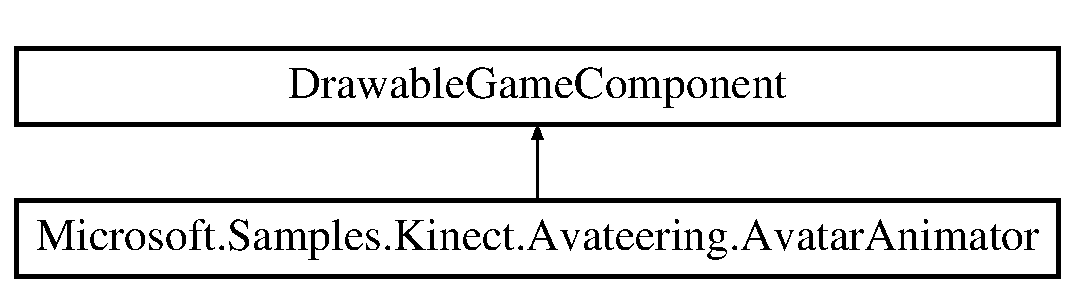
\includegraphics[height=2.000000cm]{class_microsoft_1_1_samples_1_1_kinect_1_1_avateering_1_1_avatar_animator}
\end{center}
\end{figure}
\subsection*{Public Member Functions}
\begin{DoxyCompactItemize}
\item 
\hyperlink{class_microsoft_1_1_samples_1_1_kinect_1_1_avateering_1_1_avatar_animator_a867e1504135b023647dcfe7ccfa8346b}{Avatar\+Animator} (Game game, \hyperlink{namespace_microsoft_1_1_samples_1_1_kinect_1_1_avateering_a2c91e120476e4f1ece17c53d41ff8327}{Retarget\+Matrix\+Hierarchy\+To\+Avatar\+Mesh} retarget, Vector3 skeleton\+Translation\+Scale\+Factor)
\begin{DoxyCompactList}\small\item\em Initializes a new instance of the \hyperlink{class_microsoft_1_1_samples_1_1_kinect_1_1_avateering_1_1_avatar_animator}{Avatar\+Animator} class. \end{DoxyCompactList}\item 
void \hyperlink{class_microsoft_1_1_samples_1_1_kinect_1_1_avateering_1_1_avatar_animator_ad1d121e16db910507be5d999cd6b0408}{Reset} ()
\begin{DoxyCompactList}\small\item\em Reset the tracking filters. \end{DoxyCompactList}\item 
void \hyperlink{class_microsoft_1_1_samples_1_1_kinect_1_1_avateering_1_1_avatar_animator_adb8495bec1c5f70a396db72d94eee599}{Copy\+Skeleton} (Skeleton source\+Skeleton)
\begin{DoxyCompactList}\small\item\em This method copies a new skeleton locally so we can modify it. \end{DoxyCompactList}\item 
override void \hyperlink{class_microsoft_1_1_samples_1_1_kinect_1_1_avateering_1_1_avatar_animator_a46df6cf97a78c7ade81427b77cab321e}{Update} (Game\+Time game\+Time)
\begin{DoxyCompactList}\small\item\em This method retrieves a new skeleton frame if necessary. \end{DoxyCompactList}\item 
void \hyperlink{class_microsoft_1_1_samples_1_1_kinect_1_1_avateering_1_1_avatar_animator_a310a799c7fe1e687ddc27f3b02f1d354}{Draw} (Game\+Time game\+Time, Matrix world, Matrix view, Matrix projection)
\begin{DoxyCompactList}\small\item\em This method draws the skeleton frame data. \end{DoxyCompactList}\end{DoxyCompactItemize}
\subsection*{Properties}
\begin{DoxyCompactItemize}
\item 
bool \hyperlink{class_microsoft_1_1_samples_1_1_kinect_1_1_avateering_1_1_avatar_animator_aac2c33858a422df79802e332db84fcd1}{Skeleton\+Drawn}\hspace{0.3cm}{\ttfamily  \mbox{[}get, set\mbox{]}}
\begin{DoxyCompactList}\small\item\em Gets or sets a value indicating whether the model has been drawn -\/ this flag ensures we only request a frame once per update call across the entire application. \end{DoxyCompactList}\item 
bool \hyperlink{class_microsoft_1_1_samples_1_1_kinect_1_1_avateering_1_1_avatar_animator_a3185fd0fe9fd0db6d0ac75083a490c4c}{Skeleton\+Visible}\hspace{0.3cm}{\ttfamily  \mbox{[}get, set\mbox{]}}
\begin{DoxyCompactList}\small\item\em Gets or sets a value indicating whether this model is visible -\/ this flag ensures we only update if there is visible data. \end{DoxyCompactList}\item 
Skeleton \hyperlink{class_microsoft_1_1_samples_1_1_kinect_1_1_avateering_1_1_avatar_animator_ae4db88033826109723fb2ddf97f1331a}{Raw\+Skeleton}\hspace{0.3cm}{\ttfamily  \mbox{[}get, set\mbox{]}}
\begin{DoxyCompactList}\small\item\em Gets or sets a value indicating whether the first tracked skeleton in the frame is used for animation. \end{DoxyCompactList}\item 
System.\+Tuple$<$ float, float, \\*
float, float $>$ \hyperlink{class_microsoft_1_1_samples_1_1_kinect_1_1_avateering_1_1_avatar_animator_a3f5a9221dc2119e038dca80bae049d8a}{Floor\+Clip\+Plane}\hspace{0.3cm}{\ttfamily  \mbox{[}get, set\mbox{]}}
\begin{DoxyCompactList}\small\item\em Gets or sets a value indicating whether Store the floor plane to compensate the skeletons for any \hyperlink{namespace_microsoft_1_1_samples_1_1_kinect}{Kinect} tilt. \end{DoxyCompactList}\item 
float \hyperlink{class_microsoft_1_1_samples_1_1_kinect_1_1_avateering_1_1_avatar_animator_a0af976059d0d5692d70c7fa6e35c1bd7}{Avatar\+Hip\+Center\+Height}\hspace{0.3cm}{\ttfamily  \mbox{[}get, set\mbox{]}}
\begin{DoxyCompactList}\small\item\em Gets or sets a value indicating whether the height of the avatar Hip Center joint off the floor when standing upright. \end{DoxyCompactList}\item 
\hyperlink{class_microsoft_1_1_samples_1_1_kinect_1_1_avateering_1_1_kinect_chooser}{Kinect\+Chooser} \hyperlink{class_microsoft_1_1_samples_1_1_kinect_1_1_avateering_1_1_avatar_animator_a80c63506559b26d0850796c9563fd449}{Chooser}\hspace{0.3cm}{\ttfamily  \mbox{[}get\mbox{]}}
\begin{DoxyCompactList}\small\item\em Gets the \hyperlink{class_microsoft_1_1_samples_1_1_kinect_1_1_avateering_1_1_kinect_chooser}{Kinect\+Chooser} from the services. \end{DoxyCompactList}\item 
Model \hyperlink{class_microsoft_1_1_samples_1_1_kinect_1_1_avateering_1_1_avatar_animator_a6387822c328c988fe91ce1dacff089b8}{Avatar}\hspace{0.3cm}{\ttfamily  \mbox{[}get, set\mbox{]}}
\begin{DoxyCompactList}\small\item\em Gets or sets the Avatar 3\+D model to animate. \end{DoxyCompactList}\end{DoxyCompactItemize}


\subsection{Detailed Description}
This class is responsible for animating an avatar using a skeleton stream. 



\subsection{Constructor \& Destructor Documentation}
\hypertarget{class_microsoft_1_1_samples_1_1_kinect_1_1_avateering_1_1_avatar_animator_a867e1504135b023647dcfe7ccfa8346b}{\index{Microsoft\+::\+Samples\+::\+Kinect\+::\+Avateering\+::\+Avatar\+Animator@{Microsoft\+::\+Samples\+::\+Kinect\+::\+Avateering\+::\+Avatar\+Animator}!Avatar\+Animator@{Avatar\+Animator}}
\index{Avatar\+Animator@{Avatar\+Animator}!Microsoft\+::\+Samples\+::\+Kinect\+::\+Avateering\+::\+Avatar\+Animator@{Microsoft\+::\+Samples\+::\+Kinect\+::\+Avateering\+::\+Avatar\+Animator}}
\subsubsection[{Avatar\+Animator}]{\setlength{\rightskip}{0pt plus 5cm}Microsoft.\+Samples.\+Kinect.\+Avateering.\+Avatar\+Animator.\+Avatar\+Animator (
\begin{DoxyParamCaption}
\item[{Game}]{game, }
\item[{{\bf Retarget\+Matrix\+Hierarchy\+To\+Avatar\+Mesh}}]{retarget, }
\item[{Vector3}]{skeleton\+Translation\+Scale\+Factor}
\end{DoxyParamCaption}
)}}\label{class_microsoft_1_1_samples_1_1_kinect_1_1_avateering_1_1_avatar_animator_a867e1504135b023647dcfe7ccfa8346b}


Initializes a new instance of the \hyperlink{class_microsoft_1_1_samples_1_1_kinect_1_1_avateering_1_1_avatar_animator}{Avatar\+Animator} class. 


\begin{DoxyParams}{Parameters}
{\em game} & The related game object.\\
\hline
{\em retarget} & The avatar mesh re-\/targeting method to convert from the \hyperlink{namespace_microsoft_1_1_samples_1_1_kinect}{Kinect} skeleton.\\
\hline
\end{DoxyParams}


\subsection{Member Function Documentation}
\hypertarget{class_microsoft_1_1_samples_1_1_kinect_1_1_avateering_1_1_avatar_animator_adb8495bec1c5f70a396db72d94eee599}{\index{Microsoft\+::\+Samples\+::\+Kinect\+::\+Avateering\+::\+Avatar\+Animator@{Microsoft\+::\+Samples\+::\+Kinect\+::\+Avateering\+::\+Avatar\+Animator}!Copy\+Skeleton@{Copy\+Skeleton}}
\index{Copy\+Skeleton@{Copy\+Skeleton}!Microsoft\+::\+Samples\+::\+Kinect\+::\+Avateering\+::\+Avatar\+Animator@{Microsoft\+::\+Samples\+::\+Kinect\+::\+Avateering\+::\+Avatar\+Animator}}
\subsubsection[{Copy\+Skeleton}]{\setlength{\rightskip}{0pt plus 5cm}void Microsoft.\+Samples.\+Kinect.\+Avateering.\+Avatar\+Animator.\+Copy\+Skeleton (
\begin{DoxyParamCaption}
\item[{Skeleton}]{source\+Skeleton}
\end{DoxyParamCaption}
)}}\label{class_microsoft_1_1_samples_1_1_kinect_1_1_avateering_1_1_avatar_animator_adb8495bec1c5f70a396db72d94eee599}


This method copies a new skeleton locally so we can modify it. 


\begin{DoxyParams}{Parameters}
{\em source\+Skeleton} & The skeleton to copy.\\
\hline
\end{DoxyParams}
\hypertarget{class_microsoft_1_1_samples_1_1_kinect_1_1_avateering_1_1_avatar_animator_a310a799c7fe1e687ddc27f3b02f1d354}{\index{Microsoft\+::\+Samples\+::\+Kinect\+::\+Avateering\+::\+Avatar\+Animator@{Microsoft\+::\+Samples\+::\+Kinect\+::\+Avateering\+::\+Avatar\+Animator}!Draw@{Draw}}
\index{Draw@{Draw}!Microsoft\+::\+Samples\+::\+Kinect\+::\+Avateering\+::\+Avatar\+Animator@{Microsoft\+::\+Samples\+::\+Kinect\+::\+Avateering\+::\+Avatar\+Animator}}
\subsubsection[{Draw}]{\setlength{\rightskip}{0pt plus 5cm}void Microsoft.\+Samples.\+Kinect.\+Avateering.\+Avatar\+Animator.\+Draw (
\begin{DoxyParamCaption}
\item[{Game\+Time}]{game\+Time, }
\item[{Matrix}]{world, }
\item[{Matrix}]{view, }
\item[{Matrix}]{projection}
\end{DoxyParamCaption}
)}}\label{class_microsoft_1_1_samples_1_1_kinect_1_1_avateering_1_1_avatar_animator_a310a799c7fe1e687ddc27f3b02f1d354}


This method draws the skeleton frame data. 


\begin{DoxyParams}{Parameters}
{\em game\+Time} & The elapsed game time.\\
\hline
{\em world} & The world matrix.\\
\hline
{\em view} & The view matrix.\\
\hline
{\em projection} & The projection matrix.\\
\hline
\end{DoxyParams}
\hypertarget{class_microsoft_1_1_samples_1_1_kinect_1_1_avateering_1_1_avatar_animator_ad1d121e16db910507be5d999cd6b0408}{\index{Microsoft\+::\+Samples\+::\+Kinect\+::\+Avateering\+::\+Avatar\+Animator@{Microsoft\+::\+Samples\+::\+Kinect\+::\+Avateering\+::\+Avatar\+Animator}!Reset@{Reset}}
\index{Reset@{Reset}!Microsoft\+::\+Samples\+::\+Kinect\+::\+Avateering\+::\+Avatar\+Animator@{Microsoft\+::\+Samples\+::\+Kinect\+::\+Avateering\+::\+Avatar\+Animator}}
\subsubsection[{Reset}]{\setlength{\rightskip}{0pt plus 5cm}void Microsoft.\+Samples.\+Kinect.\+Avateering.\+Avatar\+Animator.\+Reset (
\begin{DoxyParamCaption}
{}
\end{DoxyParamCaption}
)}}\label{class_microsoft_1_1_samples_1_1_kinect_1_1_avateering_1_1_avatar_animator_ad1d121e16db910507be5d999cd6b0408}


Reset the tracking filters. 

\hypertarget{class_microsoft_1_1_samples_1_1_kinect_1_1_avateering_1_1_avatar_animator_a46df6cf97a78c7ade81427b77cab321e}{\index{Microsoft\+::\+Samples\+::\+Kinect\+::\+Avateering\+::\+Avatar\+Animator@{Microsoft\+::\+Samples\+::\+Kinect\+::\+Avateering\+::\+Avatar\+Animator}!Update@{Update}}
\index{Update@{Update}!Microsoft\+::\+Samples\+::\+Kinect\+::\+Avateering\+::\+Avatar\+Animator@{Microsoft\+::\+Samples\+::\+Kinect\+::\+Avateering\+::\+Avatar\+Animator}}
\subsubsection[{Update}]{\setlength{\rightskip}{0pt plus 5cm}override void Microsoft.\+Samples.\+Kinect.\+Avateering.\+Avatar\+Animator.\+Update (
\begin{DoxyParamCaption}
\item[{Game\+Time}]{game\+Time}
\end{DoxyParamCaption}
)}}\label{class_microsoft_1_1_samples_1_1_kinect_1_1_avateering_1_1_avatar_animator_a46df6cf97a78c7ade81427b77cab321e}


This method retrieves a new skeleton frame if necessary. 


\begin{DoxyParams}{Parameters}
{\em game\+Time} & The elapsed game time.\\
\hline
\end{DoxyParams}


\subsection{Property Documentation}
\hypertarget{class_microsoft_1_1_samples_1_1_kinect_1_1_avateering_1_1_avatar_animator_a6387822c328c988fe91ce1dacff089b8}{\index{Microsoft\+::\+Samples\+::\+Kinect\+::\+Avateering\+::\+Avatar\+Animator@{Microsoft\+::\+Samples\+::\+Kinect\+::\+Avateering\+::\+Avatar\+Animator}!Avatar@{Avatar}}
\index{Avatar@{Avatar}!Microsoft\+::\+Samples\+::\+Kinect\+::\+Avateering\+::\+Avatar\+Animator@{Microsoft\+::\+Samples\+::\+Kinect\+::\+Avateering\+::\+Avatar\+Animator}}
\subsubsection[{Avatar}]{\setlength{\rightskip}{0pt plus 5cm}Model Microsoft.\+Samples.\+Kinect.\+Avateering.\+Avatar\+Animator.\+Avatar\hspace{0.3cm}{\ttfamily [get]}, {\ttfamily [set]}}}\label{class_microsoft_1_1_samples_1_1_kinect_1_1_avateering_1_1_avatar_animator_a6387822c328c988fe91ce1dacff089b8}


Gets or sets the Avatar 3\+D model to animate. 

\hypertarget{class_microsoft_1_1_samples_1_1_kinect_1_1_avateering_1_1_avatar_animator_a0af976059d0d5692d70c7fa6e35c1bd7}{\index{Microsoft\+::\+Samples\+::\+Kinect\+::\+Avateering\+::\+Avatar\+Animator@{Microsoft\+::\+Samples\+::\+Kinect\+::\+Avateering\+::\+Avatar\+Animator}!Avatar\+Hip\+Center\+Height@{Avatar\+Hip\+Center\+Height}}
\index{Avatar\+Hip\+Center\+Height@{Avatar\+Hip\+Center\+Height}!Microsoft\+::\+Samples\+::\+Kinect\+::\+Avateering\+::\+Avatar\+Animator@{Microsoft\+::\+Samples\+::\+Kinect\+::\+Avateering\+::\+Avatar\+Animator}}
\subsubsection[{Avatar\+Hip\+Center\+Height}]{\setlength{\rightskip}{0pt plus 5cm}float Microsoft.\+Samples.\+Kinect.\+Avateering.\+Avatar\+Animator.\+Avatar\+Hip\+Center\+Height\hspace{0.3cm}{\ttfamily [get]}, {\ttfamily [set]}}}\label{class_microsoft_1_1_samples_1_1_kinect_1_1_avateering_1_1_avatar_animator_a0af976059d0d5692d70c7fa6e35c1bd7}


Gets or sets a value indicating whether the height of the avatar Hip Center joint off the floor when standing upright. 

\hypertarget{class_microsoft_1_1_samples_1_1_kinect_1_1_avateering_1_1_avatar_animator_a80c63506559b26d0850796c9563fd449}{\index{Microsoft\+::\+Samples\+::\+Kinect\+::\+Avateering\+::\+Avatar\+Animator@{Microsoft\+::\+Samples\+::\+Kinect\+::\+Avateering\+::\+Avatar\+Animator}!Chooser@{Chooser}}
\index{Chooser@{Chooser}!Microsoft\+::\+Samples\+::\+Kinect\+::\+Avateering\+::\+Avatar\+Animator@{Microsoft\+::\+Samples\+::\+Kinect\+::\+Avateering\+::\+Avatar\+Animator}}
\subsubsection[{Chooser}]{\setlength{\rightskip}{0pt plus 5cm}{\bf Kinect\+Chooser} Microsoft.\+Samples.\+Kinect.\+Avateering.\+Avatar\+Animator.\+Chooser\hspace{0.3cm}{\ttfamily [get]}}}\label{class_microsoft_1_1_samples_1_1_kinect_1_1_avateering_1_1_avatar_animator_a80c63506559b26d0850796c9563fd449}


Gets the \hyperlink{class_microsoft_1_1_samples_1_1_kinect_1_1_avateering_1_1_kinect_chooser}{Kinect\+Chooser} from the services. 

\hypertarget{class_microsoft_1_1_samples_1_1_kinect_1_1_avateering_1_1_avatar_animator_a3f5a9221dc2119e038dca80bae049d8a}{\index{Microsoft\+::\+Samples\+::\+Kinect\+::\+Avateering\+::\+Avatar\+Animator@{Microsoft\+::\+Samples\+::\+Kinect\+::\+Avateering\+::\+Avatar\+Animator}!Floor\+Clip\+Plane@{Floor\+Clip\+Plane}}
\index{Floor\+Clip\+Plane@{Floor\+Clip\+Plane}!Microsoft\+::\+Samples\+::\+Kinect\+::\+Avateering\+::\+Avatar\+Animator@{Microsoft\+::\+Samples\+::\+Kinect\+::\+Avateering\+::\+Avatar\+Animator}}
\subsubsection[{Floor\+Clip\+Plane}]{\setlength{\rightskip}{0pt plus 5cm}System.\+Tuple$<$float, float, float, float$>$ Microsoft.\+Samples.\+Kinect.\+Avateering.\+Avatar\+Animator.\+Floor\+Clip\+Plane\hspace{0.3cm}{\ttfamily [get]}, {\ttfamily [set]}}}\label{class_microsoft_1_1_samples_1_1_kinect_1_1_avateering_1_1_avatar_animator_a3f5a9221dc2119e038dca80bae049d8a}


Gets or sets a value indicating whether Store the floor plane to compensate the skeletons for any \hyperlink{namespace_microsoft_1_1_samples_1_1_kinect}{Kinect} tilt. 

\hypertarget{class_microsoft_1_1_samples_1_1_kinect_1_1_avateering_1_1_avatar_animator_ae4db88033826109723fb2ddf97f1331a}{\index{Microsoft\+::\+Samples\+::\+Kinect\+::\+Avateering\+::\+Avatar\+Animator@{Microsoft\+::\+Samples\+::\+Kinect\+::\+Avateering\+::\+Avatar\+Animator}!Raw\+Skeleton@{Raw\+Skeleton}}
\index{Raw\+Skeleton@{Raw\+Skeleton}!Microsoft\+::\+Samples\+::\+Kinect\+::\+Avateering\+::\+Avatar\+Animator@{Microsoft\+::\+Samples\+::\+Kinect\+::\+Avateering\+::\+Avatar\+Animator}}
\subsubsection[{Raw\+Skeleton}]{\setlength{\rightskip}{0pt plus 5cm}Skeleton Microsoft.\+Samples.\+Kinect.\+Avateering.\+Avatar\+Animator.\+Raw\+Skeleton\hspace{0.3cm}{\ttfamily [get]}, {\ttfamily [set]}}}\label{class_microsoft_1_1_samples_1_1_kinect_1_1_avateering_1_1_avatar_animator_ae4db88033826109723fb2ddf97f1331a}


Gets or sets a value indicating whether the first tracked skeleton in the frame is used for animation. 

\hypertarget{class_microsoft_1_1_samples_1_1_kinect_1_1_avateering_1_1_avatar_animator_aac2c33858a422df79802e332db84fcd1}{\index{Microsoft\+::\+Samples\+::\+Kinect\+::\+Avateering\+::\+Avatar\+Animator@{Microsoft\+::\+Samples\+::\+Kinect\+::\+Avateering\+::\+Avatar\+Animator}!Skeleton\+Drawn@{Skeleton\+Drawn}}
\index{Skeleton\+Drawn@{Skeleton\+Drawn}!Microsoft\+::\+Samples\+::\+Kinect\+::\+Avateering\+::\+Avatar\+Animator@{Microsoft\+::\+Samples\+::\+Kinect\+::\+Avateering\+::\+Avatar\+Animator}}
\subsubsection[{Skeleton\+Drawn}]{\setlength{\rightskip}{0pt plus 5cm}bool Microsoft.\+Samples.\+Kinect.\+Avateering.\+Avatar\+Animator.\+Skeleton\+Drawn\hspace{0.3cm}{\ttfamily [get]}, {\ttfamily [set]}}}\label{class_microsoft_1_1_samples_1_1_kinect_1_1_avateering_1_1_avatar_animator_aac2c33858a422df79802e332db84fcd1}


Gets or sets a value indicating whether the model has been drawn -\/ this flag ensures we only request a frame once per update call across the entire application. 

\hypertarget{class_microsoft_1_1_samples_1_1_kinect_1_1_avateering_1_1_avatar_animator_a3185fd0fe9fd0db6d0ac75083a490c4c}{\index{Microsoft\+::\+Samples\+::\+Kinect\+::\+Avateering\+::\+Avatar\+Animator@{Microsoft\+::\+Samples\+::\+Kinect\+::\+Avateering\+::\+Avatar\+Animator}!Skeleton\+Visible@{Skeleton\+Visible}}
\index{Skeleton\+Visible@{Skeleton\+Visible}!Microsoft\+::\+Samples\+::\+Kinect\+::\+Avateering\+::\+Avatar\+Animator@{Microsoft\+::\+Samples\+::\+Kinect\+::\+Avateering\+::\+Avatar\+Animator}}
\subsubsection[{Skeleton\+Visible}]{\setlength{\rightskip}{0pt plus 5cm}bool Microsoft.\+Samples.\+Kinect.\+Avateering.\+Avatar\+Animator.\+Skeleton\+Visible\hspace{0.3cm}{\ttfamily [get]}, {\ttfamily [set]}}}\label{class_microsoft_1_1_samples_1_1_kinect_1_1_avateering_1_1_avatar_animator_a3185fd0fe9fd0db6d0ac75083a490c4c}


Gets or sets a value indicating whether this model is visible -\/ this flag ensures we only update if there is visible data. 



The documentation for this class was generated from the following file\+:\begin{DoxyCompactItemize}
\item 
Avateering/Avatar\+Animator.\+cs\end{DoxyCompactItemize}

\hypertarget{class_microsoft_1_1_samples_1_1_kinect_1_1_avateering_1_1_avateering_x_n_a}{\section{Microsoft.\+Samples.\+Kinect.\+Avateering.\+Avateering\+X\+N\+A Class Reference}
\label{class_microsoft_1_1_samples_1_1_kinect_1_1_avateering_1_1_avateering_x_n_a}\index{Microsoft.\+Samples.\+Kinect.\+Avateering.\+Avateering\+X\+N\+A@{Microsoft.\+Samples.\+Kinect.\+Avateering.\+Avateering\+X\+N\+A}}
}


Ce programme permet de porter virtuellement des v�tements en 3\+D  


Inheritance diagram for Microsoft.\+Samples.\+Kinect.\+Avateering.\+Avateering\+X\+N\+A\+:\begin{figure}[H]
\begin{center}
\leavevmode
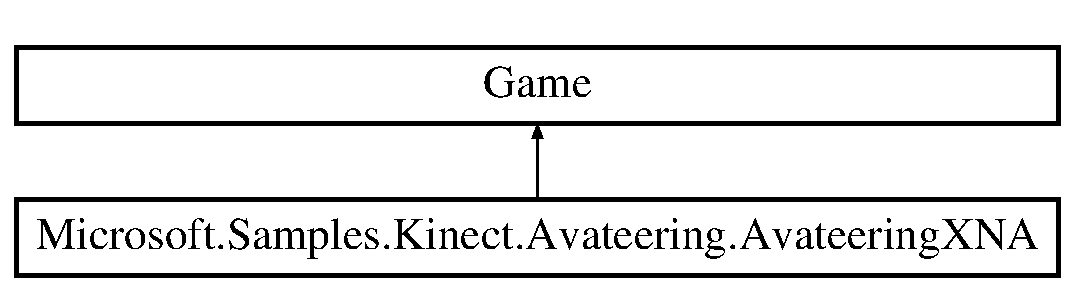
\includegraphics[height=2.000000cm]{class_microsoft_1_1_samples_1_1_kinect_1_1_avateering_1_1_avateering_x_n_a}
\end{center}
\end{figure}
\subsection*{Public Member Functions}
\begin{DoxyCompactItemize}
\item 
\hyperlink{class_microsoft_1_1_samples_1_1_kinect_1_1_avateering_1_1_avateering_x_n_a_a4671fd4278d311bbdfa9e89eaf0da466}{Avateering\+X\+N\+A} ()
\begin{DoxyCompactList}\small\item\em Initializes une nouvelle instance de la classe \hyperlink{class_microsoft_1_1_samples_1_1_kinect_1_1_avateering_1_1_avateering_x_n_a}{Avateering\+X\+N\+A}. \end{DoxyCompactList}\end{DoxyCompactItemize}
\subsection*{Protected Member Functions}
\begin{DoxyCompactItemize}
\item 
override void \hyperlink{class_microsoft_1_1_samples_1_1_kinect_1_1_avateering_1_1_avateering_x_n_a_a88421d7d7bbf6828622cf925e1e32ea1}{Load\+Content} ()
\begin{DoxyCompactList}\small\item\em Charge le contenu graphique. \end{DoxyCompactList}\item 
void \hyperlink{class_microsoft_1_1_samples_1_1_kinect_1_1_avateering_1_1_avateering_x_n_a_a24e68729f42a908ed2880d5ab4b205e0}{Build\+Joint\+Hierarchy} ()
\begin{DoxyCompactList}\small\item\em Cette fonction fait l'�quivalence entre le squelette de la kinect et le squelette du mod�le \end{DoxyCompactList}\item 
override void \hyperlink{class_microsoft_1_1_samples_1_1_kinect_1_1_avateering_1_1_avateering_x_n_a_a2dd0406dfab788b9e2275e7a01f23cf2}{Update} (Game\+Time game\+Time)
\begin{DoxyCompactList}\small\item\em Permet au jeu de fonctionner. \end{DoxyCompactList}\item 
void \hyperlink{class_microsoft_1_1_samples_1_1_kinect_1_1_avateering_1_1_avateering_x_n_a_a581371472069c4ec3d8579acb0f435de}{Update\+Viewing\+Camera} ()
\begin{DoxyCompactList}\small\item\em Cr�e la camera \end{DoxyCompactList}\item 
override void \hyperlink{class_microsoft_1_1_samples_1_1_kinect_1_1_avateering_1_1_avateering_x_n_a_a4c79b13871acaa204e56d9f8e7cdf781}{Draw} (Game\+Time game\+Time)
\begin{DoxyCompactList}\small\item\em Cette m�thode renvoit l'�tat en cours \end{DoxyCompactList}\end{DoxyCompactItemize}
\subsection*{Properties}
\begin{DoxyCompactItemize}
\item 
\hyperlink{class_microsoft_1_1_samples_1_1_kinect_1_1_avateering_1_1_kinect_chooser}{Kinect\+Chooser} \hyperlink{class_microsoft_1_1_samples_1_1_kinect_1_1_avateering_1_1_avateering_x_n_a_a13ef43c29e79b980dc9c13db83af13a5}{Chooser}\hspace{0.3cm}{\ttfamily  \mbox{[}get\mbox{]}}
\begin{DoxyCompactList}\small\item\em Obtient le \hyperlink{class_microsoft_1_1_samples_1_1_kinect_1_1_avateering_1_1_kinect_chooser}{Kinect\+Chooser}. \end{DoxyCompactList}\item 
Sprite\+Batch \hyperlink{class_microsoft_1_1_samples_1_1_kinect_1_1_avateering_1_1_avateering_x_n_a_add0fab2901a2aaef868a455f466970ab}{Shared\+Sprite\+Batch}\hspace{0.3cm}{\ttfamily  \mbox{[}get\mbox{]}}
\begin{DoxyCompactList}\small\item\em Obtient le Sprite\+Batch. \end{DoxyCompactList}\end{DoxyCompactItemize}


\subsection{Detailed Description}
Ce programme permet de porter virtuellement des v�tements en 3\+D 



\subsection{Constructor \& Destructor Documentation}
\hypertarget{class_microsoft_1_1_samples_1_1_kinect_1_1_avateering_1_1_avateering_x_n_a_a4671fd4278d311bbdfa9e89eaf0da466}{\index{Microsoft\+::\+Samples\+::\+Kinect\+::\+Avateering\+::\+Avateering\+X\+N\+A@{Microsoft\+::\+Samples\+::\+Kinect\+::\+Avateering\+::\+Avateering\+X\+N\+A}!Avateering\+X\+N\+A@{Avateering\+X\+N\+A}}
\index{Avateering\+X\+N\+A@{Avateering\+X\+N\+A}!Microsoft\+::\+Samples\+::\+Kinect\+::\+Avateering\+::\+Avateering\+X\+N\+A@{Microsoft\+::\+Samples\+::\+Kinect\+::\+Avateering\+::\+Avateering\+X\+N\+A}}
\subsubsection[{Avateering\+X\+N\+A}]{\setlength{\rightskip}{0pt plus 5cm}Microsoft.\+Samples.\+Kinect.\+Avateering.\+Avateering\+X\+N\+A.\+Avateering\+X\+N\+A (
\begin{DoxyParamCaption}
{}
\end{DoxyParamCaption}
)}}\label{class_microsoft_1_1_samples_1_1_kinect_1_1_avateering_1_1_avateering_x_n_a_a4671fd4278d311bbdfa9e89eaf0da466}


Initializes une nouvelle instance de la classe \hyperlink{class_microsoft_1_1_samples_1_1_kinect_1_1_avateering_1_1_avateering_x_n_a}{Avateering\+X\+N\+A}. 



\subsection{Member Function Documentation}
\hypertarget{class_microsoft_1_1_samples_1_1_kinect_1_1_avateering_1_1_avateering_x_n_a_a24e68729f42a908ed2880d5ab4b205e0}{\index{Microsoft\+::\+Samples\+::\+Kinect\+::\+Avateering\+::\+Avateering\+X\+N\+A@{Microsoft\+::\+Samples\+::\+Kinect\+::\+Avateering\+::\+Avateering\+X\+N\+A}!Build\+Joint\+Hierarchy@{Build\+Joint\+Hierarchy}}
\index{Build\+Joint\+Hierarchy@{Build\+Joint\+Hierarchy}!Microsoft\+::\+Samples\+::\+Kinect\+::\+Avateering\+::\+Avateering\+X\+N\+A@{Microsoft\+::\+Samples\+::\+Kinect\+::\+Avateering\+::\+Avateering\+X\+N\+A}}
\subsubsection[{Build\+Joint\+Hierarchy}]{\setlength{\rightskip}{0pt plus 5cm}void Microsoft.\+Samples.\+Kinect.\+Avateering.\+Avateering\+X\+N\+A.\+Build\+Joint\+Hierarchy (
\begin{DoxyParamCaption}
{}
\end{DoxyParamCaption}
)\hspace{0.3cm}{\ttfamily [protected]}}}\label{class_microsoft_1_1_samples_1_1_kinect_1_1_avateering_1_1_avateering_x_n_a_a24e68729f42a908ed2880d5ab4b205e0}


Cette fonction fait l'�quivalence entre le squelette de la kinect et le squelette du mod�le 

\hypertarget{class_microsoft_1_1_samples_1_1_kinect_1_1_avateering_1_1_avateering_x_n_a_a4c79b13871acaa204e56d9f8e7cdf781}{\index{Microsoft\+::\+Samples\+::\+Kinect\+::\+Avateering\+::\+Avateering\+X\+N\+A@{Microsoft\+::\+Samples\+::\+Kinect\+::\+Avateering\+::\+Avateering\+X\+N\+A}!Draw@{Draw}}
\index{Draw@{Draw}!Microsoft\+::\+Samples\+::\+Kinect\+::\+Avateering\+::\+Avateering\+X\+N\+A@{Microsoft\+::\+Samples\+::\+Kinect\+::\+Avateering\+::\+Avateering\+X\+N\+A}}
\subsubsection[{Draw}]{\setlength{\rightskip}{0pt plus 5cm}override void Microsoft.\+Samples.\+Kinect.\+Avateering.\+Avateering\+X\+N\+A.\+Draw (
\begin{DoxyParamCaption}
\item[{Game\+Time}]{game\+Time}
\end{DoxyParamCaption}
)\hspace{0.3cm}{\ttfamily [protected]}}}\label{class_microsoft_1_1_samples_1_1_kinect_1_1_avateering_1_1_avateering_x_n_a_a4c79b13871acaa204e56d9f8e7cdf781}


Cette m�thode renvoit l'�tat en cours 


\begin{DoxyParams}{Parameters}
{\em game\+Time} & The elapsed game time.\\
\hline
\end{DoxyParams}
\hypertarget{class_microsoft_1_1_samples_1_1_kinect_1_1_avateering_1_1_avateering_x_n_a_a88421d7d7bbf6828622cf925e1e32ea1}{\index{Microsoft\+::\+Samples\+::\+Kinect\+::\+Avateering\+::\+Avateering\+X\+N\+A@{Microsoft\+::\+Samples\+::\+Kinect\+::\+Avateering\+::\+Avateering\+X\+N\+A}!Load\+Content@{Load\+Content}}
\index{Load\+Content@{Load\+Content}!Microsoft\+::\+Samples\+::\+Kinect\+::\+Avateering\+::\+Avateering\+X\+N\+A@{Microsoft\+::\+Samples\+::\+Kinect\+::\+Avateering\+::\+Avateering\+X\+N\+A}}
\subsubsection[{Load\+Content}]{\setlength{\rightskip}{0pt plus 5cm}override void Microsoft.\+Samples.\+Kinect.\+Avateering.\+Avateering\+X\+N\+A.\+Load\+Content (
\begin{DoxyParamCaption}
{}
\end{DoxyParamCaption}
)\hspace{0.3cm}{\ttfamily [protected]}}}\label{class_microsoft_1_1_samples_1_1_kinect_1_1_avateering_1_1_avateering_x_n_a_a88421d7d7bbf6828622cf925e1e32ea1}


Charge le contenu graphique. 

\hypertarget{class_microsoft_1_1_samples_1_1_kinect_1_1_avateering_1_1_avateering_x_n_a_a2dd0406dfab788b9e2275e7a01f23cf2}{\index{Microsoft\+::\+Samples\+::\+Kinect\+::\+Avateering\+::\+Avateering\+X\+N\+A@{Microsoft\+::\+Samples\+::\+Kinect\+::\+Avateering\+::\+Avateering\+X\+N\+A}!Update@{Update}}
\index{Update@{Update}!Microsoft\+::\+Samples\+::\+Kinect\+::\+Avateering\+::\+Avateering\+X\+N\+A@{Microsoft\+::\+Samples\+::\+Kinect\+::\+Avateering\+::\+Avateering\+X\+N\+A}}
\subsubsection[{Update}]{\setlength{\rightskip}{0pt plus 5cm}override void Microsoft.\+Samples.\+Kinect.\+Avateering.\+Avateering\+X\+N\+A.\+Update (
\begin{DoxyParamCaption}
\item[{Game\+Time}]{game\+Time}
\end{DoxyParamCaption}
)\hspace{0.3cm}{\ttfamily [protected]}}}\label{class_microsoft_1_1_samples_1_1_kinect_1_1_avateering_1_1_avateering_x_n_a_a2dd0406dfab788b9e2275e7a01f23cf2}


Permet au jeu de fonctionner. 


\begin{DoxyParams}{Parameters}
{\em game\+Time} & The gametime.\\
\hline
\end{DoxyParams}
\hypertarget{class_microsoft_1_1_samples_1_1_kinect_1_1_avateering_1_1_avateering_x_n_a_a581371472069c4ec3d8579acb0f435de}{\index{Microsoft\+::\+Samples\+::\+Kinect\+::\+Avateering\+::\+Avateering\+X\+N\+A@{Microsoft\+::\+Samples\+::\+Kinect\+::\+Avateering\+::\+Avateering\+X\+N\+A}!Update\+Viewing\+Camera@{Update\+Viewing\+Camera}}
\index{Update\+Viewing\+Camera@{Update\+Viewing\+Camera}!Microsoft\+::\+Samples\+::\+Kinect\+::\+Avateering\+::\+Avateering\+X\+N\+A@{Microsoft\+::\+Samples\+::\+Kinect\+::\+Avateering\+::\+Avateering\+X\+N\+A}}
\subsubsection[{Update\+Viewing\+Camera}]{\setlength{\rightskip}{0pt plus 5cm}void Microsoft.\+Samples.\+Kinect.\+Avateering.\+Avateering\+X\+N\+A.\+Update\+Viewing\+Camera (
\begin{DoxyParamCaption}
{}
\end{DoxyParamCaption}
)\hspace{0.3cm}{\ttfamily [protected]}}}\label{class_microsoft_1_1_samples_1_1_kinect_1_1_avateering_1_1_avateering_x_n_a_a581371472069c4ec3d8579acb0f435de}


Cr�e la camera 



\subsection{Property Documentation}
\hypertarget{class_microsoft_1_1_samples_1_1_kinect_1_1_avateering_1_1_avateering_x_n_a_a13ef43c29e79b980dc9c13db83af13a5}{\index{Microsoft\+::\+Samples\+::\+Kinect\+::\+Avateering\+::\+Avateering\+X\+N\+A@{Microsoft\+::\+Samples\+::\+Kinect\+::\+Avateering\+::\+Avateering\+X\+N\+A}!Chooser@{Chooser}}
\index{Chooser@{Chooser}!Microsoft\+::\+Samples\+::\+Kinect\+::\+Avateering\+::\+Avateering\+X\+N\+A@{Microsoft\+::\+Samples\+::\+Kinect\+::\+Avateering\+::\+Avateering\+X\+N\+A}}
\subsubsection[{Chooser}]{\setlength{\rightskip}{0pt plus 5cm}{\bf Kinect\+Chooser} Microsoft.\+Samples.\+Kinect.\+Avateering.\+Avateering\+X\+N\+A.\+Chooser\hspace{0.3cm}{\ttfamily [get]}}}\label{class_microsoft_1_1_samples_1_1_kinect_1_1_avateering_1_1_avateering_x_n_a_a13ef43c29e79b980dc9c13db83af13a5}


Obtient le \hyperlink{class_microsoft_1_1_samples_1_1_kinect_1_1_avateering_1_1_kinect_chooser}{Kinect\+Chooser}. 

\hypertarget{class_microsoft_1_1_samples_1_1_kinect_1_1_avateering_1_1_avateering_x_n_a_add0fab2901a2aaef868a455f466970ab}{\index{Microsoft\+::\+Samples\+::\+Kinect\+::\+Avateering\+::\+Avateering\+X\+N\+A@{Microsoft\+::\+Samples\+::\+Kinect\+::\+Avateering\+::\+Avateering\+X\+N\+A}!Shared\+Sprite\+Batch@{Shared\+Sprite\+Batch}}
\index{Shared\+Sprite\+Batch@{Shared\+Sprite\+Batch}!Microsoft\+::\+Samples\+::\+Kinect\+::\+Avateering\+::\+Avateering\+X\+N\+A@{Microsoft\+::\+Samples\+::\+Kinect\+::\+Avateering\+::\+Avateering\+X\+N\+A}}
\subsubsection[{Shared\+Sprite\+Batch}]{\setlength{\rightskip}{0pt plus 5cm}Sprite\+Batch Microsoft.\+Samples.\+Kinect.\+Avateering.\+Avateering\+X\+N\+A.\+Shared\+Sprite\+Batch\hspace{0.3cm}{\ttfamily [get]}}}\label{class_microsoft_1_1_samples_1_1_kinect_1_1_avateering_1_1_avateering_x_n_a_add0fab2901a2aaef868a455f466970ab}


Obtient le Sprite\+Batch. 



The documentation for this class was generated from the following file\+:\begin{DoxyCompactItemize}
\item 
Avateering/Avateering\+X\+N\+A.\+cs\end{DoxyCompactItemize}

\hypertarget{class_microsoft_1_1_samples_1_1_kinect_1_1_avateering_1_1_filters_1_1_bone_orientation_constraints}{\section{Microsoft.\+Samples.\+Kinect.\+Avateering.\+Filters.\+Bone\+Orientation\+Constraints Class Reference}
\label{class_microsoft_1_1_samples_1_1_kinect_1_1_avateering_1_1_filters_1_1_bone_orientation_constraints}\index{Microsoft.\+Samples.\+Kinect.\+Avateering.\+Filters.\+Bone\+Orientation\+Constraints@{Microsoft.\+Samples.\+Kinect.\+Avateering.\+Filters.\+Bone\+Orientation\+Constraints}}
}


Filter to correct the joint locations and joint orientations to constraint to range of viable human motion.  


Inheritance diagram for Microsoft.\+Samples.\+Kinect.\+Avateering.\+Filters.\+Bone\+Orientation\+Constraints\+:\begin{figure}[H]
\begin{center}
\leavevmode
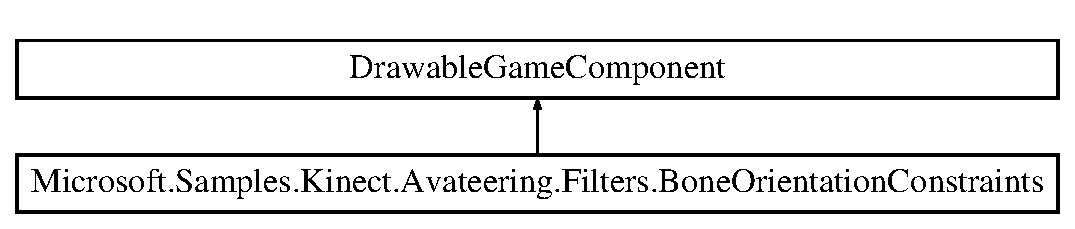
\includegraphics[height=2.000000cm]{class_microsoft_1_1_samples_1_1_kinect_1_1_avateering_1_1_filters_1_1_bone_orientation_constraints}
\end{center}
\end{figure}
\subsection*{Public Member Functions}
\begin{DoxyCompactItemize}
\item 
\hyperlink{class_microsoft_1_1_samples_1_1_kinect_1_1_avateering_1_1_filters_1_1_bone_orientation_constraints_a465df7ac1591095215188b055402e904}{Bone\+Orientation\+Constraints} (Game game, Vector3 skeleton\+Translation\+Scale\+Factor)
\begin{DoxyCompactList}\small\item\em Initializes a new instance of the \hyperlink{class_microsoft_1_1_samples_1_1_kinect_1_1_avateering_1_1_filters_1_1_bone_orientation_constraints}{Bone\+Orientation\+Constraints} class. \end{DoxyCompactList}\item 
void \hyperlink{class_microsoft_1_1_samples_1_1_kinect_1_1_avateering_1_1_filters_1_1_bone_orientation_constraints_aa7de250ad471493e2c5122be569332bf}{Add\+Bone\+Orientation\+Constraint} (Joint\+Type joint, Vector3 dir, float angle)
\begin{DoxyCompactList}\small\item\em Add\+Joint\+Constraint -\/ Adds a joint constraint to the system. \end{DoxyCompactList}\item 
void \hyperlink{class_microsoft_1_1_samples_1_1_kinect_1_1_avateering_1_1_filters_1_1_bone_orientation_constraints_a765f01d12d283f765257f34ef606b812}{Add\+Default\+Constraints} ()
\begin{DoxyCompactList}\small\item\em Add\+Default\+Constraints -\/ Adds a set of default joint constraints for normal human poses. This is a reasonable set of constraints for plausible human bio-\/mechanics. \end{DoxyCompactList}\item 
void \hyperlink{class_microsoft_1_1_samples_1_1_kinect_1_1_avateering_1_1_filters_1_1_bone_orientation_constraints_ac5ad273f2b1ee5a6fafef733290ce114}{Constrain} (Skeleton skeleton, bool mirror\+View)
\begin{DoxyCompactList}\small\item\em Apply\+Bone\+Orientation\+Constraints and constrain rotations. \end{DoxyCompactList}\item 
void \hyperlink{class_microsoft_1_1_samples_1_1_kinect_1_1_avateering_1_1_filters_1_1_bone_orientation_constraints_aecf019a3f152a6b4cdfb6d4f12e6c08c}{Draw} (Game\+Time game\+Time, Skeleton skeleton, bool seated\+Mode, Matrix world, Matrix view, Matrix projection)
\begin{DoxyCompactList}\small\item\em This method draws the skeleton frame data. \end{DoxyCompactList}\end{DoxyCompactItemize}
\subsection*{Protected Member Functions}
\begin{DoxyCompactItemize}
\item 
override void \hyperlink{class_microsoft_1_1_samples_1_1_kinect_1_1_avateering_1_1_filters_1_1_bone_orientation_constraints_a1bb46b424bb16f4839ae25cdc80bbad9}{Load\+Content} ()
\begin{DoxyCompactList}\small\item\em This method loads the avatar model mesh and sets the bind pose. \end{DoxyCompactList}\end{DoxyCompactItemize}


\subsection{Detailed Description}
Filter to correct the joint locations and joint orientations to constraint to range of viable human motion. 



\subsection{Constructor \& Destructor Documentation}
\hypertarget{class_microsoft_1_1_samples_1_1_kinect_1_1_avateering_1_1_filters_1_1_bone_orientation_constraints_a465df7ac1591095215188b055402e904}{\index{Microsoft\+::\+Samples\+::\+Kinect\+::\+Avateering\+::\+Filters\+::\+Bone\+Orientation\+Constraints@{Microsoft\+::\+Samples\+::\+Kinect\+::\+Avateering\+::\+Filters\+::\+Bone\+Orientation\+Constraints}!Bone\+Orientation\+Constraints@{Bone\+Orientation\+Constraints}}
\index{Bone\+Orientation\+Constraints@{Bone\+Orientation\+Constraints}!Microsoft\+::\+Samples\+::\+Kinect\+::\+Avateering\+::\+Filters\+::\+Bone\+Orientation\+Constraints@{Microsoft\+::\+Samples\+::\+Kinect\+::\+Avateering\+::\+Filters\+::\+Bone\+Orientation\+Constraints}}
\subsubsection[{Bone\+Orientation\+Constraints}]{\setlength{\rightskip}{0pt plus 5cm}Microsoft.\+Samples.\+Kinect.\+Avateering.\+Filters.\+Bone\+Orientation\+Constraints.\+Bone\+Orientation\+Constraints (
\begin{DoxyParamCaption}
\item[{Game}]{game, }
\item[{Vector3}]{skeleton\+Translation\+Scale\+Factor}
\end{DoxyParamCaption}
)}}\label{class_microsoft_1_1_samples_1_1_kinect_1_1_avateering_1_1_filters_1_1_bone_orientation_constraints_a465df7ac1591095215188b055402e904}


Initializes a new instance of the \hyperlink{class_microsoft_1_1_samples_1_1_kinect_1_1_avateering_1_1_filters_1_1_bone_orientation_constraints}{Bone\+Orientation\+Constraints} class. 


\begin{DoxyParams}{Parameters}
{\em game} & The related game object.\\
\hline
\end{DoxyParams}


\subsection{Member Function Documentation}
\hypertarget{class_microsoft_1_1_samples_1_1_kinect_1_1_avateering_1_1_filters_1_1_bone_orientation_constraints_aa7de250ad471493e2c5122be569332bf}{\index{Microsoft\+::\+Samples\+::\+Kinect\+::\+Avateering\+::\+Filters\+::\+Bone\+Orientation\+Constraints@{Microsoft\+::\+Samples\+::\+Kinect\+::\+Avateering\+::\+Filters\+::\+Bone\+Orientation\+Constraints}!Add\+Bone\+Orientation\+Constraint@{Add\+Bone\+Orientation\+Constraint}}
\index{Add\+Bone\+Orientation\+Constraint@{Add\+Bone\+Orientation\+Constraint}!Microsoft\+::\+Samples\+::\+Kinect\+::\+Avateering\+::\+Filters\+::\+Bone\+Orientation\+Constraints@{Microsoft\+::\+Samples\+::\+Kinect\+::\+Avateering\+::\+Filters\+::\+Bone\+Orientation\+Constraints}}
\subsubsection[{Add\+Bone\+Orientation\+Constraint}]{\setlength{\rightskip}{0pt plus 5cm}void Microsoft.\+Samples.\+Kinect.\+Avateering.\+Filters.\+Bone\+Orientation\+Constraints.\+Add\+Bone\+Orientation\+Constraint (
\begin{DoxyParamCaption}
\item[{Joint\+Type}]{joint, }
\item[{Vector3}]{dir, }
\item[{float}]{angle}
\end{DoxyParamCaption}
)}}\label{class_microsoft_1_1_samples_1_1_kinect_1_1_avateering_1_1_filters_1_1_bone_orientation_constraints_aa7de250ad471493e2c5122be569332bf}


Add\+Joint\+Constraint -\/ Adds a joint constraint to the system. 


\begin{DoxyParams}{Parameters}
{\em joint} & The skeleton joint/bone.\\
\hline
{\em dir} & The absolute dir for the center of the constraint cone.\\
\hline
{\em angle} & The angle of the constraint cone that the bone can move in.\\
\hline
\end{DoxyParams}
\hypertarget{class_microsoft_1_1_samples_1_1_kinect_1_1_avateering_1_1_filters_1_1_bone_orientation_constraints_a765f01d12d283f765257f34ef606b812}{\index{Microsoft\+::\+Samples\+::\+Kinect\+::\+Avateering\+::\+Filters\+::\+Bone\+Orientation\+Constraints@{Microsoft\+::\+Samples\+::\+Kinect\+::\+Avateering\+::\+Filters\+::\+Bone\+Orientation\+Constraints}!Add\+Default\+Constraints@{Add\+Default\+Constraints}}
\index{Add\+Default\+Constraints@{Add\+Default\+Constraints}!Microsoft\+::\+Samples\+::\+Kinect\+::\+Avateering\+::\+Filters\+::\+Bone\+Orientation\+Constraints@{Microsoft\+::\+Samples\+::\+Kinect\+::\+Avateering\+::\+Filters\+::\+Bone\+Orientation\+Constraints}}
\subsubsection[{Add\+Default\+Constraints}]{\setlength{\rightskip}{0pt plus 5cm}void Microsoft.\+Samples.\+Kinect.\+Avateering.\+Filters.\+Bone\+Orientation\+Constraints.\+Add\+Default\+Constraints (
\begin{DoxyParamCaption}
{}
\end{DoxyParamCaption}
)}}\label{class_microsoft_1_1_samples_1_1_kinect_1_1_avateering_1_1_filters_1_1_bone_orientation_constraints_a765f01d12d283f765257f34ef606b812}


Add\+Default\+Constraints -\/ Adds a set of default joint constraints for normal human poses. This is a reasonable set of constraints for plausible human bio-\/mechanics. 

\hypertarget{class_microsoft_1_1_samples_1_1_kinect_1_1_avateering_1_1_filters_1_1_bone_orientation_constraints_ac5ad273f2b1ee5a6fafef733290ce114}{\index{Microsoft\+::\+Samples\+::\+Kinect\+::\+Avateering\+::\+Filters\+::\+Bone\+Orientation\+Constraints@{Microsoft\+::\+Samples\+::\+Kinect\+::\+Avateering\+::\+Filters\+::\+Bone\+Orientation\+Constraints}!Constrain@{Constrain}}
\index{Constrain@{Constrain}!Microsoft\+::\+Samples\+::\+Kinect\+::\+Avateering\+::\+Filters\+::\+Bone\+Orientation\+Constraints@{Microsoft\+::\+Samples\+::\+Kinect\+::\+Avateering\+::\+Filters\+::\+Bone\+Orientation\+Constraints}}
\subsubsection[{Constrain}]{\setlength{\rightskip}{0pt plus 5cm}void Microsoft.\+Samples.\+Kinect.\+Avateering.\+Filters.\+Bone\+Orientation\+Constraints.\+Constrain (
\begin{DoxyParamCaption}
\item[{Skeleton}]{skeleton, }
\item[{bool}]{mirror\+View}
\end{DoxyParamCaption}
)}}\label{class_microsoft_1_1_samples_1_1_kinect_1_1_avateering_1_1_filters_1_1_bone_orientation_constraints_ac5ad273f2b1ee5a6fafef733290ce114}


Apply\+Bone\+Orientation\+Constraints and constrain rotations. 


\begin{DoxyParams}{Parameters}
{\em skeleton} & The skeleton to correct.\\
\hline
{\em mirror\+View} & Set this true if the skeleton joints are mirrored.\\
\hline
\end{DoxyParams}
\hypertarget{class_microsoft_1_1_samples_1_1_kinect_1_1_avateering_1_1_filters_1_1_bone_orientation_constraints_aecf019a3f152a6b4cdfb6d4f12e6c08c}{\index{Microsoft\+::\+Samples\+::\+Kinect\+::\+Avateering\+::\+Filters\+::\+Bone\+Orientation\+Constraints@{Microsoft\+::\+Samples\+::\+Kinect\+::\+Avateering\+::\+Filters\+::\+Bone\+Orientation\+Constraints}!Draw@{Draw}}
\index{Draw@{Draw}!Microsoft\+::\+Samples\+::\+Kinect\+::\+Avateering\+::\+Filters\+::\+Bone\+Orientation\+Constraints@{Microsoft\+::\+Samples\+::\+Kinect\+::\+Avateering\+::\+Filters\+::\+Bone\+Orientation\+Constraints}}
\subsubsection[{Draw}]{\setlength{\rightskip}{0pt plus 5cm}void Microsoft.\+Samples.\+Kinect.\+Avateering.\+Filters.\+Bone\+Orientation\+Constraints.\+Draw (
\begin{DoxyParamCaption}
\item[{Game\+Time}]{game\+Time, }
\item[{Skeleton}]{skeleton, }
\item[{bool}]{seated\+Mode, }
\item[{Matrix}]{world, }
\item[{Matrix}]{view, }
\item[{Matrix}]{projection}
\end{DoxyParamCaption}
)}}\label{class_microsoft_1_1_samples_1_1_kinect_1_1_avateering_1_1_filters_1_1_bone_orientation_constraints_aecf019a3f152a6b4cdfb6d4f12e6c08c}


This method draws the skeleton frame data. 


\begin{DoxyParams}{Parameters}
{\em game\+Time} & The elapsed game time.\\
\hline
{\em skeleton} & The skeleton to correct.\\
\hline
{\em seated\+Mode} & Set true if in seated mode.\\
\hline
{\em world} & The world matrix.\\
\hline
{\em view} & The view matrix.\\
\hline
{\em projection} & The projection matrix.\\
\hline
\end{DoxyParams}
\hypertarget{class_microsoft_1_1_samples_1_1_kinect_1_1_avateering_1_1_filters_1_1_bone_orientation_constraints_a1bb46b424bb16f4839ae25cdc80bbad9}{\index{Microsoft\+::\+Samples\+::\+Kinect\+::\+Avateering\+::\+Filters\+::\+Bone\+Orientation\+Constraints@{Microsoft\+::\+Samples\+::\+Kinect\+::\+Avateering\+::\+Filters\+::\+Bone\+Orientation\+Constraints}!Load\+Content@{Load\+Content}}
\index{Load\+Content@{Load\+Content}!Microsoft\+::\+Samples\+::\+Kinect\+::\+Avateering\+::\+Filters\+::\+Bone\+Orientation\+Constraints@{Microsoft\+::\+Samples\+::\+Kinect\+::\+Avateering\+::\+Filters\+::\+Bone\+Orientation\+Constraints}}
\subsubsection[{Load\+Content}]{\setlength{\rightskip}{0pt plus 5cm}override void Microsoft.\+Samples.\+Kinect.\+Avateering.\+Filters.\+Bone\+Orientation\+Constraints.\+Load\+Content (
\begin{DoxyParamCaption}
{}
\end{DoxyParamCaption}
)\hspace{0.3cm}{\ttfamily [protected]}}}\label{class_microsoft_1_1_samples_1_1_kinect_1_1_avateering_1_1_filters_1_1_bone_orientation_constraints_a1bb46b424bb16f4839ae25cdc80bbad9}


This method loads the avatar model mesh and sets the bind pose. 



The documentation for this class was generated from the following file\+:\begin{DoxyCompactItemize}
\item 
Avateering/\+Filters/Bone\+Orientation\+Constraints.\+cs\end{DoxyCompactItemize}

\hypertarget{class_microsoft_1_1_samples_1_1_kinect_1_1_avateering_1_1_filters_1_1_bone_orientation_double_exponential_filter}{\section{Microsoft.\+Samples.\+Kinect.\+Avateering.\+Filters.\+Bone\+Orientation\+Double\+Exponential\+Filter Class Reference}
\label{class_microsoft_1_1_samples_1_1_kinect_1_1_avateering_1_1_filters_1_1_bone_orientation_double_exponential_filter}\index{Microsoft.\+Samples.\+Kinect.\+Avateering.\+Filters.\+Bone\+Orientation\+Double\+Exponential\+Filter@{Microsoft.\+Samples.\+Kinect.\+Avateering.\+Filters.\+Bone\+Orientation\+Double\+Exponential\+Filter}}
}


Implementation of a Holt Double Exponential Smoothing filter for orientation. The double exponential smooths the curve and predicts. There is also noise jitter removal. And maximum prediction bounds. The parameters are commented in the Init function.  


\subsection*{Public Member Functions}
\begin{DoxyCompactItemize}
\item 
\hyperlink{class_microsoft_1_1_samples_1_1_kinect_1_1_avateering_1_1_filters_1_1_bone_orientation_double_exponential_filter_a2aeb562b90f6301b68b5324d4da4dbea}{Bone\+Orientation\+Double\+Exponential\+Filter} ()
\begin{DoxyCompactList}\small\item\em Initializes a new instance of the \hyperlink{class_microsoft_1_1_samples_1_1_kinect_1_1_avateering_1_1_filters_1_1_bone_orientation_double_exponential_filter}{Bone\+Orientation\+Double\+Exponential\+Filter} class. \end{DoxyCompactList}\item 
void \hyperlink{class_microsoft_1_1_samples_1_1_kinect_1_1_avateering_1_1_filters_1_1_bone_orientation_double_exponential_filter_ac4f31c433d987f3c00aba1c7030dcac1}{Init} ()
\begin{DoxyCompactList}\small\item\em Initialize the filter with a default set of Transform\+Smooth\+Parameters. \end{DoxyCompactList}\item 
void \hyperlink{class_microsoft_1_1_samples_1_1_kinect_1_1_avateering_1_1_filters_1_1_bone_orientation_double_exponential_filter_aa1cebd0fa89cd018a19331b1700899e3}{Init} (float smoothing\+Value, float correction\+Value, float prediction\+Value, float jitter\+Radius\+Value, float max\+Deviation\+Radius\+Value)
\begin{DoxyCompactList}\small\item\em Initialize the filter with a set of manually specified Transform\+Smooth\+Parameters. \end{DoxyCompactList}\item 
void \hyperlink{class_microsoft_1_1_samples_1_1_kinect_1_1_avateering_1_1_filters_1_1_bone_orientation_double_exponential_filter_add12af77eef691117c7096d2b36e7d2c}{Init} (Transform\+Smooth\+Parameters smoothing\+Parameters)
\begin{DoxyCompactList}\small\item\em Initialize the filter with a set of Transform\+Smooth\+Parameters. \end{DoxyCompactList}\item 
void \hyperlink{class_microsoft_1_1_samples_1_1_kinect_1_1_avateering_1_1_filters_1_1_bone_orientation_double_exponential_filter_a5cf091bee884e8b794fe230c0a1772b9}{Reset} ()
\begin{DoxyCompactList}\small\item\em Resets the filter to default values. \end{DoxyCompactList}\item 
void \hyperlink{class_microsoft_1_1_samples_1_1_kinect_1_1_avateering_1_1_filters_1_1_bone_orientation_double_exponential_filter_aa251508e7e97090475363c371cc0a595}{Update\+Filter} (Skeleton skeleton)
\begin{DoxyCompactList}\small\item\em Double\+Exponential\+Joint\+Orientation\+Filter -\/ Implements a double exponential smoothing filter on the skeleton bone orientation quaternions. \end{DoxyCompactList}\end{DoxyCompactItemize}
\subsection*{Protected Member Functions}
\begin{DoxyCompactItemize}
\item 
void \hyperlink{class_microsoft_1_1_samples_1_1_kinect_1_1_avateering_1_1_filters_1_1_bone_orientation_double_exponential_filter_a8f88f7fd4bb8f00569eafe15b74b2331}{Filter\+Joint} (Skeleton skeleton, Joint\+Type jt, Transform\+Smooth\+Parameters smoothing\+Parameters)
\begin{DoxyCompactList}\small\item\em Update the filter for one joint. \end{DoxyCompactList}\end{DoxyCompactItemize}


\subsection{Detailed Description}
Implementation of a Holt Double Exponential Smoothing filter for orientation. The double exponential smooths the curve and predicts. There is also noise jitter removal. And maximum prediction bounds. The parameters are commented in the Init function. 



\subsection{Constructor \& Destructor Documentation}
\hypertarget{class_microsoft_1_1_samples_1_1_kinect_1_1_avateering_1_1_filters_1_1_bone_orientation_double_exponential_filter_a2aeb562b90f6301b68b5324d4da4dbea}{\index{Microsoft\+::\+Samples\+::\+Kinect\+::\+Avateering\+::\+Filters\+::\+Bone\+Orientation\+Double\+Exponential\+Filter@{Microsoft\+::\+Samples\+::\+Kinect\+::\+Avateering\+::\+Filters\+::\+Bone\+Orientation\+Double\+Exponential\+Filter}!Bone\+Orientation\+Double\+Exponential\+Filter@{Bone\+Orientation\+Double\+Exponential\+Filter}}
\index{Bone\+Orientation\+Double\+Exponential\+Filter@{Bone\+Orientation\+Double\+Exponential\+Filter}!Microsoft\+::\+Samples\+::\+Kinect\+::\+Avateering\+::\+Filters\+::\+Bone\+Orientation\+Double\+Exponential\+Filter@{Microsoft\+::\+Samples\+::\+Kinect\+::\+Avateering\+::\+Filters\+::\+Bone\+Orientation\+Double\+Exponential\+Filter}}
\subsubsection[{Bone\+Orientation\+Double\+Exponential\+Filter}]{\setlength{\rightskip}{0pt plus 5cm}Microsoft.\+Samples.\+Kinect.\+Avateering.\+Filters.\+Bone\+Orientation\+Double\+Exponential\+Filter.\+Bone\+Orientation\+Double\+Exponential\+Filter (
\begin{DoxyParamCaption}
{}
\end{DoxyParamCaption}
)}}\label{class_microsoft_1_1_samples_1_1_kinect_1_1_avateering_1_1_filters_1_1_bone_orientation_double_exponential_filter_a2aeb562b90f6301b68b5324d4da4dbea}


Initializes a new instance of the \hyperlink{class_microsoft_1_1_samples_1_1_kinect_1_1_avateering_1_1_filters_1_1_bone_orientation_double_exponential_filter}{Bone\+Orientation\+Double\+Exponential\+Filter} class. 



\subsection{Member Function Documentation}
\hypertarget{class_microsoft_1_1_samples_1_1_kinect_1_1_avateering_1_1_filters_1_1_bone_orientation_double_exponential_filter_a8f88f7fd4bb8f00569eafe15b74b2331}{\index{Microsoft\+::\+Samples\+::\+Kinect\+::\+Avateering\+::\+Filters\+::\+Bone\+Orientation\+Double\+Exponential\+Filter@{Microsoft\+::\+Samples\+::\+Kinect\+::\+Avateering\+::\+Filters\+::\+Bone\+Orientation\+Double\+Exponential\+Filter}!Filter\+Joint@{Filter\+Joint}}
\index{Filter\+Joint@{Filter\+Joint}!Microsoft\+::\+Samples\+::\+Kinect\+::\+Avateering\+::\+Filters\+::\+Bone\+Orientation\+Double\+Exponential\+Filter@{Microsoft\+::\+Samples\+::\+Kinect\+::\+Avateering\+::\+Filters\+::\+Bone\+Orientation\+Double\+Exponential\+Filter}}
\subsubsection[{Filter\+Joint}]{\setlength{\rightskip}{0pt plus 5cm}void Microsoft.\+Samples.\+Kinect.\+Avateering.\+Filters.\+Bone\+Orientation\+Double\+Exponential\+Filter.\+Filter\+Joint (
\begin{DoxyParamCaption}
\item[{Skeleton}]{skeleton, }
\item[{Joint\+Type}]{jt, }
\item[{Transform\+Smooth\+Parameters}]{smoothing\+Parameters}
\end{DoxyParamCaption}
)\hspace{0.3cm}{\ttfamily [protected]}}}\label{class_microsoft_1_1_samples_1_1_kinect_1_1_avateering_1_1_filters_1_1_bone_orientation_double_exponential_filter_a8f88f7fd4bb8f00569eafe15b74b2331}


Update the filter for one joint. 


\begin{DoxyParams}{Parameters}
{\em skeleton} & The Skeleton to filter.\\
\hline
{\em jt} & The Skeleton Joint index to filter.\\
\hline
{\em smoothing\+Parameters} & The Smoothing parameters to apply.\\
\hline
\end{DoxyParams}
\hypertarget{class_microsoft_1_1_samples_1_1_kinect_1_1_avateering_1_1_filters_1_1_bone_orientation_double_exponential_filter_ac4f31c433d987f3c00aba1c7030dcac1}{\index{Microsoft\+::\+Samples\+::\+Kinect\+::\+Avateering\+::\+Filters\+::\+Bone\+Orientation\+Double\+Exponential\+Filter@{Microsoft\+::\+Samples\+::\+Kinect\+::\+Avateering\+::\+Filters\+::\+Bone\+Orientation\+Double\+Exponential\+Filter}!Init@{Init}}
\index{Init@{Init}!Microsoft\+::\+Samples\+::\+Kinect\+::\+Avateering\+::\+Filters\+::\+Bone\+Orientation\+Double\+Exponential\+Filter@{Microsoft\+::\+Samples\+::\+Kinect\+::\+Avateering\+::\+Filters\+::\+Bone\+Orientation\+Double\+Exponential\+Filter}}
\subsubsection[{Init}]{\setlength{\rightskip}{0pt plus 5cm}void Microsoft.\+Samples.\+Kinect.\+Avateering.\+Filters.\+Bone\+Orientation\+Double\+Exponential\+Filter.\+Init (
\begin{DoxyParamCaption}
{}
\end{DoxyParamCaption}
)}}\label{class_microsoft_1_1_samples_1_1_kinect_1_1_avateering_1_1_filters_1_1_bone_orientation_double_exponential_filter_ac4f31c433d987f3c00aba1c7030dcac1}


Initialize the filter with a default set of Transform\+Smooth\+Parameters. 

\hypertarget{class_microsoft_1_1_samples_1_1_kinect_1_1_avateering_1_1_filters_1_1_bone_orientation_double_exponential_filter_aa1cebd0fa89cd018a19331b1700899e3}{\index{Microsoft\+::\+Samples\+::\+Kinect\+::\+Avateering\+::\+Filters\+::\+Bone\+Orientation\+Double\+Exponential\+Filter@{Microsoft\+::\+Samples\+::\+Kinect\+::\+Avateering\+::\+Filters\+::\+Bone\+Orientation\+Double\+Exponential\+Filter}!Init@{Init}}
\index{Init@{Init}!Microsoft\+::\+Samples\+::\+Kinect\+::\+Avateering\+::\+Filters\+::\+Bone\+Orientation\+Double\+Exponential\+Filter@{Microsoft\+::\+Samples\+::\+Kinect\+::\+Avateering\+::\+Filters\+::\+Bone\+Orientation\+Double\+Exponential\+Filter}}
\subsubsection[{Init}]{\setlength{\rightskip}{0pt plus 5cm}void Microsoft.\+Samples.\+Kinect.\+Avateering.\+Filters.\+Bone\+Orientation\+Double\+Exponential\+Filter.\+Init (
\begin{DoxyParamCaption}
\item[{float}]{smoothing\+Value, }
\item[{float}]{correction\+Value, }
\item[{float}]{prediction\+Value, }
\item[{float}]{jitter\+Radius\+Value, }
\item[{float}]{max\+Deviation\+Radius\+Value}
\end{DoxyParamCaption}
)}}\label{class_microsoft_1_1_samples_1_1_kinect_1_1_avateering_1_1_filters_1_1_bone_orientation_double_exponential_filter_aa1cebd0fa89cd018a19331b1700899e3}


Initialize the filter with a set of manually specified Transform\+Smooth\+Parameters. 


\begin{DoxyParams}{Parameters}
{\em smoothing\+Value} & Smoothing = \mbox{[}0..1\mbox{]}, lower values is closer to the raw data and more noisy.\\
\hline
{\em correction\+Value} & Correction = \mbox{[}0..1\mbox{]}, higher values correct faster and feel more responsive.\\
\hline
{\em prediction\+Value} & Prediction = \mbox{[}0..n\mbox{]}, how many frames into the future we want to predict.\\
\hline
{\em jitter\+Radius\+Value} & Jitter\+Radius = The deviation angle in radians that defines jitter.\\
\hline
{\em max\+Deviation\+Radius\+Value} & Max\+Deviation = The maximum angle in radians that filtered positions are allowed to deviate from raw data.\\
\hline
\end{DoxyParams}
\hypertarget{class_microsoft_1_1_samples_1_1_kinect_1_1_avateering_1_1_filters_1_1_bone_orientation_double_exponential_filter_add12af77eef691117c7096d2b36e7d2c}{\index{Microsoft\+::\+Samples\+::\+Kinect\+::\+Avateering\+::\+Filters\+::\+Bone\+Orientation\+Double\+Exponential\+Filter@{Microsoft\+::\+Samples\+::\+Kinect\+::\+Avateering\+::\+Filters\+::\+Bone\+Orientation\+Double\+Exponential\+Filter}!Init@{Init}}
\index{Init@{Init}!Microsoft\+::\+Samples\+::\+Kinect\+::\+Avateering\+::\+Filters\+::\+Bone\+Orientation\+Double\+Exponential\+Filter@{Microsoft\+::\+Samples\+::\+Kinect\+::\+Avateering\+::\+Filters\+::\+Bone\+Orientation\+Double\+Exponential\+Filter}}
\subsubsection[{Init}]{\setlength{\rightskip}{0pt plus 5cm}void Microsoft.\+Samples.\+Kinect.\+Avateering.\+Filters.\+Bone\+Orientation\+Double\+Exponential\+Filter.\+Init (
\begin{DoxyParamCaption}
\item[{Transform\+Smooth\+Parameters}]{smoothing\+Parameters}
\end{DoxyParamCaption}
)}}\label{class_microsoft_1_1_samples_1_1_kinect_1_1_avateering_1_1_filters_1_1_bone_orientation_double_exponential_filter_add12af77eef691117c7096d2b36e7d2c}


Initialize the filter with a set of Transform\+Smooth\+Parameters. 


\begin{DoxyParams}{Parameters}
{\em smoothing\+Parameters} & The smoothing parameters to filter with.\\
\hline
\end{DoxyParams}
\hypertarget{class_microsoft_1_1_samples_1_1_kinect_1_1_avateering_1_1_filters_1_1_bone_orientation_double_exponential_filter_a5cf091bee884e8b794fe230c0a1772b9}{\index{Microsoft\+::\+Samples\+::\+Kinect\+::\+Avateering\+::\+Filters\+::\+Bone\+Orientation\+Double\+Exponential\+Filter@{Microsoft\+::\+Samples\+::\+Kinect\+::\+Avateering\+::\+Filters\+::\+Bone\+Orientation\+Double\+Exponential\+Filter}!Reset@{Reset}}
\index{Reset@{Reset}!Microsoft\+::\+Samples\+::\+Kinect\+::\+Avateering\+::\+Filters\+::\+Bone\+Orientation\+Double\+Exponential\+Filter@{Microsoft\+::\+Samples\+::\+Kinect\+::\+Avateering\+::\+Filters\+::\+Bone\+Orientation\+Double\+Exponential\+Filter}}
\subsubsection[{Reset}]{\setlength{\rightskip}{0pt plus 5cm}void Microsoft.\+Samples.\+Kinect.\+Avateering.\+Filters.\+Bone\+Orientation\+Double\+Exponential\+Filter.\+Reset (
\begin{DoxyParamCaption}
{}
\end{DoxyParamCaption}
)}}\label{class_microsoft_1_1_samples_1_1_kinect_1_1_avateering_1_1_filters_1_1_bone_orientation_double_exponential_filter_a5cf091bee884e8b794fe230c0a1772b9}


Resets the filter to default values. 

\hypertarget{class_microsoft_1_1_samples_1_1_kinect_1_1_avateering_1_1_filters_1_1_bone_orientation_double_exponential_filter_aa251508e7e97090475363c371cc0a595}{\index{Microsoft\+::\+Samples\+::\+Kinect\+::\+Avateering\+::\+Filters\+::\+Bone\+Orientation\+Double\+Exponential\+Filter@{Microsoft\+::\+Samples\+::\+Kinect\+::\+Avateering\+::\+Filters\+::\+Bone\+Orientation\+Double\+Exponential\+Filter}!Update\+Filter@{Update\+Filter}}
\index{Update\+Filter@{Update\+Filter}!Microsoft\+::\+Samples\+::\+Kinect\+::\+Avateering\+::\+Filters\+::\+Bone\+Orientation\+Double\+Exponential\+Filter@{Microsoft\+::\+Samples\+::\+Kinect\+::\+Avateering\+::\+Filters\+::\+Bone\+Orientation\+Double\+Exponential\+Filter}}
\subsubsection[{Update\+Filter}]{\setlength{\rightskip}{0pt plus 5cm}void Microsoft.\+Samples.\+Kinect.\+Avateering.\+Filters.\+Bone\+Orientation\+Double\+Exponential\+Filter.\+Update\+Filter (
\begin{DoxyParamCaption}
\item[{Skeleton}]{skeleton}
\end{DoxyParamCaption}
)}}\label{class_microsoft_1_1_samples_1_1_kinect_1_1_avateering_1_1_filters_1_1_bone_orientation_double_exponential_filter_aa251508e7e97090475363c371cc0a595}


Double\+Exponential\+Joint\+Orientation\+Filter -\/ Implements a double exponential smoothing filter on the skeleton bone orientation quaternions. 


\begin{DoxyParams}{Parameters}
{\em skeleton} & The Skeleton to filter.\\
\hline
\end{DoxyParams}


The documentation for this class was generated from the following file\+:\begin{DoxyCompactItemize}
\item 
Avateering/\+Filters/Bone\+Orientation\+Double\+Exponential\+Filter.\+cs\end{DoxyCompactItemize}

\hypertarget{class_microsoft_1_1_samples_1_1_kinect_1_1_avateering_1_1_color_stream_renderer}{\section{Microsoft.\+Samples.\+Kinect.\+Avateering.\+Color\+Stream\+Renderer Class Reference}
\label{class_microsoft_1_1_samples_1_1_kinect_1_1_avateering_1_1_color_stream_renderer}\index{Microsoft.\+Samples.\+Kinect.\+Avateering.\+Color\+Stream\+Renderer@{Microsoft.\+Samples.\+Kinect.\+Avateering.\+Color\+Stream\+Renderer}}
}


This class renders the current color stream frame.  


Inheritance diagram for Microsoft.\+Samples.\+Kinect.\+Avateering.\+Color\+Stream\+Renderer\+:\begin{figure}[H]
\begin{center}
\leavevmode
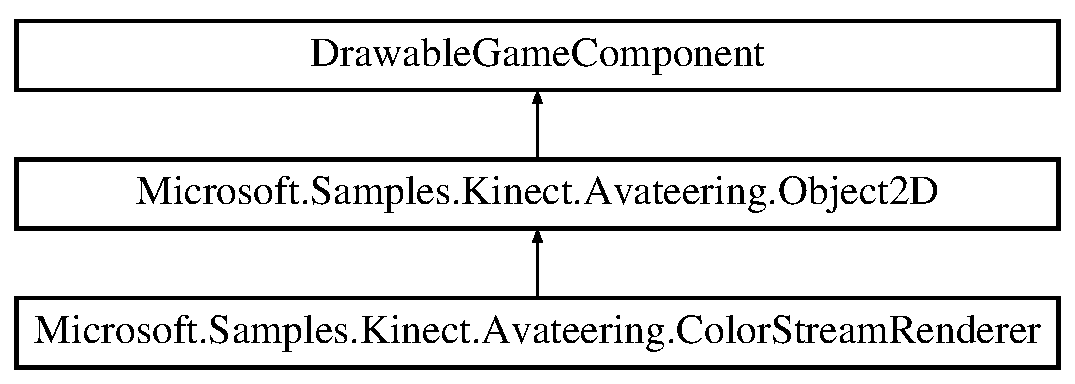
\includegraphics[height=3.000000cm]{class_microsoft_1_1_samples_1_1_kinect_1_1_avateering_1_1_color_stream_renderer}
\end{center}
\end{figure}
\subsection*{Public Member Functions}
\begin{DoxyCompactItemize}
\item 
\hyperlink{class_microsoft_1_1_samples_1_1_kinect_1_1_avateering_1_1_color_stream_renderer_af607dd1f65442db88e01a99018ec1735}{Color\+Stream\+Renderer} (Game game)
\begin{DoxyCompactList}\small\item\em Initializes a new instance of the \hyperlink{class_microsoft_1_1_samples_1_1_kinect_1_1_avateering_1_1_color_stream_renderer}{Color\+Stream\+Renderer} class. \end{DoxyCompactList}\item 
override void \hyperlink{class_microsoft_1_1_samples_1_1_kinect_1_1_avateering_1_1_color_stream_renderer_aa6e32fc3aae3a1f9b49d547dba63c033}{Initialize} ()
\begin{DoxyCompactList}\small\item\em Initializes the necessary children. \end{DoxyCompactList}\item 
override void \hyperlink{class_microsoft_1_1_samples_1_1_kinect_1_1_avateering_1_1_color_stream_renderer_a8d596f939054c20ac74cb349a1a6562c}{Update} (Game\+Time game\+Time)
\begin{DoxyCompactList}\small\item\em The update method where the new color frame is retrieved. \end{DoxyCompactList}\item 
override void \hyperlink{class_microsoft_1_1_samples_1_1_kinect_1_1_avateering_1_1_color_stream_renderer_aa0560415311dae0e40e0366abbe779a5}{Draw} (Game\+Time game\+Time)
\begin{DoxyCompactList}\small\item\em This method renders the color and skeleton frame. \end{DoxyCompactList}\end{DoxyCompactItemize}
\subsection*{Protected Member Functions}
\begin{DoxyCompactItemize}
\item 
override void \hyperlink{class_microsoft_1_1_samples_1_1_kinect_1_1_avateering_1_1_color_stream_renderer_af93996a406cb05d3ee779c94a2537d94}{Load\+Content} ()
\begin{DoxyCompactList}\small\item\em This method loads the Xna effect. \end{DoxyCompactList}\end{DoxyCompactItemize}
\subsection*{Additional Inherited Members}


\subsection{Detailed Description}
This class renders the current color stream frame. 



\subsection{Constructor \& Destructor Documentation}
\hypertarget{class_microsoft_1_1_samples_1_1_kinect_1_1_avateering_1_1_color_stream_renderer_af607dd1f65442db88e01a99018ec1735}{\index{Microsoft\+::\+Samples\+::\+Kinect\+::\+Avateering\+::\+Color\+Stream\+Renderer@{Microsoft\+::\+Samples\+::\+Kinect\+::\+Avateering\+::\+Color\+Stream\+Renderer}!Color\+Stream\+Renderer@{Color\+Stream\+Renderer}}
\index{Color\+Stream\+Renderer@{Color\+Stream\+Renderer}!Microsoft\+::\+Samples\+::\+Kinect\+::\+Avateering\+::\+Color\+Stream\+Renderer@{Microsoft\+::\+Samples\+::\+Kinect\+::\+Avateering\+::\+Color\+Stream\+Renderer}}
\subsubsection[{Color\+Stream\+Renderer}]{\setlength{\rightskip}{0pt plus 5cm}Microsoft.\+Samples.\+Kinect.\+Avateering.\+Color\+Stream\+Renderer.\+Color\+Stream\+Renderer (
\begin{DoxyParamCaption}
\item[{Game}]{game}
\end{DoxyParamCaption}
)}}\label{class_microsoft_1_1_samples_1_1_kinect_1_1_avateering_1_1_color_stream_renderer_af607dd1f65442db88e01a99018ec1735}


Initializes a new instance of the \hyperlink{class_microsoft_1_1_samples_1_1_kinect_1_1_avateering_1_1_color_stream_renderer}{Color\+Stream\+Renderer} class. 


\begin{DoxyParams}{Parameters}
{\em game} & The related game object.\\
\hline
\end{DoxyParams}


\subsection{Member Function Documentation}
\hypertarget{class_microsoft_1_1_samples_1_1_kinect_1_1_avateering_1_1_color_stream_renderer_aa0560415311dae0e40e0366abbe779a5}{\index{Microsoft\+::\+Samples\+::\+Kinect\+::\+Avateering\+::\+Color\+Stream\+Renderer@{Microsoft\+::\+Samples\+::\+Kinect\+::\+Avateering\+::\+Color\+Stream\+Renderer}!Draw@{Draw}}
\index{Draw@{Draw}!Microsoft\+::\+Samples\+::\+Kinect\+::\+Avateering\+::\+Color\+Stream\+Renderer@{Microsoft\+::\+Samples\+::\+Kinect\+::\+Avateering\+::\+Color\+Stream\+Renderer}}
\subsubsection[{Draw}]{\setlength{\rightskip}{0pt plus 5cm}override void Microsoft.\+Samples.\+Kinect.\+Avateering.\+Color\+Stream\+Renderer.\+Draw (
\begin{DoxyParamCaption}
\item[{Game\+Time}]{game\+Time}
\end{DoxyParamCaption}
)}}\label{class_microsoft_1_1_samples_1_1_kinect_1_1_avateering_1_1_color_stream_renderer_aa0560415311dae0e40e0366abbe779a5}


This method renders the color and skeleton frame. 


\begin{DoxyParams}{Parameters}
{\em game\+Time} & The elapsed game time.\\
\hline
\end{DoxyParams}
\hypertarget{class_microsoft_1_1_samples_1_1_kinect_1_1_avateering_1_1_color_stream_renderer_aa6e32fc3aae3a1f9b49d547dba63c033}{\index{Microsoft\+::\+Samples\+::\+Kinect\+::\+Avateering\+::\+Color\+Stream\+Renderer@{Microsoft\+::\+Samples\+::\+Kinect\+::\+Avateering\+::\+Color\+Stream\+Renderer}!Initialize@{Initialize}}
\index{Initialize@{Initialize}!Microsoft\+::\+Samples\+::\+Kinect\+::\+Avateering\+::\+Color\+Stream\+Renderer@{Microsoft\+::\+Samples\+::\+Kinect\+::\+Avateering\+::\+Color\+Stream\+Renderer}}
\subsubsection[{Initialize}]{\setlength{\rightskip}{0pt plus 5cm}override void Microsoft.\+Samples.\+Kinect.\+Avateering.\+Color\+Stream\+Renderer.\+Initialize (
\begin{DoxyParamCaption}
{}
\end{DoxyParamCaption}
)}}\label{class_microsoft_1_1_samples_1_1_kinect_1_1_avateering_1_1_color_stream_renderer_aa6e32fc3aae3a1f9b49d547dba63c033}


Initializes the necessary children. 

\hypertarget{class_microsoft_1_1_samples_1_1_kinect_1_1_avateering_1_1_color_stream_renderer_af93996a406cb05d3ee779c94a2537d94}{\index{Microsoft\+::\+Samples\+::\+Kinect\+::\+Avateering\+::\+Color\+Stream\+Renderer@{Microsoft\+::\+Samples\+::\+Kinect\+::\+Avateering\+::\+Color\+Stream\+Renderer}!Load\+Content@{Load\+Content}}
\index{Load\+Content@{Load\+Content}!Microsoft\+::\+Samples\+::\+Kinect\+::\+Avateering\+::\+Color\+Stream\+Renderer@{Microsoft\+::\+Samples\+::\+Kinect\+::\+Avateering\+::\+Color\+Stream\+Renderer}}
\subsubsection[{Load\+Content}]{\setlength{\rightskip}{0pt plus 5cm}override void Microsoft.\+Samples.\+Kinect.\+Avateering.\+Color\+Stream\+Renderer.\+Load\+Content (
\begin{DoxyParamCaption}
{}
\end{DoxyParamCaption}
)\hspace{0.3cm}{\ttfamily [protected]}}}\label{class_microsoft_1_1_samples_1_1_kinect_1_1_avateering_1_1_color_stream_renderer_af93996a406cb05d3ee779c94a2537d94}


This method loads the Xna effect. 

\hypertarget{class_microsoft_1_1_samples_1_1_kinect_1_1_avateering_1_1_color_stream_renderer_a8d596f939054c20ac74cb349a1a6562c}{\index{Microsoft\+::\+Samples\+::\+Kinect\+::\+Avateering\+::\+Color\+Stream\+Renderer@{Microsoft\+::\+Samples\+::\+Kinect\+::\+Avateering\+::\+Color\+Stream\+Renderer}!Update@{Update}}
\index{Update@{Update}!Microsoft\+::\+Samples\+::\+Kinect\+::\+Avateering\+::\+Color\+Stream\+Renderer@{Microsoft\+::\+Samples\+::\+Kinect\+::\+Avateering\+::\+Color\+Stream\+Renderer}}
\subsubsection[{Update}]{\setlength{\rightskip}{0pt plus 5cm}override void Microsoft.\+Samples.\+Kinect.\+Avateering.\+Color\+Stream\+Renderer.\+Update (
\begin{DoxyParamCaption}
\item[{Game\+Time}]{game\+Time}
\end{DoxyParamCaption}
)}}\label{class_microsoft_1_1_samples_1_1_kinect_1_1_avateering_1_1_color_stream_renderer_a8d596f939054c20ac74cb349a1a6562c}


The update method where the new color frame is retrieved. 


\begin{DoxyParams}{Parameters}
{\em game\+Time} & The elapsed game time.\\
\hline
\end{DoxyParams}


The documentation for this class was generated from the following file\+:\begin{DoxyCompactItemize}
\item 
Avateering/Color\+Stream\+Renderer.\+cs\end{DoxyCompactItemize}

\hypertarget{class_microsoft_1_1_samples_1_1_kinect_1_1_avateering_1_1_coordinate_cross}{\section{Microsoft.\+Samples.\+Kinect.\+Avateering.\+Coordinate\+Cross Class Reference}
\label{class_microsoft_1_1_samples_1_1_kinect_1_1_avateering_1_1_coordinate_cross}\index{Microsoft.\+Samples.\+Kinect.\+Avateering.\+Coordinate\+Cross@{Microsoft.\+Samples.\+Kinect.\+Avateering.\+Coordinate\+Cross}}
}


\hyperlink{class_microsoft_1_1_samples_1_1_kinect_1_1_avateering_1_1_coordinate_cross}{Coordinate\+Cross} Class -\/ draws a \hyperlink{class_microsoft_1_1_samples_1_1_kinect_1_1_avateering_1_1_coordinate_cross}{Coordinate\+Cross} in the current coordinate system X\+N\+A uses a right hand coordinate system +\+X (right) is Red +\+Y (up) is Green +\+Z (forward) is Blue  


Inheritance diagram for Microsoft.\+Samples.\+Kinect.\+Avateering.\+Coordinate\+Cross\+:\begin{figure}[H]
\begin{center}
\leavevmode
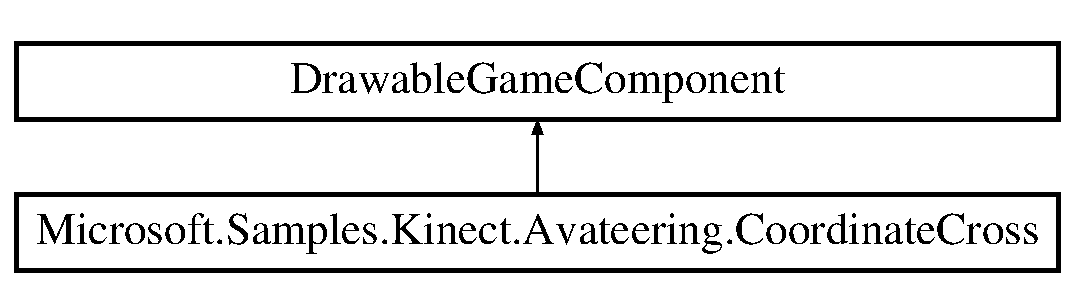
\includegraphics[height=2.000000cm]{class_microsoft_1_1_samples_1_1_kinect_1_1_avateering_1_1_coordinate_cross}
\end{center}
\end{figure}
\subsection*{Public Member Functions}
\begin{DoxyCompactItemize}
\item 
\hyperlink{class_microsoft_1_1_samples_1_1_kinect_1_1_avateering_1_1_coordinate_cross_a00b5eceee82d2b5bb39f8c7fcd3ea6c1}{Coordinate\+Cross} (Game game, float axis\+Length)
\begin{DoxyCompactList}\small\item\em Initializes a new instance of the \hyperlink{class_microsoft_1_1_samples_1_1_kinect_1_1_avateering_1_1_coordinate_cross}{Coordinate\+Cross} class. \end{DoxyCompactList}\item 
void \hyperlink{class_microsoft_1_1_samples_1_1_kinect_1_1_avateering_1_1_coordinate_cross_ada52632b099522d552c848487a448b4e}{Create\+Coordinate\+Cross} (float axis\+Length)
\begin{DoxyCompactList}\small\item\em Initializes a new instance of the Coordinate Cross class. \end{DoxyCompactList}\item 
void \hyperlink{class_microsoft_1_1_samples_1_1_kinect_1_1_avateering_1_1_coordinate_cross_acb449d7ad4361a931588dd7568c30457}{Draw} (Game\+Time game\+Time, Matrix world, Matrix view, Matrix projection)
\begin{DoxyCompactList}\small\item\em This method renders the current state. \end{DoxyCompactList}\end{DoxyCompactItemize}
\subsection*{Protected Member Functions}
\begin{DoxyCompactItemize}
\item 
override void \hyperlink{class_microsoft_1_1_samples_1_1_kinect_1_1_avateering_1_1_coordinate_cross_a5191669216fb474d855e29bd8e9bb187}{Load\+Content} ()
\begin{DoxyCompactList}\small\item\em This method loads the basic effect used for drawing. \end{DoxyCompactList}\end{DoxyCompactItemize}


\subsection{Detailed Description}
\hyperlink{class_microsoft_1_1_samples_1_1_kinect_1_1_avateering_1_1_coordinate_cross}{Coordinate\+Cross} Class -\/ draws a \hyperlink{class_microsoft_1_1_samples_1_1_kinect_1_1_avateering_1_1_coordinate_cross}{Coordinate\+Cross} in the current coordinate system X\+N\+A uses a right hand coordinate system +\+X (right) is Red +\+Y (up) is Green +\+Z (forward) is Blue 



\subsection{Constructor \& Destructor Documentation}
\hypertarget{class_microsoft_1_1_samples_1_1_kinect_1_1_avateering_1_1_coordinate_cross_a00b5eceee82d2b5bb39f8c7fcd3ea6c1}{\index{Microsoft\+::\+Samples\+::\+Kinect\+::\+Avateering\+::\+Coordinate\+Cross@{Microsoft\+::\+Samples\+::\+Kinect\+::\+Avateering\+::\+Coordinate\+Cross}!Coordinate\+Cross@{Coordinate\+Cross}}
\index{Coordinate\+Cross@{Coordinate\+Cross}!Microsoft\+::\+Samples\+::\+Kinect\+::\+Avateering\+::\+Coordinate\+Cross@{Microsoft\+::\+Samples\+::\+Kinect\+::\+Avateering\+::\+Coordinate\+Cross}}
\subsubsection[{Coordinate\+Cross}]{\setlength{\rightskip}{0pt plus 5cm}Microsoft.\+Samples.\+Kinect.\+Avateering.\+Coordinate\+Cross.\+Coordinate\+Cross (
\begin{DoxyParamCaption}
\item[{Game}]{game, }
\item[{float}]{axis\+Length}
\end{DoxyParamCaption}
)}}\label{class_microsoft_1_1_samples_1_1_kinect_1_1_avateering_1_1_coordinate_cross_a00b5eceee82d2b5bb39f8c7fcd3ea6c1}


Initializes a new instance of the \hyperlink{class_microsoft_1_1_samples_1_1_kinect_1_1_avateering_1_1_coordinate_cross}{Coordinate\+Cross} class. 


\begin{DoxyParams}{Parameters}
{\em game} & The related game object.\\
\hline
{\em axis\+Length} & The length of the axis in 3\+D units.\\
\hline
\end{DoxyParams}


\subsection{Member Function Documentation}
\hypertarget{class_microsoft_1_1_samples_1_1_kinect_1_1_avateering_1_1_coordinate_cross_ada52632b099522d552c848487a448b4e}{\index{Microsoft\+::\+Samples\+::\+Kinect\+::\+Avateering\+::\+Coordinate\+Cross@{Microsoft\+::\+Samples\+::\+Kinect\+::\+Avateering\+::\+Coordinate\+Cross}!Create\+Coordinate\+Cross@{Create\+Coordinate\+Cross}}
\index{Create\+Coordinate\+Cross@{Create\+Coordinate\+Cross}!Microsoft\+::\+Samples\+::\+Kinect\+::\+Avateering\+::\+Coordinate\+Cross@{Microsoft\+::\+Samples\+::\+Kinect\+::\+Avateering\+::\+Coordinate\+Cross}}
\subsubsection[{Create\+Coordinate\+Cross}]{\setlength{\rightskip}{0pt plus 5cm}void Microsoft.\+Samples.\+Kinect.\+Avateering.\+Coordinate\+Cross.\+Create\+Coordinate\+Cross (
\begin{DoxyParamCaption}
\item[{float}]{axis\+Length}
\end{DoxyParamCaption}
)}}\label{class_microsoft_1_1_samples_1_1_kinect_1_1_avateering_1_1_coordinate_cross_ada52632b099522d552c848487a448b4e}


Initializes a new instance of the Coordinate Cross class. 


\begin{DoxyParams}{Parameters}
{\em axis\+Length} & The length of the axis in 3\+D units.\\
\hline
\end{DoxyParams}
\hypertarget{class_microsoft_1_1_samples_1_1_kinect_1_1_avateering_1_1_coordinate_cross_acb449d7ad4361a931588dd7568c30457}{\index{Microsoft\+::\+Samples\+::\+Kinect\+::\+Avateering\+::\+Coordinate\+Cross@{Microsoft\+::\+Samples\+::\+Kinect\+::\+Avateering\+::\+Coordinate\+Cross}!Draw@{Draw}}
\index{Draw@{Draw}!Microsoft\+::\+Samples\+::\+Kinect\+::\+Avateering\+::\+Coordinate\+Cross@{Microsoft\+::\+Samples\+::\+Kinect\+::\+Avateering\+::\+Coordinate\+Cross}}
\subsubsection[{Draw}]{\setlength{\rightskip}{0pt plus 5cm}void Microsoft.\+Samples.\+Kinect.\+Avateering.\+Coordinate\+Cross.\+Draw (
\begin{DoxyParamCaption}
\item[{Game\+Time}]{game\+Time, }
\item[{Matrix}]{world, }
\item[{Matrix}]{view, }
\item[{Matrix}]{projection}
\end{DoxyParamCaption}
)}}\label{class_microsoft_1_1_samples_1_1_kinect_1_1_avateering_1_1_coordinate_cross_acb449d7ad4361a931588dd7568c30457}


This method renders the current state. 


\begin{DoxyParams}{Parameters}
{\em game\+Time} & The elapsed game time.\\
\hline
{\em world} & The world matrix.\\
\hline
{\em view} & The view matrix.\\
\hline
{\em projection} & The projection matrix.\\
\hline
\end{DoxyParams}
\hypertarget{class_microsoft_1_1_samples_1_1_kinect_1_1_avateering_1_1_coordinate_cross_a5191669216fb474d855e29bd8e9bb187}{\index{Microsoft\+::\+Samples\+::\+Kinect\+::\+Avateering\+::\+Coordinate\+Cross@{Microsoft\+::\+Samples\+::\+Kinect\+::\+Avateering\+::\+Coordinate\+Cross}!Load\+Content@{Load\+Content}}
\index{Load\+Content@{Load\+Content}!Microsoft\+::\+Samples\+::\+Kinect\+::\+Avateering\+::\+Coordinate\+Cross@{Microsoft\+::\+Samples\+::\+Kinect\+::\+Avateering\+::\+Coordinate\+Cross}}
\subsubsection[{Load\+Content}]{\setlength{\rightskip}{0pt plus 5cm}override void Microsoft.\+Samples.\+Kinect.\+Avateering.\+Coordinate\+Cross.\+Load\+Content (
\begin{DoxyParamCaption}
{}
\end{DoxyParamCaption}
)\hspace{0.3cm}{\ttfamily [protected]}}}\label{class_microsoft_1_1_samples_1_1_kinect_1_1_avateering_1_1_coordinate_cross_a5191669216fb474d855e29bd8e9bb187}


This method loads the basic effect used for drawing. 



The documentation for this class was generated from the following file\+:\begin{DoxyCompactItemize}
\item 
Avateering/Coordinate\+Cross.\+cs\end{DoxyCompactItemize}

\hypertarget{class_microsoft_1_1_samples_1_1_kinect_1_1_avateering_1_1_depth_stream_renderer}{\section{Microsoft.\+Samples.\+Kinect.\+Avateering.\+Depth\+Stream\+Renderer Class Reference}
\label{class_microsoft_1_1_samples_1_1_kinect_1_1_avateering_1_1_depth_stream_renderer}\index{Microsoft.\+Samples.\+Kinect.\+Avateering.\+Depth\+Stream\+Renderer@{Microsoft.\+Samples.\+Kinect.\+Avateering.\+Depth\+Stream\+Renderer}}
}


This class renders the current depth stream frame.  


Inheritance diagram for Microsoft.\+Samples.\+Kinect.\+Avateering.\+Depth\+Stream\+Renderer\+:\begin{figure}[H]
\begin{center}
\leavevmode
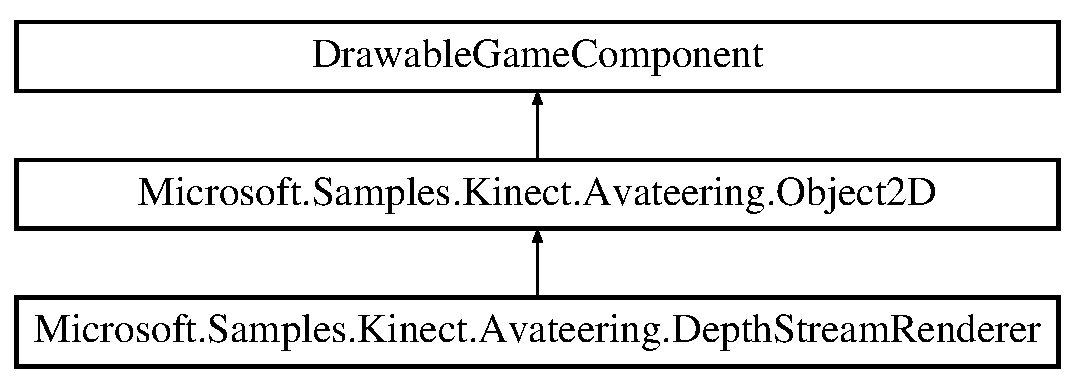
\includegraphics[height=3.000000cm]{class_microsoft_1_1_samples_1_1_kinect_1_1_avateering_1_1_depth_stream_renderer}
\end{center}
\end{figure}
\subsection*{Public Member Functions}
\begin{DoxyCompactItemize}
\item 
\hyperlink{class_microsoft_1_1_samples_1_1_kinect_1_1_avateering_1_1_depth_stream_renderer_a7c2b33729bd434ec17bf5488c8977429}{Depth\+Stream\+Renderer} (Game game)
\begin{DoxyCompactList}\small\item\em Initializes a new instance of the \hyperlink{class_microsoft_1_1_samples_1_1_kinect_1_1_avateering_1_1_depth_stream_renderer}{Depth\+Stream\+Renderer} class. \end{DoxyCompactList}\item 
override void \hyperlink{class_microsoft_1_1_samples_1_1_kinect_1_1_avateering_1_1_depth_stream_renderer_ad45239b592f01487e492740a43e63ba2}{Initialize} ()
\begin{DoxyCompactList}\small\item\em Initializes the necessary children. \end{DoxyCompactList}\item 
override void \hyperlink{class_microsoft_1_1_samples_1_1_kinect_1_1_avateering_1_1_depth_stream_renderer_a365af6c9d57d70df4921d6f7ea2ba90e}{Update} (Game\+Time game\+Time)
\begin{DoxyCompactList}\small\item\em The update method where the new depth frame is retrieved. \end{DoxyCompactList}\item 
override void \hyperlink{class_microsoft_1_1_samples_1_1_kinect_1_1_avateering_1_1_depth_stream_renderer_a975a1d4c53be24b3336110fa2985a68f}{Draw} (Game\+Time game\+Time)
\begin{DoxyCompactList}\small\item\em This method renders the color and skeleton frame. \end{DoxyCompactList}\end{DoxyCompactItemize}
\subsection*{Protected Member Functions}
\begin{DoxyCompactItemize}
\item 
override void \hyperlink{class_microsoft_1_1_samples_1_1_kinect_1_1_avateering_1_1_depth_stream_renderer_a2781c13877e0081c4d4e2ba49766909b}{Load\+Content} ()
\begin{DoxyCompactList}\small\item\em This method loads the Xna effect. \end{DoxyCompactList}\end{DoxyCompactItemize}
\subsection*{Properties}
\begin{DoxyCompactItemize}
\item 
Sprite\+Batch \hyperlink{class_microsoft_1_1_samples_1_1_kinect_1_1_avateering_1_1_depth_stream_renderer_aceaaf8ce615e328934f79619de246878}{Shared\+Sprite\+Batch}\hspace{0.3cm}{\ttfamily  \mbox{[}get\mbox{]}}
\begin{DoxyCompactList}\small\item\em Gets the Sprite\+Batch from the services. \end{DoxyCompactList}\end{DoxyCompactItemize}


\subsection{Detailed Description}
This class renders the current depth stream frame. 



\subsection{Constructor \& Destructor Documentation}
\hypertarget{class_microsoft_1_1_samples_1_1_kinect_1_1_avateering_1_1_depth_stream_renderer_a7c2b33729bd434ec17bf5488c8977429}{\index{Microsoft\+::\+Samples\+::\+Kinect\+::\+Avateering\+::\+Depth\+Stream\+Renderer@{Microsoft\+::\+Samples\+::\+Kinect\+::\+Avateering\+::\+Depth\+Stream\+Renderer}!Depth\+Stream\+Renderer@{Depth\+Stream\+Renderer}}
\index{Depth\+Stream\+Renderer@{Depth\+Stream\+Renderer}!Microsoft\+::\+Samples\+::\+Kinect\+::\+Avateering\+::\+Depth\+Stream\+Renderer@{Microsoft\+::\+Samples\+::\+Kinect\+::\+Avateering\+::\+Depth\+Stream\+Renderer}}
\subsubsection[{Depth\+Stream\+Renderer}]{\setlength{\rightskip}{0pt plus 5cm}Microsoft.\+Samples.\+Kinect.\+Avateering.\+Depth\+Stream\+Renderer.\+Depth\+Stream\+Renderer (
\begin{DoxyParamCaption}
\item[{Game}]{game}
\end{DoxyParamCaption}
)}}\label{class_microsoft_1_1_samples_1_1_kinect_1_1_avateering_1_1_depth_stream_renderer_a7c2b33729bd434ec17bf5488c8977429}


Initializes a new instance of the \hyperlink{class_microsoft_1_1_samples_1_1_kinect_1_1_avateering_1_1_depth_stream_renderer}{Depth\+Stream\+Renderer} class. 


\begin{DoxyParams}{Parameters}
{\em game} & The related game object.\\
\hline
\end{DoxyParams}


\subsection{Member Function Documentation}
\hypertarget{class_microsoft_1_1_samples_1_1_kinect_1_1_avateering_1_1_depth_stream_renderer_a975a1d4c53be24b3336110fa2985a68f}{\index{Microsoft\+::\+Samples\+::\+Kinect\+::\+Avateering\+::\+Depth\+Stream\+Renderer@{Microsoft\+::\+Samples\+::\+Kinect\+::\+Avateering\+::\+Depth\+Stream\+Renderer}!Draw@{Draw}}
\index{Draw@{Draw}!Microsoft\+::\+Samples\+::\+Kinect\+::\+Avateering\+::\+Depth\+Stream\+Renderer@{Microsoft\+::\+Samples\+::\+Kinect\+::\+Avateering\+::\+Depth\+Stream\+Renderer}}
\subsubsection[{Draw}]{\setlength{\rightskip}{0pt plus 5cm}override void Microsoft.\+Samples.\+Kinect.\+Avateering.\+Depth\+Stream\+Renderer.\+Draw (
\begin{DoxyParamCaption}
\item[{Game\+Time}]{game\+Time}
\end{DoxyParamCaption}
)}}\label{class_microsoft_1_1_samples_1_1_kinect_1_1_avateering_1_1_depth_stream_renderer_a975a1d4c53be24b3336110fa2985a68f}


This method renders the color and skeleton frame. 


\begin{DoxyParams}{Parameters}
{\em game\+Time} & The elapsed game time.\\
\hline
\end{DoxyParams}
\hypertarget{class_microsoft_1_1_samples_1_1_kinect_1_1_avateering_1_1_depth_stream_renderer_ad45239b592f01487e492740a43e63ba2}{\index{Microsoft\+::\+Samples\+::\+Kinect\+::\+Avateering\+::\+Depth\+Stream\+Renderer@{Microsoft\+::\+Samples\+::\+Kinect\+::\+Avateering\+::\+Depth\+Stream\+Renderer}!Initialize@{Initialize}}
\index{Initialize@{Initialize}!Microsoft\+::\+Samples\+::\+Kinect\+::\+Avateering\+::\+Depth\+Stream\+Renderer@{Microsoft\+::\+Samples\+::\+Kinect\+::\+Avateering\+::\+Depth\+Stream\+Renderer}}
\subsubsection[{Initialize}]{\setlength{\rightskip}{0pt plus 5cm}override void Microsoft.\+Samples.\+Kinect.\+Avateering.\+Depth\+Stream\+Renderer.\+Initialize (
\begin{DoxyParamCaption}
{}
\end{DoxyParamCaption}
)}}\label{class_microsoft_1_1_samples_1_1_kinect_1_1_avateering_1_1_depth_stream_renderer_ad45239b592f01487e492740a43e63ba2}


Initializes the necessary children. 

\hypertarget{class_microsoft_1_1_samples_1_1_kinect_1_1_avateering_1_1_depth_stream_renderer_a2781c13877e0081c4d4e2ba49766909b}{\index{Microsoft\+::\+Samples\+::\+Kinect\+::\+Avateering\+::\+Depth\+Stream\+Renderer@{Microsoft\+::\+Samples\+::\+Kinect\+::\+Avateering\+::\+Depth\+Stream\+Renderer}!Load\+Content@{Load\+Content}}
\index{Load\+Content@{Load\+Content}!Microsoft\+::\+Samples\+::\+Kinect\+::\+Avateering\+::\+Depth\+Stream\+Renderer@{Microsoft\+::\+Samples\+::\+Kinect\+::\+Avateering\+::\+Depth\+Stream\+Renderer}}
\subsubsection[{Load\+Content}]{\setlength{\rightskip}{0pt plus 5cm}override void Microsoft.\+Samples.\+Kinect.\+Avateering.\+Depth\+Stream\+Renderer.\+Load\+Content (
\begin{DoxyParamCaption}
{}
\end{DoxyParamCaption}
)\hspace{0.3cm}{\ttfamily [protected]}}}\label{class_microsoft_1_1_samples_1_1_kinect_1_1_avateering_1_1_depth_stream_renderer_a2781c13877e0081c4d4e2ba49766909b}


This method loads the Xna effect. 

\hypertarget{class_microsoft_1_1_samples_1_1_kinect_1_1_avateering_1_1_depth_stream_renderer_a365af6c9d57d70df4921d6f7ea2ba90e}{\index{Microsoft\+::\+Samples\+::\+Kinect\+::\+Avateering\+::\+Depth\+Stream\+Renderer@{Microsoft\+::\+Samples\+::\+Kinect\+::\+Avateering\+::\+Depth\+Stream\+Renderer}!Update@{Update}}
\index{Update@{Update}!Microsoft\+::\+Samples\+::\+Kinect\+::\+Avateering\+::\+Depth\+Stream\+Renderer@{Microsoft\+::\+Samples\+::\+Kinect\+::\+Avateering\+::\+Depth\+Stream\+Renderer}}
\subsubsection[{Update}]{\setlength{\rightskip}{0pt plus 5cm}override void Microsoft.\+Samples.\+Kinect.\+Avateering.\+Depth\+Stream\+Renderer.\+Update (
\begin{DoxyParamCaption}
\item[{Game\+Time}]{game\+Time}
\end{DoxyParamCaption}
)}}\label{class_microsoft_1_1_samples_1_1_kinect_1_1_avateering_1_1_depth_stream_renderer_a365af6c9d57d70df4921d6f7ea2ba90e}


The update method where the new depth frame is retrieved. 


\begin{DoxyParams}{Parameters}
{\em game\+Time} & The elapsed game time.\\
\hline
\end{DoxyParams}


\subsection{Property Documentation}
\hypertarget{class_microsoft_1_1_samples_1_1_kinect_1_1_avateering_1_1_depth_stream_renderer_aceaaf8ce615e328934f79619de246878}{\index{Microsoft\+::\+Samples\+::\+Kinect\+::\+Avateering\+::\+Depth\+Stream\+Renderer@{Microsoft\+::\+Samples\+::\+Kinect\+::\+Avateering\+::\+Depth\+Stream\+Renderer}!Shared\+Sprite\+Batch@{Shared\+Sprite\+Batch}}
\index{Shared\+Sprite\+Batch@{Shared\+Sprite\+Batch}!Microsoft\+::\+Samples\+::\+Kinect\+::\+Avateering\+::\+Depth\+Stream\+Renderer@{Microsoft\+::\+Samples\+::\+Kinect\+::\+Avateering\+::\+Depth\+Stream\+Renderer}}
\subsubsection[{Shared\+Sprite\+Batch}]{\setlength{\rightskip}{0pt plus 5cm}Sprite\+Batch Microsoft.\+Samples.\+Kinect.\+Avateering.\+Depth\+Stream\+Renderer.\+Shared\+Sprite\+Batch\hspace{0.3cm}{\ttfamily [get]}}}\label{class_microsoft_1_1_samples_1_1_kinect_1_1_avateering_1_1_depth_stream_renderer_aceaaf8ce615e328934f79619de246878}


Gets the Sprite\+Batch from the services. 



The documentation for this class was generated from the following file\+:\begin{DoxyCompactItemize}
\item 
Avateering/Depth\+Stream\+Renderer.\+cs\end{DoxyCompactItemize}

\hypertarget{class_microsoft_1_1_samples_1_1_kinect_1_1_avateering_1_1_grid_xz}{\section{Microsoft.\+Samples.\+Kinect.\+Avateering.\+Grid\+Xz Class Reference}
\label{class_microsoft_1_1_samples_1_1_kinect_1_1_avateering_1_1_grid_xz}\index{Microsoft.\+Samples.\+Kinect.\+Avateering.\+Grid\+Xz@{Microsoft.\+Samples.\+Kinect.\+Avateering.\+Grid\+Xz}}
}


Grid\+X\+Z Class -\/ draws a grid in X\+Z plane  


Inheritance diagram for Microsoft.\+Samples.\+Kinect.\+Avateering.\+Grid\+Xz\+:\begin{figure}[H]
\begin{center}
\leavevmode
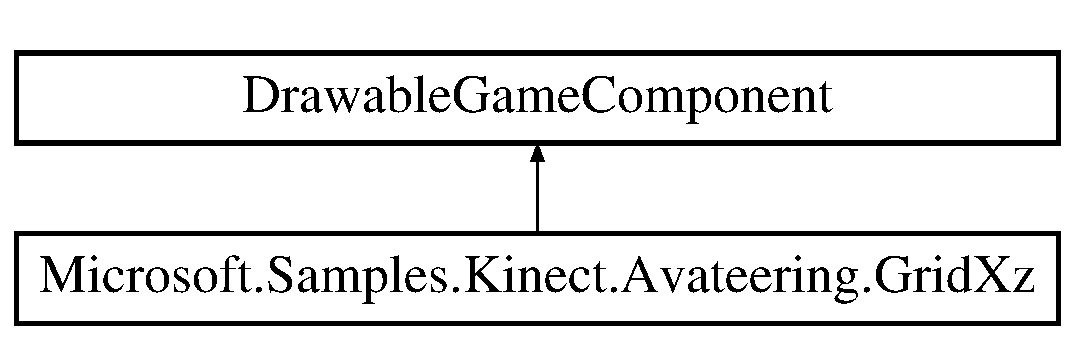
\includegraphics[height=2.000000cm]{class_microsoft_1_1_samples_1_1_kinect_1_1_avateering_1_1_grid_xz}
\end{center}
\end{figure}
\subsection*{Public Member Functions}
\begin{DoxyCompactItemize}
\item 
\hyperlink{class_microsoft_1_1_samples_1_1_kinect_1_1_avateering_1_1_grid_xz_ac09b225053a47086ce0b346959f7daf9}{Grid\+Xz} (Game game, Vector3 origin, Vector2 grid\+Size, Vector2 number\+Of\+Rows\+And\+Columns, Color grid\+Color)
\begin{DoxyCompactList}\small\item\em Initializes a new instance of the \hyperlink{class_microsoft_1_1_samples_1_1_kinect_1_1_avateering_1_1_grid_xz}{Grid\+Xz} class. \end{DoxyCompactList}\item 
void \hyperlink{class_microsoft_1_1_samples_1_1_kinect_1_1_avateering_1_1_grid_xz_a19e9796b69d18b7c244d027c99e3828c}{Create\+Grid} (Vector3 origin, Vector2 grid\+Size, Vector2 number\+Of\+Rows\+And\+Columns, Color grid\+Color)
\begin{DoxyCompactList}\small\item\em Create the Grid. \end{DoxyCompactList}\item 
void \hyperlink{class_microsoft_1_1_samples_1_1_kinect_1_1_avateering_1_1_grid_xz_add707450b8720901a9470c71d0848fee}{Draw} (Game\+Time game\+Time, Matrix world, Matrix view, Matrix projection)
\begin{DoxyCompactList}\small\item\em This method renders the current state. \end{DoxyCompactList}\end{DoxyCompactItemize}
\subsection*{Protected Member Functions}
\begin{DoxyCompactItemize}
\item 
override void \hyperlink{class_microsoft_1_1_samples_1_1_kinect_1_1_avateering_1_1_grid_xz_ab6b87bcfffced83a73299d0cd740520c}{Load\+Content} ()
\begin{DoxyCompactList}\small\item\em This method loads the basic effect used for drawing. \end{DoxyCompactList}\end{DoxyCompactItemize}


\subsection{Detailed Description}
Grid\+X\+Z Class -\/ draws a grid in X\+Z plane 



\subsection{Constructor \& Destructor Documentation}
\hypertarget{class_microsoft_1_1_samples_1_1_kinect_1_1_avateering_1_1_grid_xz_ac09b225053a47086ce0b346959f7daf9}{\index{Microsoft\+::\+Samples\+::\+Kinect\+::\+Avateering\+::\+Grid\+Xz@{Microsoft\+::\+Samples\+::\+Kinect\+::\+Avateering\+::\+Grid\+Xz}!Grid\+Xz@{Grid\+Xz}}
\index{Grid\+Xz@{Grid\+Xz}!Microsoft\+::\+Samples\+::\+Kinect\+::\+Avateering\+::\+Grid\+Xz@{Microsoft\+::\+Samples\+::\+Kinect\+::\+Avateering\+::\+Grid\+Xz}}
\subsubsection[{Grid\+Xz}]{\setlength{\rightskip}{0pt plus 5cm}Microsoft.\+Samples.\+Kinect.\+Avateering.\+Grid\+Xz.\+Grid\+Xz (
\begin{DoxyParamCaption}
\item[{Game}]{game, }
\item[{Vector3}]{origin, }
\item[{Vector2}]{grid\+Size, }
\item[{Vector2}]{number\+Of\+Rows\+And\+Columns, }
\item[{Color}]{grid\+Color}
\end{DoxyParamCaption}
)}}\label{class_microsoft_1_1_samples_1_1_kinect_1_1_avateering_1_1_grid_xz_ac09b225053a47086ce0b346959f7daf9}


Initializes a new instance of the \hyperlink{class_microsoft_1_1_samples_1_1_kinect_1_1_avateering_1_1_grid_xz}{Grid\+Xz} class. 


\begin{DoxyParams}{Parameters}
{\em game} & The related game object.\\
\hline
{\em origin} & The origin of the grid is 3\+D world coordinates.\\
\hline
{\em grid\+Size} & The size of the grid.\\
\hline
{\em number\+Of\+Rows\+And\+Columns} & The number of rows in the grid in X and number of columns in Y.\\
\hline
{\em grid\+Color} & The color of the grid lines.\\
\hline
\end{DoxyParams}


\subsection{Member Function Documentation}
\hypertarget{class_microsoft_1_1_samples_1_1_kinect_1_1_avateering_1_1_grid_xz_a19e9796b69d18b7c244d027c99e3828c}{\index{Microsoft\+::\+Samples\+::\+Kinect\+::\+Avateering\+::\+Grid\+Xz@{Microsoft\+::\+Samples\+::\+Kinect\+::\+Avateering\+::\+Grid\+Xz}!Create\+Grid@{Create\+Grid}}
\index{Create\+Grid@{Create\+Grid}!Microsoft\+::\+Samples\+::\+Kinect\+::\+Avateering\+::\+Grid\+Xz@{Microsoft\+::\+Samples\+::\+Kinect\+::\+Avateering\+::\+Grid\+Xz}}
\subsubsection[{Create\+Grid}]{\setlength{\rightskip}{0pt plus 5cm}void Microsoft.\+Samples.\+Kinect.\+Avateering.\+Grid\+Xz.\+Create\+Grid (
\begin{DoxyParamCaption}
\item[{Vector3}]{origin, }
\item[{Vector2}]{grid\+Size, }
\item[{Vector2}]{number\+Of\+Rows\+And\+Columns, }
\item[{Color}]{grid\+Color}
\end{DoxyParamCaption}
)}}\label{class_microsoft_1_1_samples_1_1_kinect_1_1_avateering_1_1_grid_xz_a19e9796b69d18b7c244d027c99e3828c}


Create the Grid. 


\begin{DoxyParams}{Parameters}
{\em origin} & The origin of the grid is 3\+D world coordinates.\\
\hline
{\em grid\+Size} & The size of the grid.\\
\hline
{\em number\+Of\+Rows\+And\+Columns} & The number of rows in the grid in X and number of columns in Y.\\
\hline
{\em grid\+Color} & The color of the grid lines.\\
\hline
\end{DoxyParams}
\hypertarget{class_microsoft_1_1_samples_1_1_kinect_1_1_avateering_1_1_grid_xz_add707450b8720901a9470c71d0848fee}{\index{Microsoft\+::\+Samples\+::\+Kinect\+::\+Avateering\+::\+Grid\+Xz@{Microsoft\+::\+Samples\+::\+Kinect\+::\+Avateering\+::\+Grid\+Xz}!Draw@{Draw}}
\index{Draw@{Draw}!Microsoft\+::\+Samples\+::\+Kinect\+::\+Avateering\+::\+Grid\+Xz@{Microsoft\+::\+Samples\+::\+Kinect\+::\+Avateering\+::\+Grid\+Xz}}
\subsubsection[{Draw}]{\setlength{\rightskip}{0pt plus 5cm}void Microsoft.\+Samples.\+Kinect.\+Avateering.\+Grid\+Xz.\+Draw (
\begin{DoxyParamCaption}
\item[{Game\+Time}]{game\+Time, }
\item[{Matrix}]{world, }
\item[{Matrix}]{view, }
\item[{Matrix}]{projection}
\end{DoxyParamCaption}
)}}\label{class_microsoft_1_1_samples_1_1_kinect_1_1_avateering_1_1_grid_xz_add707450b8720901a9470c71d0848fee}


This method renders the current state. 


\begin{DoxyParams}{Parameters}
{\em game\+Time} & The elapsed game time.\\
\hline
{\em world} & The world matrix.\\
\hline
{\em view} & The view matrix.\\
\hline
{\em projection} & The projection matrix.\\
\hline
\end{DoxyParams}
\hypertarget{class_microsoft_1_1_samples_1_1_kinect_1_1_avateering_1_1_grid_xz_ab6b87bcfffced83a73299d0cd740520c}{\index{Microsoft\+::\+Samples\+::\+Kinect\+::\+Avateering\+::\+Grid\+Xz@{Microsoft\+::\+Samples\+::\+Kinect\+::\+Avateering\+::\+Grid\+Xz}!Load\+Content@{Load\+Content}}
\index{Load\+Content@{Load\+Content}!Microsoft\+::\+Samples\+::\+Kinect\+::\+Avateering\+::\+Grid\+Xz@{Microsoft\+::\+Samples\+::\+Kinect\+::\+Avateering\+::\+Grid\+Xz}}
\subsubsection[{Load\+Content}]{\setlength{\rightskip}{0pt plus 5cm}override void Microsoft.\+Samples.\+Kinect.\+Avateering.\+Grid\+Xz.\+Load\+Content (
\begin{DoxyParamCaption}
{}
\end{DoxyParamCaption}
)\hspace{0.3cm}{\ttfamily [protected]}}}\label{class_microsoft_1_1_samples_1_1_kinect_1_1_avateering_1_1_grid_xz_ab6b87bcfffced83a73299d0cd740520c}


This method loads the basic effect used for drawing. 



The documentation for this class was generated from the following file\+:\begin{DoxyCompactItemize}
\item 
Avateering/Grid\+X\+Z.\+cs\end{DoxyCompactItemize}

\hypertarget{class_microsoft_1_1_samples_1_1_kinect_1_1_avateering_1_1_kinect_chooser}{\section{Microsoft.\+Samples.\+Kinect.\+Avateering.\+Kinect\+Chooser Class Reference}
\label{class_microsoft_1_1_samples_1_1_kinect_1_1_avateering_1_1_kinect_chooser}\index{Microsoft.\+Samples.\+Kinect.\+Avateering.\+Kinect\+Chooser@{Microsoft.\+Samples.\+Kinect.\+Avateering.\+Kinect\+Chooser}}
}


This class will pick a \hyperlink{namespace_microsoft_1_1_samples_1_1_kinect}{Kinect} sensor, if available.  


Inheritance diagram for Microsoft.\+Samples.\+Kinect.\+Avateering.\+Kinect\+Chooser\+:\begin{figure}[H]
\begin{center}
\leavevmode
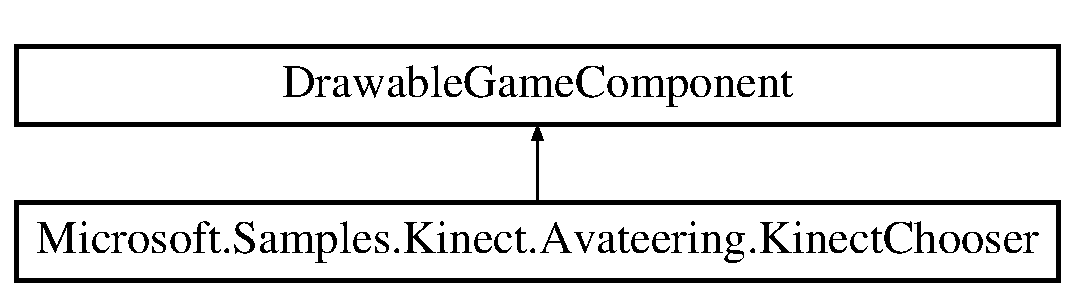
\includegraphics[height=2.000000cm]{class_microsoft_1_1_samples_1_1_kinect_1_1_avateering_1_1_kinect_chooser}
\end{center}
\end{figure}
\subsection*{Public Member Functions}
\begin{DoxyCompactItemize}
\item 
\hyperlink{class_microsoft_1_1_samples_1_1_kinect_1_1_avateering_1_1_kinect_chooser_a29881c15d2fce5627afaf44aedebb167}{Kinect\+Chooser} (Game game, Color\+Image\+Format color\+Format, Depth\+Image\+Format depth\+Format)
\begin{DoxyCompactList}\small\item\em Initializes a new instance of the \hyperlink{class_microsoft_1_1_samples_1_1_kinect_1_1_avateering_1_1_kinect_chooser}{Kinect\+Chooser} class. \end{DoxyCompactList}\item 
override void \hyperlink{class_microsoft_1_1_samples_1_1_kinect_1_1_avateering_1_1_kinect_chooser_a2a64601325b25988ed098dffbe304b85}{Draw} (Game\+Time game\+Time)
\begin{DoxyCompactList}\small\item\em This method renders the current state of the \hyperlink{class_microsoft_1_1_samples_1_1_kinect_1_1_avateering_1_1_kinect_chooser}{Kinect\+Chooser}. \end{DoxyCompactList}\end{DoxyCompactItemize}
\subsection*{Protected Member Functions}
\begin{DoxyCompactItemize}
\item 
override void \hyperlink{class_microsoft_1_1_samples_1_1_kinect_1_1_avateering_1_1_kinect_chooser_a4522920e8cdfb10fef30d242fcb92523}{Load\+Content} ()
\begin{DoxyCompactList}\small\item\em This method loads the textures and fonts. \end{DoxyCompactList}\item 
override void \hyperlink{class_microsoft_1_1_samples_1_1_kinect_1_1_avateering_1_1_kinect_chooser_a7ef341c7a8390e715f93c2a73ecb1e86}{Unload\+Content} ()
\begin{DoxyCompactList}\small\item\em This method ensures that the Kinect\+Sensor is stopped before exiting. \end{DoxyCompactList}\end{DoxyCompactItemize}
\subsection*{Properties}
\begin{DoxyCompactItemize}
\item 
Sprite\+Batch \hyperlink{class_microsoft_1_1_samples_1_1_kinect_1_1_avateering_1_1_kinect_chooser_a0a11686b3a34bd60af0322f281743c49}{Shared\+Sprite\+Batch}\hspace{0.3cm}{\ttfamily  \mbox{[}get\mbox{]}}
\begin{DoxyCompactList}\small\item\em Gets the Sprite\+Batch from the services. \end{DoxyCompactList}\item 
Kinect\+Sensor \hyperlink{class_microsoft_1_1_samples_1_1_kinect_1_1_avateering_1_1_kinect_chooser_a6b75400ac959ae1dca6df7361c9d70c7}{Sensor}\hspace{0.3cm}{\ttfamily  \mbox{[}get, set\mbox{]}}
\begin{DoxyCompactList}\small\item\em Gets the selected Kinect\+Sensor. \end{DoxyCompactList}\item 
Kinect\+Status \hyperlink{class_microsoft_1_1_samples_1_1_kinect_1_1_avateering_1_1_kinect_chooser_aca4cdae78c86075fc6231d089874eb19}{Last\+Status}\hspace{0.3cm}{\ttfamily  \mbox{[}get, set\mbox{]}}
\begin{DoxyCompactList}\small\item\em Gets the last known status of the Kinect\+Sensor. \end{DoxyCompactList}\item 
bool \hyperlink{class_microsoft_1_1_samples_1_1_kinect_1_1_avateering_1_1_kinect_chooser_a18582629cc383f05b349184f3445e46c}{Near\+Mode}\hspace{0.3cm}{\ttfamily  \mbox{[}get, set\mbox{]}}
\begin{DoxyCompactList}\small\item\em Gets or sets a value indicating whether near mode is enabled. Near mode enables depth between 0.\+4 to 3m, default is between 0.\+8 to 4m. \end{DoxyCompactList}\item 
bool \hyperlink{class_microsoft_1_1_samples_1_1_kinect_1_1_avateering_1_1_kinect_chooser_abcf49a8b0d0d77bfed8bcc4ff32c9cb5}{Seated\+Mode}\hspace{0.3cm}{\ttfamily  \mbox{[}get, set\mbox{]}}
\begin{DoxyCompactList}\small\item\em Gets or sets a value indicating whether seated mode is enabled for skeletal tracking. Seated mode tracks only the upper body skeleton, returning the 10 joints of the arms, shoulders and head. \end{DoxyCompactList}\end{DoxyCompactItemize}


\subsection{Detailed Description}
This class will pick a \hyperlink{namespace_microsoft_1_1_samples_1_1_kinect}{Kinect} sensor, if available. 



\subsection{Constructor \& Destructor Documentation}
\hypertarget{class_microsoft_1_1_samples_1_1_kinect_1_1_avateering_1_1_kinect_chooser_a29881c15d2fce5627afaf44aedebb167}{\index{Microsoft\+::\+Samples\+::\+Kinect\+::\+Avateering\+::\+Kinect\+Chooser@{Microsoft\+::\+Samples\+::\+Kinect\+::\+Avateering\+::\+Kinect\+Chooser}!Kinect\+Chooser@{Kinect\+Chooser}}
\index{Kinect\+Chooser@{Kinect\+Chooser}!Microsoft\+::\+Samples\+::\+Kinect\+::\+Avateering\+::\+Kinect\+Chooser@{Microsoft\+::\+Samples\+::\+Kinect\+::\+Avateering\+::\+Kinect\+Chooser}}
\subsubsection[{Kinect\+Chooser}]{\setlength{\rightskip}{0pt plus 5cm}Microsoft.\+Samples.\+Kinect.\+Avateering.\+Kinect\+Chooser.\+Kinect\+Chooser (
\begin{DoxyParamCaption}
\item[{Game}]{game, }
\item[{Color\+Image\+Format}]{color\+Format, }
\item[{Depth\+Image\+Format}]{depth\+Format}
\end{DoxyParamCaption}
)}}\label{class_microsoft_1_1_samples_1_1_kinect_1_1_avateering_1_1_kinect_chooser_a29881c15d2fce5627afaf44aedebb167}


Initializes a new instance of the \hyperlink{class_microsoft_1_1_samples_1_1_kinect_1_1_avateering_1_1_kinect_chooser}{Kinect\+Chooser} class. 


\begin{DoxyParams}{Parameters}
{\em game} & The related game object.\\
\hline
{\em color\+Format} & The desired color image format.\\
\hline
{\em depth\+Format} & The desired depth image format.\\
\hline
\end{DoxyParams}


\subsection{Member Function Documentation}
\hypertarget{class_microsoft_1_1_samples_1_1_kinect_1_1_avateering_1_1_kinect_chooser_a2a64601325b25988ed098dffbe304b85}{\index{Microsoft\+::\+Samples\+::\+Kinect\+::\+Avateering\+::\+Kinect\+Chooser@{Microsoft\+::\+Samples\+::\+Kinect\+::\+Avateering\+::\+Kinect\+Chooser}!Draw@{Draw}}
\index{Draw@{Draw}!Microsoft\+::\+Samples\+::\+Kinect\+::\+Avateering\+::\+Kinect\+Chooser@{Microsoft\+::\+Samples\+::\+Kinect\+::\+Avateering\+::\+Kinect\+Chooser}}
\subsubsection[{Draw}]{\setlength{\rightskip}{0pt plus 5cm}override void Microsoft.\+Samples.\+Kinect.\+Avateering.\+Kinect\+Chooser.\+Draw (
\begin{DoxyParamCaption}
\item[{Game\+Time}]{game\+Time}
\end{DoxyParamCaption}
)}}\label{class_microsoft_1_1_samples_1_1_kinect_1_1_avateering_1_1_kinect_chooser_a2a64601325b25988ed098dffbe304b85}


This method renders the current state of the \hyperlink{class_microsoft_1_1_samples_1_1_kinect_1_1_avateering_1_1_kinect_chooser}{Kinect\+Chooser}. 


\begin{DoxyParams}{Parameters}
{\em game\+Time} & The elapsed game time.\\
\hline
\end{DoxyParams}
\hypertarget{class_microsoft_1_1_samples_1_1_kinect_1_1_avateering_1_1_kinect_chooser_a4522920e8cdfb10fef30d242fcb92523}{\index{Microsoft\+::\+Samples\+::\+Kinect\+::\+Avateering\+::\+Kinect\+Chooser@{Microsoft\+::\+Samples\+::\+Kinect\+::\+Avateering\+::\+Kinect\+Chooser}!Load\+Content@{Load\+Content}}
\index{Load\+Content@{Load\+Content}!Microsoft\+::\+Samples\+::\+Kinect\+::\+Avateering\+::\+Kinect\+Chooser@{Microsoft\+::\+Samples\+::\+Kinect\+::\+Avateering\+::\+Kinect\+Chooser}}
\subsubsection[{Load\+Content}]{\setlength{\rightskip}{0pt plus 5cm}override void Microsoft.\+Samples.\+Kinect.\+Avateering.\+Kinect\+Chooser.\+Load\+Content (
\begin{DoxyParamCaption}
{}
\end{DoxyParamCaption}
)\hspace{0.3cm}{\ttfamily [protected]}}}\label{class_microsoft_1_1_samples_1_1_kinect_1_1_avateering_1_1_kinect_chooser_a4522920e8cdfb10fef30d242fcb92523}


This method loads the textures and fonts. 

\hypertarget{class_microsoft_1_1_samples_1_1_kinect_1_1_avateering_1_1_kinect_chooser_a7ef341c7a8390e715f93c2a73ecb1e86}{\index{Microsoft\+::\+Samples\+::\+Kinect\+::\+Avateering\+::\+Kinect\+Chooser@{Microsoft\+::\+Samples\+::\+Kinect\+::\+Avateering\+::\+Kinect\+Chooser}!Unload\+Content@{Unload\+Content}}
\index{Unload\+Content@{Unload\+Content}!Microsoft\+::\+Samples\+::\+Kinect\+::\+Avateering\+::\+Kinect\+Chooser@{Microsoft\+::\+Samples\+::\+Kinect\+::\+Avateering\+::\+Kinect\+Chooser}}
\subsubsection[{Unload\+Content}]{\setlength{\rightskip}{0pt plus 5cm}override void Microsoft.\+Samples.\+Kinect.\+Avateering.\+Kinect\+Chooser.\+Unload\+Content (
\begin{DoxyParamCaption}
{}
\end{DoxyParamCaption}
)\hspace{0.3cm}{\ttfamily [protected]}}}\label{class_microsoft_1_1_samples_1_1_kinect_1_1_avateering_1_1_kinect_chooser_a7ef341c7a8390e715f93c2a73ecb1e86}


This method ensures that the Kinect\+Sensor is stopped before exiting. 



\subsection{Property Documentation}
\hypertarget{class_microsoft_1_1_samples_1_1_kinect_1_1_avateering_1_1_kinect_chooser_aca4cdae78c86075fc6231d089874eb19}{\index{Microsoft\+::\+Samples\+::\+Kinect\+::\+Avateering\+::\+Kinect\+Chooser@{Microsoft\+::\+Samples\+::\+Kinect\+::\+Avateering\+::\+Kinect\+Chooser}!Last\+Status@{Last\+Status}}
\index{Last\+Status@{Last\+Status}!Microsoft\+::\+Samples\+::\+Kinect\+::\+Avateering\+::\+Kinect\+Chooser@{Microsoft\+::\+Samples\+::\+Kinect\+::\+Avateering\+::\+Kinect\+Chooser}}
\subsubsection[{Last\+Status}]{\setlength{\rightskip}{0pt plus 5cm}Kinect\+Status Microsoft.\+Samples.\+Kinect.\+Avateering.\+Kinect\+Chooser.\+Last\+Status\hspace{0.3cm}{\ttfamily [get]}, {\ttfamily [set]}}}\label{class_microsoft_1_1_samples_1_1_kinect_1_1_avateering_1_1_kinect_chooser_aca4cdae78c86075fc6231d089874eb19}


Gets the last known status of the Kinect\+Sensor. 

\hypertarget{class_microsoft_1_1_samples_1_1_kinect_1_1_avateering_1_1_kinect_chooser_a18582629cc383f05b349184f3445e46c}{\index{Microsoft\+::\+Samples\+::\+Kinect\+::\+Avateering\+::\+Kinect\+Chooser@{Microsoft\+::\+Samples\+::\+Kinect\+::\+Avateering\+::\+Kinect\+Chooser}!Near\+Mode@{Near\+Mode}}
\index{Near\+Mode@{Near\+Mode}!Microsoft\+::\+Samples\+::\+Kinect\+::\+Avateering\+::\+Kinect\+Chooser@{Microsoft\+::\+Samples\+::\+Kinect\+::\+Avateering\+::\+Kinect\+Chooser}}
\subsubsection[{Near\+Mode}]{\setlength{\rightskip}{0pt plus 5cm}bool Microsoft.\+Samples.\+Kinect.\+Avateering.\+Kinect\+Chooser.\+Near\+Mode\hspace{0.3cm}{\ttfamily [get]}, {\ttfamily [set]}}}\label{class_microsoft_1_1_samples_1_1_kinect_1_1_avateering_1_1_kinect_chooser_a18582629cc383f05b349184f3445e46c}


Gets or sets a value indicating whether near mode is enabled. Near mode enables depth between 0.\+4 to 3m, default is between 0.\+8 to 4m. 

\hypertarget{class_microsoft_1_1_samples_1_1_kinect_1_1_avateering_1_1_kinect_chooser_abcf49a8b0d0d77bfed8bcc4ff32c9cb5}{\index{Microsoft\+::\+Samples\+::\+Kinect\+::\+Avateering\+::\+Kinect\+Chooser@{Microsoft\+::\+Samples\+::\+Kinect\+::\+Avateering\+::\+Kinect\+Chooser}!Seated\+Mode@{Seated\+Mode}}
\index{Seated\+Mode@{Seated\+Mode}!Microsoft\+::\+Samples\+::\+Kinect\+::\+Avateering\+::\+Kinect\+Chooser@{Microsoft\+::\+Samples\+::\+Kinect\+::\+Avateering\+::\+Kinect\+Chooser}}
\subsubsection[{Seated\+Mode}]{\setlength{\rightskip}{0pt plus 5cm}bool Microsoft.\+Samples.\+Kinect.\+Avateering.\+Kinect\+Chooser.\+Seated\+Mode\hspace{0.3cm}{\ttfamily [get]}, {\ttfamily [set]}}}\label{class_microsoft_1_1_samples_1_1_kinect_1_1_avateering_1_1_kinect_chooser_abcf49a8b0d0d77bfed8bcc4ff32c9cb5}


Gets or sets a value indicating whether seated mode is enabled for skeletal tracking. Seated mode tracks only the upper body skeleton, returning the 10 joints of the arms, shoulders and head. 

\hypertarget{class_microsoft_1_1_samples_1_1_kinect_1_1_avateering_1_1_kinect_chooser_a6b75400ac959ae1dca6df7361c9d70c7}{\index{Microsoft\+::\+Samples\+::\+Kinect\+::\+Avateering\+::\+Kinect\+Chooser@{Microsoft\+::\+Samples\+::\+Kinect\+::\+Avateering\+::\+Kinect\+Chooser}!Sensor@{Sensor}}
\index{Sensor@{Sensor}!Microsoft\+::\+Samples\+::\+Kinect\+::\+Avateering\+::\+Kinect\+Chooser@{Microsoft\+::\+Samples\+::\+Kinect\+::\+Avateering\+::\+Kinect\+Chooser}}
\subsubsection[{Sensor}]{\setlength{\rightskip}{0pt plus 5cm}Kinect\+Sensor Microsoft.\+Samples.\+Kinect.\+Avateering.\+Kinect\+Chooser.\+Sensor\hspace{0.3cm}{\ttfamily [get]}, {\ttfamily [set]}}}\label{class_microsoft_1_1_samples_1_1_kinect_1_1_avateering_1_1_kinect_chooser_a6b75400ac959ae1dca6df7361c9d70c7}


Gets the selected Kinect\+Sensor. 

\hypertarget{class_microsoft_1_1_samples_1_1_kinect_1_1_avateering_1_1_kinect_chooser_a0a11686b3a34bd60af0322f281743c49}{\index{Microsoft\+::\+Samples\+::\+Kinect\+::\+Avateering\+::\+Kinect\+Chooser@{Microsoft\+::\+Samples\+::\+Kinect\+::\+Avateering\+::\+Kinect\+Chooser}!Shared\+Sprite\+Batch@{Shared\+Sprite\+Batch}}
\index{Shared\+Sprite\+Batch@{Shared\+Sprite\+Batch}!Microsoft\+::\+Samples\+::\+Kinect\+::\+Avateering\+::\+Kinect\+Chooser@{Microsoft\+::\+Samples\+::\+Kinect\+::\+Avateering\+::\+Kinect\+Chooser}}
\subsubsection[{Shared\+Sprite\+Batch}]{\setlength{\rightskip}{0pt plus 5cm}Sprite\+Batch Microsoft.\+Samples.\+Kinect.\+Avateering.\+Kinect\+Chooser.\+Shared\+Sprite\+Batch\hspace{0.3cm}{\ttfamily [get]}}}\label{class_microsoft_1_1_samples_1_1_kinect_1_1_avateering_1_1_kinect_chooser_a0a11686b3a34bd60af0322f281743c49}


Gets the Sprite\+Batch from the services. 



The documentation for this class was generated from the following file\+:\begin{DoxyCompactItemize}
\item 
Avateering/Kinect\+Chooser.\+cs\end{DoxyCompactItemize}

\hypertarget{class_microsoft_1_1_samples_1_1_kinect_1_1_avateering_1_1_object2_d}{\section{Microsoft.\+Samples.\+Kinect.\+Avateering.\+Object2\+D Class Reference}
\label{class_microsoft_1_1_samples_1_1_kinect_1_1_avateering_1_1_object2_d}\index{Microsoft.\+Samples.\+Kinect.\+Avateering.\+Object2\+D@{Microsoft.\+Samples.\+Kinect.\+Avateering.\+Object2\+D}}
}


A very basic game component to track common values.  


Inheritance diagram for Microsoft.\+Samples.\+Kinect.\+Avateering.\+Object2\+D\+:\begin{figure}[H]
\begin{center}
\leavevmode
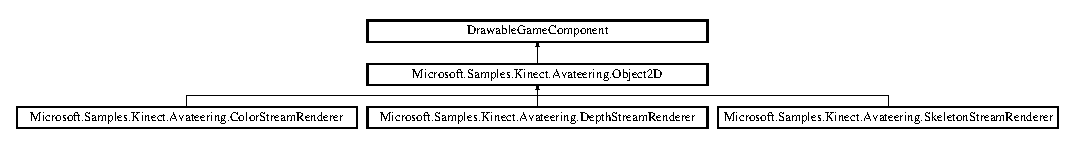
\includegraphics[height=1.501340cm]{class_microsoft_1_1_samples_1_1_kinect_1_1_avateering_1_1_object2_d}
\end{center}
\end{figure}
\subsection*{Public Member Functions}
\begin{DoxyCompactItemize}
\item 
\hyperlink{class_microsoft_1_1_samples_1_1_kinect_1_1_avateering_1_1_object2_d_af08680e0c439c7e69d808266fde543ec}{Object2\+D} (Game game)
\begin{DoxyCompactList}\small\item\em Initializes a new instance of the \hyperlink{class_microsoft_1_1_samples_1_1_kinect_1_1_avateering_1_1_object2_d}{Object2\+D} class. \end{DoxyCompactList}\end{DoxyCompactItemize}
\subsection*{Properties}
\begin{DoxyCompactItemize}
\item 
Vector2 \hyperlink{class_microsoft_1_1_samples_1_1_kinect_1_1_avateering_1_1_object2_d_a2ed3063bbd65e30889fda66d44eaec68}{Position}\hspace{0.3cm}{\ttfamily  \mbox{[}get, set\mbox{]}}
\begin{DoxyCompactList}\small\item\em Gets or sets the position of the object. \end{DoxyCompactList}\item 
Vector2 \hyperlink{class_microsoft_1_1_samples_1_1_kinect_1_1_avateering_1_1_object2_d_ac0f3198c3590593fe7b5d930ce1dab8b}{Size}\hspace{0.3cm}{\ttfamily  \mbox{[}get, set\mbox{]}}
\begin{DoxyCompactList}\small\item\em Gets or sets the size of the object. \end{DoxyCompactList}\item 
\hyperlink{class_microsoft_1_1_samples_1_1_kinect_1_1_avateering_1_1_kinect_chooser}{Kinect\+Chooser} \hyperlink{class_microsoft_1_1_samples_1_1_kinect_1_1_avateering_1_1_object2_d_af4e34597d808020610ffc9d148e5257e}{Chooser}\hspace{0.3cm}{\ttfamily  \mbox{[}get\mbox{]}}
\begin{DoxyCompactList}\small\item\em Gets the \hyperlink{class_microsoft_1_1_samples_1_1_kinect_1_1_avateering_1_1_kinect_chooser}{Kinect\+Chooser} from the services. \end{DoxyCompactList}\item 
\hypertarget{class_microsoft_1_1_samples_1_1_kinect_1_1_avateering_1_1_object2_d_a05ba44b27953eced5e78dbf77c6d4af4}{Sprite\+Batch {\bfseries Shared\+Sprite\+Batch}\hspace{0.3cm}{\ttfamily  \mbox{[}get\mbox{]}}}\label{class_microsoft_1_1_samples_1_1_kinect_1_1_avateering_1_1_object2_d_a05ba44b27953eced5e78dbf77c6d4af4}

\end{DoxyCompactItemize}


\subsection{Detailed Description}
A very basic game component to track common values. 



\subsection{Constructor \& Destructor Documentation}
\hypertarget{class_microsoft_1_1_samples_1_1_kinect_1_1_avateering_1_1_object2_d_af08680e0c439c7e69d808266fde543ec}{\index{Microsoft\+::\+Samples\+::\+Kinect\+::\+Avateering\+::\+Object2\+D@{Microsoft\+::\+Samples\+::\+Kinect\+::\+Avateering\+::\+Object2\+D}!Object2\+D@{Object2\+D}}
\index{Object2\+D@{Object2\+D}!Microsoft\+::\+Samples\+::\+Kinect\+::\+Avateering\+::\+Object2\+D@{Microsoft\+::\+Samples\+::\+Kinect\+::\+Avateering\+::\+Object2\+D}}
\subsubsection[{Object2\+D}]{\setlength{\rightskip}{0pt plus 5cm}Microsoft.\+Samples.\+Kinect.\+Avateering.\+Object2\+D.\+Object2\+D (
\begin{DoxyParamCaption}
\item[{Game}]{game}
\end{DoxyParamCaption}
)}}\label{class_microsoft_1_1_samples_1_1_kinect_1_1_avateering_1_1_object2_d_af08680e0c439c7e69d808266fde543ec}


Initializes a new instance of the \hyperlink{class_microsoft_1_1_samples_1_1_kinect_1_1_avateering_1_1_object2_d}{Object2\+D} class. 


\begin{DoxyParams}{Parameters}
{\em game} & The related game object.\\
\hline
\end{DoxyParams}


\subsection{Property Documentation}
\hypertarget{class_microsoft_1_1_samples_1_1_kinect_1_1_avateering_1_1_object2_d_af4e34597d808020610ffc9d148e5257e}{\index{Microsoft\+::\+Samples\+::\+Kinect\+::\+Avateering\+::\+Object2\+D@{Microsoft\+::\+Samples\+::\+Kinect\+::\+Avateering\+::\+Object2\+D}!Chooser@{Chooser}}
\index{Chooser@{Chooser}!Microsoft\+::\+Samples\+::\+Kinect\+::\+Avateering\+::\+Object2\+D@{Microsoft\+::\+Samples\+::\+Kinect\+::\+Avateering\+::\+Object2\+D}}
\subsubsection[{Chooser}]{\setlength{\rightskip}{0pt plus 5cm}{\bf Kinect\+Chooser} Microsoft.\+Samples.\+Kinect.\+Avateering.\+Object2\+D.\+Chooser\hspace{0.3cm}{\ttfamily [get]}}}\label{class_microsoft_1_1_samples_1_1_kinect_1_1_avateering_1_1_object2_d_af4e34597d808020610ffc9d148e5257e}


Gets the \hyperlink{class_microsoft_1_1_samples_1_1_kinect_1_1_avateering_1_1_kinect_chooser}{Kinect\+Chooser} from the services. 

\hypertarget{class_microsoft_1_1_samples_1_1_kinect_1_1_avateering_1_1_object2_d_a2ed3063bbd65e30889fda66d44eaec68}{\index{Microsoft\+::\+Samples\+::\+Kinect\+::\+Avateering\+::\+Object2\+D@{Microsoft\+::\+Samples\+::\+Kinect\+::\+Avateering\+::\+Object2\+D}!Position@{Position}}
\index{Position@{Position}!Microsoft\+::\+Samples\+::\+Kinect\+::\+Avateering\+::\+Object2\+D@{Microsoft\+::\+Samples\+::\+Kinect\+::\+Avateering\+::\+Object2\+D}}
\subsubsection[{Position}]{\setlength{\rightskip}{0pt plus 5cm}Vector2 Microsoft.\+Samples.\+Kinect.\+Avateering.\+Object2\+D.\+Position\hspace{0.3cm}{\ttfamily [get]}, {\ttfamily [set]}}}\label{class_microsoft_1_1_samples_1_1_kinect_1_1_avateering_1_1_object2_d_a2ed3063bbd65e30889fda66d44eaec68}


Gets or sets the position of the object. 

\hypertarget{class_microsoft_1_1_samples_1_1_kinect_1_1_avateering_1_1_object2_d_ac0f3198c3590593fe7b5d930ce1dab8b}{\index{Microsoft\+::\+Samples\+::\+Kinect\+::\+Avateering\+::\+Object2\+D@{Microsoft\+::\+Samples\+::\+Kinect\+::\+Avateering\+::\+Object2\+D}!Size@{Size}}
\index{Size@{Size}!Microsoft\+::\+Samples\+::\+Kinect\+::\+Avateering\+::\+Object2\+D@{Microsoft\+::\+Samples\+::\+Kinect\+::\+Avateering\+::\+Object2\+D}}
\subsubsection[{Size}]{\setlength{\rightskip}{0pt plus 5cm}Vector2 Microsoft.\+Samples.\+Kinect.\+Avateering.\+Object2\+D.\+Size\hspace{0.3cm}{\ttfamily [get]}, {\ttfamily [set]}}}\label{class_microsoft_1_1_samples_1_1_kinect_1_1_avateering_1_1_object2_d_ac0f3198c3590593fe7b5d930ce1dab8b}


Gets or sets the size of the object. 



The documentation for this class was generated from the following file\+:\begin{DoxyCompactItemize}
\item 
Avateering/Object2\+D.\+cs\end{DoxyCompactItemize}

\hypertarget{class_microsoft_1_1_samples_1_1_kinect_1_1_avateering_1_1_filters_1_1_skeleton_joints_filter_clipped_legs}{\section{Microsoft.\+Samples.\+Kinect.\+Avateering.\+Filters.\+Skeleton\+Joints\+Filter\+Clipped\+Legs Class Reference}
\label{class_microsoft_1_1_samples_1_1_kinect_1_1_avateering_1_1_filters_1_1_skeleton_joints_filter_clipped_legs}\index{Microsoft.\+Samples.\+Kinect.\+Avateering.\+Filters.\+Skeleton\+Joints\+Filter\+Clipped\+Legs@{Microsoft.\+Samples.\+Kinect.\+Avateering.\+Filters.\+Skeleton\+Joints\+Filter\+Clipped\+Legs}}
}


Filter\+Clipped\+Legs smooths out leg joint positions when the skeleton is clipped by the bottom of the camera F\+O\+V. Inferred joint positions from the skeletal tracker can occasionally be noisy or erroneous, based on limited depth image pixels from the parts of the legs in view. This filter applies a lot of smoothing using a double exponential filter, letting through just enough leg movement to show a kick or high step. Based on the amount of leg that is clipped/inferred, the smoothed data is feathered into the skeleton output data.  


\subsection*{Public Member Functions}
\begin{DoxyCompactItemize}
\item 
\hyperlink{class_microsoft_1_1_samples_1_1_kinect_1_1_avateering_1_1_filters_1_1_skeleton_joints_filter_clipped_legs_aef24b15a7f5d3d1229711af10c1c16f2}{Skeleton\+Joints\+Filter\+Clipped\+Legs} ()
\begin{DoxyCompactList}\small\item\em Initializes a new instance of the \hyperlink{class_microsoft_1_1_samples_1_1_kinect_1_1_avateering_1_1_filters_1_1_skeleton_joints_filter_clipped_legs}{Skeleton\+Joints\+Filter\+Clipped\+Legs} class. \end{DoxyCompactList}\item 
bool \hyperlink{class_microsoft_1_1_samples_1_1_kinect_1_1_avateering_1_1_filters_1_1_skeleton_joints_filter_clipped_legs_ab895f4113df237008e3f8f734c0a2919}{Filter\+Skeleton} (Skeleton skeleton, float delta\+Nui\+Time)
\begin{DoxyCompactList}\small\item\em Name\+: Filter\+Skeleton -\/ Implements the per-\/frame filter logic for the arms up patch. \end{DoxyCompactList}\item 
void \hyperlink{class_microsoft_1_1_samples_1_1_kinect_1_1_avateering_1_1_filters_1_1_skeleton_joints_filter_clipped_legs_a97c249e8768e13c5efbf8c87f33c5fe2}{Reset} ()
\begin{DoxyCompactList}\small\item\em Resets filter state to defaults. \end{DoxyCompactList}\end{DoxyCompactItemize}


\subsection{Detailed Description}
Filter\+Clipped\+Legs smooths out leg joint positions when the skeleton is clipped by the bottom of the camera F\+O\+V. Inferred joint positions from the skeletal tracker can occasionally be noisy or erroneous, based on limited depth image pixels from the parts of the legs in view. This filter applies a lot of smoothing using a double exponential filter, letting through just enough leg movement to show a kick or high step. Based on the amount of leg that is clipped/inferred, the smoothed data is feathered into the skeleton output data. 



\subsection{Constructor \& Destructor Documentation}
\hypertarget{class_microsoft_1_1_samples_1_1_kinect_1_1_avateering_1_1_filters_1_1_skeleton_joints_filter_clipped_legs_aef24b15a7f5d3d1229711af10c1c16f2}{\index{Microsoft\+::\+Samples\+::\+Kinect\+::\+Avateering\+::\+Filters\+::\+Skeleton\+Joints\+Filter\+Clipped\+Legs@{Microsoft\+::\+Samples\+::\+Kinect\+::\+Avateering\+::\+Filters\+::\+Skeleton\+Joints\+Filter\+Clipped\+Legs}!Skeleton\+Joints\+Filter\+Clipped\+Legs@{Skeleton\+Joints\+Filter\+Clipped\+Legs}}
\index{Skeleton\+Joints\+Filter\+Clipped\+Legs@{Skeleton\+Joints\+Filter\+Clipped\+Legs}!Microsoft\+::\+Samples\+::\+Kinect\+::\+Avateering\+::\+Filters\+::\+Skeleton\+Joints\+Filter\+Clipped\+Legs@{Microsoft\+::\+Samples\+::\+Kinect\+::\+Avateering\+::\+Filters\+::\+Skeleton\+Joints\+Filter\+Clipped\+Legs}}
\subsubsection[{Skeleton\+Joints\+Filter\+Clipped\+Legs}]{\setlength{\rightskip}{0pt plus 5cm}Microsoft.\+Samples.\+Kinect.\+Avateering.\+Filters.\+Skeleton\+Joints\+Filter\+Clipped\+Legs.\+Skeleton\+Joints\+Filter\+Clipped\+Legs (
\begin{DoxyParamCaption}
{}
\end{DoxyParamCaption}
)}}\label{class_microsoft_1_1_samples_1_1_kinect_1_1_avateering_1_1_filters_1_1_skeleton_joints_filter_clipped_legs_aef24b15a7f5d3d1229711af10c1c16f2}


Initializes a new instance of the \hyperlink{class_microsoft_1_1_samples_1_1_kinect_1_1_avateering_1_1_filters_1_1_skeleton_joints_filter_clipped_legs}{Skeleton\+Joints\+Filter\+Clipped\+Legs} class. 



\subsection{Member Function Documentation}
\hypertarget{class_microsoft_1_1_samples_1_1_kinect_1_1_avateering_1_1_filters_1_1_skeleton_joints_filter_clipped_legs_ab895f4113df237008e3f8f734c0a2919}{\index{Microsoft\+::\+Samples\+::\+Kinect\+::\+Avateering\+::\+Filters\+::\+Skeleton\+Joints\+Filter\+Clipped\+Legs@{Microsoft\+::\+Samples\+::\+Kinect\+::\+Avateering\+::\+Filters\+::\+Skeleton\+Joints\+Filter\+Clipped\+Legs}!Filter\+Skeleton@{Filter\+Skeleton}}
\index{Filter\+Skeleton@{Filter\+Skeleton}!Microsoft\+::\+Samples\+::\+Kinect\+::\+Avateering\+::\+Filters\+::\+Skeleton\+Joints\+Filter\+Clipped\+Legs@{Microsoft\+::\+Samples\+::\+Kinect\+::\+Avateering\+::\+Filters\+::\+Skeleton\+Joints\+Filter\+Clipped\+Legs}}
\subsubsection[{Filter\+Skeleton}]{\setlength{\rightskip}{0pt plus 5cm}bool Microsoft.\+Samples.\+Kinect.\+Avateering.\+Filters.\+Skeleton\+Joints\+Filter\+Clipped\+Legs.\+Filter\+Skeleton (
\begin{DoxyParamCaption}
\item[{Skeleton}]{skeleton, }
\item[{float}]{delta\+Nui\+Time}
\end{DoxyParamCaption}
)}}\label{class_microsoft_1_1_samples_1_1_kinect_1_1_avateering_1_1_filters_1_1_skeleton_joints_filter_clipped_legs_ab895f4113df237008e3f8f734c0a2919}


Name\+: Filter\+Skeleton -\/ Implements the per-\/frame filter logic for the arms up patch. 


\begin{DoxyParams}{Parameters}
{\em skeleton} & The skeleton to filter.\\
\hline
{\em delta\+Nui\+Time} & Time since the last filter update.\\
\hline
\end{DoxyParams}
\begin{DoxyReturn}{Returns}
Returns true if filter runs, false if it did not run.
\end{DoxyReturn}
\hypertarget{class_microsoft_1_1_samples_1_1_kinect_1_1_avateering_1_1_filters_1_1_skeleton_joints_filter_clipped_legs_a97c249e8768e13c5efbf8c87f33c5fe2}{\index{Microsoft\+::\+Samples\+::\+Kinect\+::\+Avateering\+::\+Filters\+::\+Skeleton\+Joints\+Filter\+Clipped\+Legs@{Microsoft\+::\+Samples\+::\+Kinect\+::\+Avateering\+::\+Filters\+::\+Skeleton\+Joints\+Filter\+Clipped\+Legs}!Reset@{Reset}}
\index{Reset@{Reset}!Microsoft\+::\+Samples\+::\+Kinect\+::\+Avateering\+::\+Filters\+::\+Skeleton\+Joints\+Filter\+Clipped\+Legs@{Microsoft\+::\+Samples\+::\+Kinect\+::\+Avateering\+::\+Filters\+::\+Skeleton\+Joints\+Filter\+Clipped\+Legs}}
\subsubsection[{Reset}]{\setlength{\rightskip}{0pt plus 5cm}void Microsoft.\+Samples.\+Kinect.\+Avateering.\+Filters.\+Skeleton\+Joints\+Filter\+Clipped\+Legs.\+Reset (
\begin{DoxyParamCaption}
{}
\end{DoxyParamCaption}
)}}\label{class_microsoft_1_1_samples_1_1_kinect_1_1_avateering_1_1_filters_1_1_skeleton_joints_filter_clipped_legs_a97c249e8768e13c5efbf8c87f33c5fe2}


Resets filter state to defaults. 



The documentation for this class was generated from the following file\+:\begin{DoxyCompactItemize}
\item 
Avateering/\+Filters/Skeleton\+Joints\+Filter\+Clipped\+Legs.\+cs\end{DoxyCompactItemize}

\hypertarget{class_microsoft_1_1_samples_1_1_kinect_1_1_avateering_1_1_filters_1_1_skeleton_joints_position_double_exponential_filter}{\section{Microsoft.\+Samples.\+Kinect.\+Avateering.\+Filters.\+Skeleton\+Joints\+Position\+Double\+Exponential\+Filter Class Reference}
\label{class_microsoft_1_1_samples_1_1_kinect_1_1_avateering_1_1_filters_1_1_skeleton_joints_position_double_exponential_filter}\index{Microsoft.\+Samples.\+Kinect.\+Avateering.\+Filters.\+Skeleton\+Joints\+Position\+Double\+Exponential\+Filter@{Microsoft.\+Samples.\+Kinect.\+Avateering.\+Filters.\+Skeleton\+Joints\+Position\+Double\+Exponential\+Filter}}
}


Implementation of a Holt Double Exponential Smoothing filter. The double exponential smooths the curve and predicts. There is also noise jitter removal. And maximum prediction bounds. The parameters are commented in the Init function.  


\subsection*{Public Member Functions}
\begin{DoxyCompactItemize}
\item 
\hyperlink{class_microsoft_1_1_samples_1_1_kinect_1_1_avateering_1_1_filters_1_1_skeleton_joints_position_double_exponential_filter_a115c464c8c6f81e223a1aa1382a3f378}{Skeleton\+Joints\+Position\+Double\+Exponential\+Filter} ()
\begin{DoxyCompactList}\small\item\em Initializes a new instance of the \hyperlink{class_microsoft_1_1_samples_1_1_kinect_1_1_avateering_1_1_filters_1_1_skeleton_joints_position_double_exponential_filter}{Skeleton\+Joints\+Position\+Double\+Exponential\+Filter} class. \end{DoxyCompactList}\item 
void \hyperlink{class_microsoft_1_1_samples_1_1_kinect_1_1_avateering_1_1_filters_1_1_skeleton_joints_position_double_exponential_filter_af77cac1895ff63de0a69d3306c06b00b}{Init} ()
\begin{DoxyCompactList}\small\item\em Initialize the filter with a default set of Transform\+Smooth\+Parameters. \end{DoxyCompactList}\item 
void \hyperlink{class_microsoft_1_1_samples_1_1_kinect_1_1_avateering_1_1_filters_1_1_skeleton_joints_position_double_exponential_filter_a72c4b893a04f0da0a00e7d76fe94a1ab}{Init} (float smoothing\+Value, float correction\+Value, float prediction\+Value, float jitter\+Radius\+Value, float max\+Deviation\+Radius\+Value)
\begin{DoxyCompactList}\small\item\em Initialize the filter with a set of manually specified Transform\+Smooth\+Parameters. \end{DoxyCompactList}\item 
void \hyperlink{class_microsoft_1_1_samples_1_1_kinect_1_1_avateering_1_1_filters_1_1_skeleton_joints_position_double_exponential_filter_ad4161509f17d4ee6809dd8d191dc2c56}{Init} (Transform\+Smooth\+Parameters smoothing\+Parameters)
\begin{DoxyCompactList}\small\item\em Initialize the filter with a set of Transform\+Smooth\+Parameters. \end{DoxyCompactList}\item 
void \hyperlink{class_microsoft_1_1_samples_1_1_kinect_1_1_avateering_1_1_filters_1_1_skeleton_joints_position_double_exponential_filter_a63907db70c589d23fe7302456ab58fe1}{Reset} ()
\begin{DoxyCompactList}\small\item\em Resets the filter to default values. \end{DoxyCompactList}\item 
void \hyperlink{class_microsoft_1_1_samples_1_1_kinect_1_1_avateering_1_1_filters_1_1_skeleton_joints_position_double_exponential_filter_a1853f70c62337ea0d07e4d590a06d5ab}{Update\+Filter} (Skeleton skeleton)
\begin{DoxyCompactList}\small\item\em Update the filter with a new frame of data and smooth. \end{DoxyCompactList}\end{DoxyCompactItemize}
\subsection*{Protected Member Functions}
\begin{DoxyCompactItemize}
\item 
void \hyperlink{class_microsoft_1_1_samples_1_1_kinect_1_1_avateering_1_1_filters_1_1_skeleton_joints_position_double_exponential_filter_acb576687a841dfb4d89b219bae4b6897}{Filter\+Joint} (Skeleton skeleton, Joint\+Type jt, Transform\+Smooth\+Parameters smoothing\+Parameters)
\begin{DoxyCompactList}\small\item\em Update the filter for one joint. \end{DoxyCompactList}\end{DoxyCompactItemize}


\subsection{Detailed Description}
Implementation of a Holt Double Exponential Smoothing filter. The double exponential smooths the curve and predicts. There is also noise jitter removal. And maximum prediction bounds. The parameters are commented in the Init function. 



\subsection{Constructor \& Destructor Documentation}
\hypertarget{class_microsoft_1_1_samples_1_1_kinect_1_1_avateering_1_1_filters_1_1_skeleton_joints_position_double_exponential_filter_a115c464c8c6f81e223a1aa1382a3f378}{\index{Microsoft\+::\+Samples\+::\+Kinect\+::\+Avateering\+::\+Filters\+::\+Skeleton\+Joints\+Position\+Double\+Exponential\+Filter@{Microsoft\+::\+Samples\+::\+Kinect\+::\+Avateering\+::\+Filters\+::\+Skeleton\+Joints\+Position\+Double\+Exponential\+Filter}!Skeleton\+Joints\+Position\+Double\+Exponential\+Filter@{Skeleton\+Joints\+Position\+Double\+Exponential\+Filter}}
\index{Skeleton\+Joints\+Position\+Double\+Exponential\+Filter@{Skeleton\+Joints\+Position\+Double\+Exponential\+Filter}!Microsoft\+::\+Samples\+::\+Kinect\+::\+Avateering\+::\+Filters\+::\+Skeleton\+Joints\+Position\+Double\+Exponential\+Filter@{Microsoft\+::\+Samples\+::\+Kinect\+::\+Avateering\+::\+Filters\+::\+Skeleton\+Joints\+Position\+Double\+Exponential\+Filter}}
\subsubsection[{Skeleton\+Joints\+Position\+Double\+Exponential\+Filter}]{\setlength{\rightskip}{0pt plus 5cm}Microsoft.\+Samples.\+Kinect.\+Avateering.\+Filters.\+Skeleton\+Joints\+Position\+Double\+Exponential\+Filter.\+Skeleton\+Joints\+Position\+Double\+Exponential\+Filter (
\begin{DoxyParamCaption}
{}
\end{DoxyParamCaption}
)}}\label{class_microsoft_1_1_samples_1_1_kinect_1_1_avateering_1_1_filters_1_1_skeleton_joints_position_double_exponential_filter_a115c464c8c6f81e223a1aa1382a3f378}


Initializes a new instance of the \hyperlink{class_microsoft_1_1_samples_1_1_kinect_1_1_avateering_1_1_filters_1_1_skeleton_joints_position_double_exponential_filter}{Skeleton\+Joints\+Position\+Double\+Exponential\+Filter} class. 



\subsection{Member Function Documentation}
\hypertarget{class_microsoft_1_1_samples_1_1_kinect_1_1_avateering_1_1_filters_1_1_skeleton_joints_position_double_exponential_filter_acb576687a841dfb4d89b219bae4b6897}{\index{Microsoft\+::\+Samples\+::\+Kinect\+::\+Avateering\+::\+Filters\+::\+Skeleton\+Joints\+Position\+Double\+Exponential\+Filter@{Microsoft\+::\+Samples\+::\+Kinect\+::\+Avateering\+::\+Filters\+::\+Skeleton\+Joints\+Position\+Double\+Exponential\+Filter}!Filter\+Joint@{Filter\+Joint}}
\index{Filter\+Joint@{Filter\+Joint}!Microsoft\+::\+Samples\+::\+Kinect\+::\+Avateering\+::\+Filters\+::\+Skeleton\+Joints\+Position\+Double\+Exponential\+Filter@{Microsoft\+::\+Samples\+::\+Kinect\+::\+Avateering\+::\+Filters\+::\+Skeleton\+Joints\+Position\+Double\+Exponential\+Filter}}
\subsubsection[{Filter\+Joint}]{\setlength{\rightskip}{0pt plus 5cm}void Microsoft.\+Samples.\+Kinect.\+Avateering.\+Filters.\+Skeleton\+Joints\+Position\+Double\+Exponential\+Filter.\+Filter\+Joint (
\begin{DoxyParamCaption}
\item[{Skeleton}]{skeleton, }
\item[{Joint\+Type}]{jt, }
\item[{Transform\+Smooth\+Parameters}]{smoothing\+Parameters}
\end{DoxyParamCaption}
)\hspace{0.3cm}{\ttfamily [protected]}}}\label{class_microsoft_1_1_samples_1_1_kinect_1_1_avateering_1_1_filters_1_1_skeleton_joints_position_double_exponential_filter_acb576687a841dfb4d89b219bae4b6897}


Update the filter for one joint. 


\begin{DoxyParams}{Parameters}
{\em skeleton} & The Skeleton to filter.\\
\hline
{\em jt} & The Skeleton Joint index to filter.\\
\hline
{\em smoothing\+Parameters} & The Smoothing parameters to apply.\\
\hline
\end{DoxyParams}
\hypertarget{class_microsoft_1_1_samples_1_1_kinect_1_1_avateering_1_1_filters_1_1_skeleton_joints_position_double_exponential_filter_af77cac1895ff63de0a69d3306c06b00b}{\index{Microsoft\+::\+Samples\+::\+Kinect\+::\+Avateering\+::\+Filters\+::\+Skeleton\+Joints\+Position\+Double\+Exponential\+Filter@{Microsoft\+::\+Samples\+::\+Kinect\+::\+Avateering\+::\+Filters\+::\+Skeleton\+Joints\+Position\+Double\+Exponential\+Filter}!Init@{Init}}
\index{Init@{Init}!Microsoft\+::\+Samples\+::\+Kinect\+::\+Avateering\+::\+Filters\+::\+Skeleton\+Joints\+Position\+Double\+Exponential\+Filter@{Microsoft\+::\+Samples\+::\+Kinect\+::\+Avateering\+::\+Filters\+::\+Skeleton\+Joints\+Position\+Double\+Exponential\+Filter}}
\subsubsection[{Init}]{\setlength{\rightskip}{0pt plus 5cm}void Microsoft.\+Samples.\+Kinect.\+Avateering.\+Filters.\+Skeleton\+Joints\+Position\+Double\+Exponential\+Filter.\+Init (
\begin{DoxyParamCaption}
{}
\end{DoxyParamCaption}
)}}\label{class_microsoft_1_1_samples_1_1_kinect_1_1_avateering_1_1_filters_1_1_skeleton_joints_position_double_exponential_filter_af77cac1895ff63de0a69d3306c06b00b}


Initialize the filter with a default set of Transform\+Smooth\+Parameters. 

\hypertarget{class_microsoft_1_1_samples_1_1_kinect_1_1_avateering_1_1_filters_1_1_skeleton_joints_position_double_exponential_filter_a72c4b893a04f0da0a00e7d76fe94a1ab}{\index{Microsoft\+::\+Samples\+::\+Kinect\+::\+Avateering\+::\+Filters\+::\+Skeleton\+Joints\+Position\+Double\+Exponential\+Filter@{Microsoft\+::\+Samples\+::\+Kinect\+::\+Avateering\+::\+Filters\+::\+Skeleton\+Joints\+Position\+Double\+Exponential\+Filter}!Init@{Init}}
\index{Init@{Init}!Microsoft\+::\+Samples\+::\+Kinect\+::\+Avateering\+::\+Filters\+::\+Skeleton\+Joints\+Position\+Double\+Exponential\+Filter@{Microsoft\+::\+Samples\+::\+Kinect\+::\+Avateering\+::\+Filters\+::\+Skeleton\+Joints\+Position\+Double\+Exponential\+Filter}}
\subsubsection[{Init}]{\setlength{\rightskip}{0pt plus 5cm}void Microsoft.\+Samples.\+Kinect.\+Avateering.\+Filters.\+Skeleton\+Joints\+Position\+Double\+Exponential\+Filter.\+Init (
\begin{DoxyParamCaption}
\item[{float}]{smoothing\+Value, }
\item[{float}]{correction\+Value, }
\item[{float}]{prediction\+Value, }
\item[{float}]{jitter\+Radius\+Value, }
\item[{float}]{max\+Deviation\+Radius\+Value}
\end{DoxyParamCaption}
)}}\label{class_microsoft_1_1_samples_1_1_kinect_1_1_avateering_1_1_filters_1_1_skeleton_joints_position_double_exponential_filter_a72c4b893a04f0da0a00e7d76fe94a1ab}


Initialize the filter with a set of manually specified Transform\+Smooth\+Parameters. 


\begin{DoxyParams}{Parameters}
{\em smoothing\+Value} & Smoothing = \mbox{[}0..1\mbox{]}, lower values is closer to the raw data and more noisy.\\
\hline
{\em correction\+Value} & Correction = \mbox{[}0..1\mbox{]}, higher values correct faster and feel more responsive.\\
\hline
{\em prediction\+Value} & Prediction = \mbox{[}0..n\mbox{]}, how many frames into the future we want to predict.\\
\hline
{\em jitter\+Radius\+Value} & Jitter\+Radius = The deviation distance in m that defines jitter.\\
\hline
{\em max\+Deviation\+Radius\+Value} & Max\+Deviation = The maximum distance in m that filtered positions are allowed to deviate from raw data.\\
\hline
\end{DoxyParams}
\hypertarget{class_microsoft_1_1_samples_1_1_kinect_1_1_avateering_1_1_filters_1_1_skeleton_joints_position_double_exponential_filter_ad4161509f17d4ee6809dd8d191dc2c56}{\index{Microsoft\+::\+Samples\+::\+Kinect\+::\+Avateering\+::\+Filters\+::\+Skeleton\+Joints\+Position\+Double\+Exponential\+Filter@{Microsoft\+::\+Samples\+::\+Kinect\+::\+Avateering\+::\+Filters\+::\+Skeleton\+Joints\+Position\+Double\+Exponential\+Filter}!Init@{Init}}
\index{Init@{Init}!Microsoft\+::\+Samples\+::\+Kinect\+::\+Avateering\+::\+Filters\+::\+Skeleton\+Joints\+Position\+Double\+Exponential\+Filter@{Microsoft\+::\+Samples\+::\+Kinect\+::\+Avateering\+::\+Filters\+::\+Skeleton\+Joints\+Position\+Double\+Exponential\+Filter}}
\subsubsection[{Init}]{\setlength{\rightskip}{0pt plus 5cm}void Microsoft.\+Samples.\+Kinect.\+Avateering.\+Filters.\+Skeleton\+Joints\+Position\+Double\+Exponential\+Filter.\+Init (
\begin{DoxyParamCaption}
\item[{Transform\+Smooth\+Parameters}]{smoothing\+Parameters}
\end{DoxyParamCaption}
)}}\label{class_microsoft_1_1_samples_1_1_kinect_1_1_avateering_1_1_filters_1_1_skeleton_joints_position_double_exponential_filter_ad4161509f17d4ee6809dd8d191dc2c56}


Initialize the filter with a set of Transform\+Smooth\+Parameters. 


\begin{DoxyParams}{Parameters}
{\em smoothing\+Parameters} & The smoothing parameters to filter with.\\
\hline
\end{DoxyParams}
\hypertarget{class_microsoft_1_1_samples_1_1_kinect_1_1_avateering_1_1_filters_1_1_skeleton_joints_position_double_exponential_filter_a63907db70c589d23fe7302456ab58fe1}{\index{Microsoft\+::\+Samples\+::\+Kinect\+::\+Avateering\+::\+Filters\+::\+Skeleton\+Joints\+Position\+Double\+Exponential\+Filter@{Microsoft\+::\+Samples\+::\+Kinect\+::\+Avateering\+::\+Filters\+::\+Skeleton\+Joints\+Position\+Double\+Exponential\+Filter}!Reset@{Reset}}
\index{Reset@{Reset}!Microsoft\+::\+Samples\+::\+Kinect\+::\+Avateering\+::\+Filters\+::\+Skeleton\+Joints\+Position\+Double\+Exponential\+Filter@{Microsoft\+::\+Samples\+::\+Kinect\+::\+Avateering\+::\+Filters\+::\+Skeleton\+Joints\+Position\+Double\+Exponential\+Filter}}
\subsubsection[{Reset}]{\setlength{\rightskip}{0pt plus 5cm}void Microsoft.\+Samples.\+Kinect.\+Avateering.\+Filters.\+Skeleton\+Joints\+Position\+Double\+Exponential\+Filter.\+Reset (
\begin{DoxyParamCaption}
{}
\end{DoxyParamCaption}
)}}\label{class_microsoft_1_1_samples_1_1_kinect_1_1_avateering_1_1_filters_1_1_skeleton_joints_position_double_exponential_filter_a63907db70c589d23fe7302456ab58fe1}


Resets the filter to default values. 

\hypertarget{class_microsoft_1_1_samples_1_1_kinect_1_1_avateering_1_1_filters_1_1_skeleton_joints_position_double_exponential_filter_a1853f70c62337ea0d07e4d590a06d5ab}{\index{Microsoft\+::\+Samples\+::\+Kinect\+::\+Avateering\+::\+Filters\+::\+Skeleton\+Joints\+Position\+Double\+Exponential\+Filter@{Microsoft\+::\+Samples\+::\+Kinect\+::\+Avateering\+::\+Filters\+::\+Skeleton\+Joints\+Position\+Double\+Exponential\+Filter}!Update\+Filter@{Update\+Filter}}
\index{Update\+Filter@{Update\+Filter}!Microsoft\+::\+Samples\+::\+Kinect\+::\+Avateering\+::\+Filters\+::\+Skeleton\+Joints\+Position\+Double\+Exponential\+Filter@{Microsoft\+::\+Samples\+::\+Kinect\+::\+Avateering\+::\+Filters\+::\+Skeleton\+Joints\+Position\+Double\+Exponential\+Filter}}
\subsubsection[{Update\+Filter}]{\setlength{\rightskip}{0pt plus 5cm}void Microsoft.\+Samples.\+Kinect.\+Avateering.\+Filters.\+Skeleton\+Joints\+Position\+Double\+Exponential\+Filter.\+Update\+Filter (
\begin{DoxyParamCaption}
\item[{Skeleton}]{skeleton}
\end{DoxyParamCaption}
)}}\label{class_microsoft_1_1_samples_1_1_kinect_1_1_avateering_1_1_filters_1_1_skeleton_joints_position_double_exponential_filter_a1853f70c62337ea0d07e4d590a06d5ab}


Update the filter with a new frame of data and smooth. 


\begin{DoxyParams}{Parameters}
{\em skeleton} & The Skeleton to filter.\\
\hline
\end{DoxyParams}


The documentation for this class was generated from the following file\+:\begin{DoxyCompactItemize}
\item 
Avateering/\+Filters/Skeleton\+Joints\+Position\+Double\+Exponential\+Filter.\+cs\end{DoxyCompactItemize}

\hypertarget{class_microsoft_1_1_samples_1_1_kinect_1_1_avateering_1_1_filters_1_1_skeleton_joints_sensor_offset_correction}{\section{Microsoft.\+Samples.\+Kinect.\+Avateering.\+Filters.\+Skeleton\+Joints\+Sensor\+Offset\+Correction Class Reference}
\label{class_microsoft_1_1_samples_1_1_kinect_1_1_avateering_1_1_filters_1_1_skeleton_joints_sensor_offset_correction}\index{Microsoft.\+Samples.\+Kinect.\+Avateering.\+Filters.\+Skeleton\+Joints\+Sensor\+Offset\+Correction@{Microsoft.\+Samples.\+Kinect.\+Avateering.\+Filters.\+Skeleton\+Joints\+Sensor\+Offset\+Correction}}
}


Filter to correct the skeleton position for the sensor height above the floor, to enable an avatar to be placed with feet on the ground plane.  


\subsection*{Public Member Functions}
\begin{DoxyCompactItemize}
\item 
\hyperlink{class_microsoft_1_1_samples_1_1_kinect_1_1_avateering_1_1_filters_1_1_skeleton_joints_sensor_offset_correction_a0a219f1b8a9f7702a7965c64dfd84a6b}{Skeleton\+Joints\+Sensor\+Offset\+Correction} ()
\begin{DoxyCompactList}\small\item\em Initializes a new instance of the \hyperlink{class_microsoft_1_1_samples_1_1_kinect_1_1_avateering_1_1_filters_1_1_skeleton_joints_sensor_offset_correction}{Skeleton\+Joints\+Sensor\+Offset\+Correction} class. \end{DoxyCompactList}\item 
void \hyperlink{class_microsoft_1_1_samples_1_1_kinect_1_1_avateering_1_1_filters_1_1_skeleton_joints_sensor_offset_correction_a58aa2a575cf71b7b51ebdc8a6c156175}{Reset} ()
\begin{DoxyCompactList}\small\item\em Resets the average floor offset. \end{DoxyCompactList}\item 
void \hyperlink{class_microsoft_1_1_samples_1_1_kinect_1_1_avateering_1_1_filters_1_1_skeleton_joints_sensor_offset_correction_a878127fb5ec53cefbfd76e9afef34952}{Correct\+Skeleton\+Offset\+From\+Floor} (Skeleton skeleton, Tuple$<$ float, float, float, float $>$ floor\+Plane, float avatar\+Hip\+Center\+Height)
\begin{DoxyCompactList}\small\item\em Correct\+Skeleton\+Offset\+From\+Floor moves the skeleton to the floor. If no floor found in Skeletal Tracking, we can try and use the foot position but this can be very noisy, which causes the skeleton to bounce up and down. Note\+: Using the foot positions will reduce the visual effect of jumping when an avateer jumps, as we perform a running average. \end{DoxyCompactList}\end{DoxyCompactItemize}


\subsection{Detailed Description}
Filter to correct the skeleton position for the sensor height above the floor, to enable an avatar to be placed with feet on the ground plane. 



\subsection{Constructor \& Destructor Documentation}
\hypertarget{class_microsoft_1_1_samples_1_1_kinect_1_1_avateering_1_1_filters_1_1_skeleton_joints_sensor_offset_correction_a0a219f1b8a9f7702a7965c64dfd84a6b}{\index{Microsoft\+::\+Samples\+::\+Kinect\+::\+Avateering\+::\+Filters\+::\+Skeleton\+Joints\+Sensor\+Offset\+Correction@{Microsoft\+::\+Samples\+::\+Kinect\+::\+Avateering\+::\+Filters\+::\+Skeleton\+Joints\+Sensor\+Offset\+Correction}!Skeleton\+Joints\+Sensor\+Offset\+Correction@{Skeleton\+Joints\+Sensor\+Offset\+Correction}}
\index{Skeleton\+Joints\+Sensor\+Offset\+Correction@{Skeleton\+Joints\+Sensor\+Offset\+Correction}!Microsoft\+::\+Samples\+::\+Kinect\+::\+Avateering\+::\+Filters\+::\+Skeleton\+Joints\+Sensor\+Offset\+Correction@{Microsoft\+::\+Samples\+::\+Kinect\+::\+Avateering\+::\+Filters\+::\+Skeleton\+Joints\+Sensor\+Offset\+Correction}}
\subsubsection[{Skeleton\+Joints\+Sensor\+Offset\+Correction}]{\setlength{\rightskip}{0pt plus 5cm}Microsoft.\+Samples.\+Kinect.\+Avateering.\+Filters.\+Skeleton\+Joints\+Sensor\+Offset\+Correction.\+Skeleton\+Joints\+Sensor\+Offset\+Correction (
\begin{DoxyParamCaption}
{}
\end{DoxyParamCaption}
)}}\label{class_microsoft_1_1_samples_1_1_kinect_1_1_avateering_1_1_filters_1_1_skeleton_joints_sensor_offset_correction_a0a219f1b8a9f7702a7965c64dfd84a6b}


Initializes a new instance of the \hyperlink{class_microsoft_1_1_samples_1_1_kinect_1_1_avateering_1_1_filters_1_1_skeleton_joints_sensor_offset_correction}{Skeleton\+Joints\+Sensor\+Offset\+Correction} class. 



\subsection{Member Function Documentation}
\hypertarget{class_microsoft_1_1_samples_1_1_kinect_1_1_avateering_1_1_filters_1_1_skeleton_joints_sensor_offset_correction_a878127fb5ec53cefbfd76e9afef34952}{\index{Microsoft\+::\+Samples\+::\+Kinect\+::\+Avateering\+::\+Filters\+::\+Skeleton\+Joints\+Sensor\+Offset\+Correction@{Microsoft\+::\+Samples\+::\+Kinect\+::\+Avateering\+::\+Filters\+::\+Skeleton\+Joints\+Sensor\+Offset\+Correction}!Correct\+Skeleton\+Offset\+From\+Floor@{Correct\+Skeleton\+Offset\+From\+Floor}}
\index{Correct\+Skeleton\+Offset\+From\+Floor@{Correct\+Skeleton\+Offset\+From\+Floor}!Microsoft\+::\+Samples\+::\+Kinect\+::\+Avateering\+::\+Filters\+::\+Skeleton\+Joints\+Sensor\+Offset\+Correction@{Microsoft\+::\+Samples\+::\+Kinect\+::\+Avateering\+::\+Filters\+::\+Skeleton\+Joints\+Sensor\+Offset\+Correction}}
\subsubsection[{Correct\+Skeleton\+Offset\+From\+Floor}]{\setlength{\rightskip}{0pt plus 5cm}void Microsoft.\+Samples.\+Kinect.\+Avateering.\+Filters.\+Skeleton\+Joints\+Sensor\+Offset\+Correction.\+Correct\+Skeleton\+Offset\+From\+Floor (
\begin{DoxyParamCaption}
\item[{Skeleton}]{skeleton, }
\item[{Tuple$<$ float, float, float, float $>$}]{floor\+Plane, }
\item[{float}]{avatar\+Hip\+Center\+Height}
\end{DoxyParamCaption}
)}}\label{class_microsoft_1_1_samples_1_1_kinect_1_1_avateering_1_1_filters_1_1_skeleton_joints_sensor_offset_correction_a878127fb5ec53cefbfd76e9afef34952}


Correct\+Skeleton\+Offset\+From\+Floor moves the skeleton to the floor. If no floor found in Skeletal Tracking, we can try and use the foot position but this can be very noisy, which causes the skeleton to bounce up and down. Note\+: Using the foot positions will reduce the visual effect of jumping when an avateer jumps, as we perform a running average. 


\begin{DoxyParams}{Parameters}
{\em skeleton} & The skeleton to correct.\\
\hline
{\em floor\+Plane} & The floor plane (consisting of up normal and sensor height) detected by skeleton tracking (if any).\\
\hline
{\em avatar\+Hip\+Center\+Height} & The height of the avatar Hip Center joint.\\
\hline
\end{DoxyParams}
\hypertarget{class_microsoft_1_1_samples_1_1_kinect_1_1_avateering_1_1_filters_1_1_skeleton_joints_sensor_offset_correction_a58aa2a575cf71b7b51ebdc8a6c156175}{\index{Microsoft\+::\+Samples\+::\+Kinect\+::\+Avateering\+::\+Filters\+::\+Skeleton\+Joints\+Sensor\+Offset\+Correction@{Microsoft\+::\+Samples\+::\+Kinect\+::\+Avateering\+::\+Filters\+::\+Skeleton\+Joints\+Sensor\+Offset\+Correction}!Reset@{Reset}}
\index{Reset@{Reset}!Microsoft\+::\+Samples\+::\+Kinect\+::\+Avateering\+::\+Filters\+::\+Skeleton\+Joints\+Sensor\+Offset\+Correction@{Microsoft\+::\+Samples\+::\+Kinect\+::\+Avateering\+::\+Filters\+::\+Skeleton\+Joints\+Sensor\+Offset\+Correction}}
\subsubsection[{Reset}]{\setlength{\rightskip}{0pt plus 5cm}void Microsoft.\+Samples.\+Kinect.\+Avateering.\+Filters.\+Skeleton\+Joints\+Sensor\+Offset\+Correction.\+Reset (
\begin{DoxyParamCaption}
{}
\end{DoxyParamCaption}
)}}\label{class_microsoft_1_1_samples_1_1_kinect_1_1_avateering_1_1_filters_1_1_skeleton_joints_sensor_offset_correction_a58aa2a575cf71b7b51ebdc8a6c156175}


Resets the average floor offset. 



The documentation for this class was generated from the following file\+:\begin{DoxyCompactItemize}
\item 
Avateering/\+Filters/Skeleton\+Joints\+Sensor\+Offset\+Correction.\+cs\end{DoxyCompactItemize}

\hypertarget{class_microsoft_1_1_samples_1_1_kinect_1_1_avateering_1_1_skeleton_stream_renderer}{\section{Microsoft.\+Samples.\+Kinect.\+Avateering.\+Skeleton\+Stream\+Renderer Class Reference}
\label{class_microsoft_1_1_samples_1_1_kinect_1_1_avateering_1_1_skeleton_stream_renderer}\index{Microsoft.\+Samples.\+Kinect.\+Avateering.\+Skeleton\+Stream\+Renderer@{Microsoft.\+Samples.\+Kinect.\+Avateering.\+Skeleton\+Stream\+Renderer}}
}


This class is responsible for rendering a skeleton stream.  


Inheritance diagram for Microsoft.\+Samples.\+Kinect.\+Avateering.\+Skeleton\+Stream\+Renderer\+:\begin{figure}[H]
\begin{center}
\leavevmode
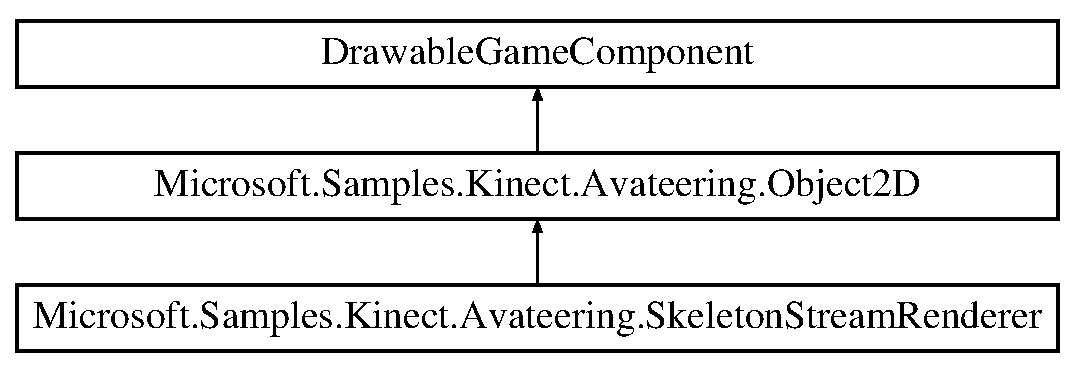
\includegraphics[height=3.000000cm]{class_microsoft_1_1_samples_1_1_kinect_1_1_avateering_1_1_skeleton_stream_renderer}
\end{center}
\end{figure}
\subsection*{Public Member Functions}
\begin{DoxyCompactItemize}
\item 
\hyperlink{class_microsoft_1_1_samples_1_1_kinect_1_1_avateering_1_1_skeleton_stream_renderer_af0974bf772920b91479aab6a2038ec8c}{Skeleton\+Stream\+Renderer} (Game game, \hyperlink{namespace_microsoft_1_1_samples_1_1_kinect_1_1_avateering_ae8146e6f856d793f4fe4030a7a50a9d1}{Skeleton\+Point\+Map} map)
\begin{DoxyCompactList}\small\item\em Initializes a new instance of the \hyperlink{class_microsoft_1_1_samples_1_1_kinect_1_1_avateering_1_1_skeleton_stream_renderer}{Skeleton\+Stream\+Renderer} class. \end{DoxyCompactList}\item 
override void \hyperlink{class_microsoft_1_1_samples_1_1_kinect_1_1_avateering_1_1_skeleton_stream_renderer_af47e90f667253a9c1bd3116f607c69fd}{Initialize} ()
\begin{DoxyCompactList}\small\item\em This method initializes necessary values. \end{DoxyCompactList}\item 
void \hyperlink{class_microsoft_1_1_samples_1_1_kinect_1_1_avateering_1_1_skeleton_stream_renderer_a9beca14a74f9e496756a97f828364149}{Update} (Game\+Time game\+Time, Skeleton\mbox{[}$\,$\mbox{]} skeleton\+Frame\+Data)
\begin{DoxyCompactList}\small\item\em This method retrieves a new skeleton frame if necessary. \end{DoxyCompactList}\item 
override void \hyperlink{class_microsoft_1_1_samples_1_1_kinect_1_1_avateering_1_1_skeleton_stream_renderer_a3c07b064603a3a47dbcd968b9972e41d}{Draw} (Game\+Time game\+Time)
\begin{DoxyCompactList}\small\item\em This method draws the skeleton frame data. \end{DoxyCompactList}\end{DoxyCompactItemize}
\subsection*{Protected Member Functions}
\begin{DoxyCompactItemize}
\item 
override void \hyperlink{class_microsoft_1_1_samples_1_1_kinect_1_1_avateering_1_1_skeleton_stream_renderer_abc25b8c3f2cb598c5c4e59b9dbea1785}{Load\+Content} ()
\begin{DoxyCompactList}\small\item\em This method loads the textures and sets the origin values. \end{DoxyCompactList}\end{DoxyCompactItemize}
\subsection*{Properties}
\begin{DoxyCompactItemize}
\item 
Sprite\+Batch \hyperlink{class_microsoft_1_1_samples_1_1_kinect_1_1_avateering_1_1_skeleton_stream_renderer_af2e495e28c265c1dfb7797d89e16e06e}{Shared\+Sprite\+Batch}\hspace{0.3cm}{\ttfamily  \mbox{[}get\mbox{]}}
\begin{DoxyCompactList}\small\item\em Gets the Sprite\+Batch from the services. \end{DoxyCompactList}\end{DoxyCompactItemize}


\subsection{Detailed Description}
This class is responsible for rendering a skeleton stream. 



\subsection{Constructor \& Destructor Documentation}
\hypertarget{class_microsoft_1_1_samples_1_1_kinect_1_1_avateering_1_1_skeleton_stream_renderer_af0974bf772920b91479aab6a2038ec8c}{\index{Microsoft\+::\+Samples\+::\+Kinect\+::\+Avateering\+::\+Skeleton\+Stream\+Renderer@{Microsoft\+::\+Samples\+::\+Kinect\+::\+Avateering\+::\+Skeleton\+Stream\+Renderer}!Skeleton\+Stream\+Renderer@{Skeleton\+Stream\+Renderer}}
\index{Skeleton\+Stream\+Renderer@{Skeleton\+Stream\+Renderer}!Microsoft\+::\+Samples\+::\+Kinect\+::\+Avateering\+::\+Skeleton\+Stream\+Renderer@{Microsoft\+::\+Samples\+::\+Kinect\+::\+Avateering\+::\+Skeleton\+Stream\+Renderer}}
\subsubsection[{Skeleton\+Stream\+Renderer}]{\setlength{\rightskip}{0pt plus 5cm}Microsoft.\+Samples.\+Kinect.\+Avateering.\+Skeleton\+Stream\+Renderer.\+Skeleton\+Stream\+Renderer (
\begin{DoxyParamCaption}
\item[{Game}]{game, }
\item[{{\bf Skeleton\+Point\+Map}}]{map}
\end{DoxyParamCaption}
)}}\label{class_microsoft_1_1_samples_1_1_kinect_1_1_avateering_1_1_skeleton_stream_renderer_af0974bf772920b91479aab6a2038ec8c}


Initializes a new instance of the \hyperlink{class_microsoft_1_1_samples_1_1_kinect_1_1_avateering_1_1_skeleton_stream_renderer}{Skeleton\+Stream\+Renderer} class. 


\begin{DoxyParams}{Parameters}
{\em game} & The related game object.\\
\hline
{\em map} & The method used to map the Skeleton\+Point to the target space.\\
\hline
\end{DoxyParams}


\subsection{Member Function Documentation}
\hypertarget{class_microsoft_1_1_samples_1_1_kinect_1_1_avateering_1_1_skeleton_stream_renderer_a3c07b064603a3a47dbcd968b9972e41d}{\index{Microsoft\+::\+Samples\+::\+Kinect\+::\+Avateering\+::\+Skeleton\+Stream\+Renderer@{Microsoft\+::\+Samples\+::\+Kinect\+::\+Avateering\+::\+Skeleton\+Stream\+Renderer}!Draw@{Draw}}
\index{Draw@{Draw}!Microsoft\+::\+Samples\+::\+Kinect\+::\+Avateering\+::\+Skeleton\+Stream\+Renderer@{Microsoft\+::\+Samples\+::\+Kinect\+::\+Avateering\+::\+Skeleton\+Stream\+Renderer}}
\subsubsection[{Draw}]{\setlength{\rightskip}{0pt plus 5cm}override void Microsoft.\+Samples.\+Kinect.\+Avateering.\+Skeleton\+Stream\+Renderer.\+Draw (
\begin{DoxyParamCaption}
\item[{Game\+Time}]{game\+Time}
\end{DoxyParamCaption}
)}}\label{class_microsoft_1_1_samples_1_1_kinect_1_1_avateering_1_1_skeleton_stream_renderer_a3c07b064603a3a47dbcd968b9972e41d}


This method draws the skeleton frame data. 


\begin{DoxyParams}{Parameters}
{\em game\+Time} & The elapsed game time.\\
\hline
\end{DoxyParams}
\hypertarget{class_microsoft_1_1_samples_1_1_kinect_1_1_avateering_1_1_skeleton_stream_renderer_af47e90f667253a9c1bd3116f607c69fd}{\index{Microsoft\+::\+Samples\+::\+Kinect\+::\+Avateering\+::\+Skeleton\+Stream\+Renderer@{Microsoft\+::\+Samples\+::\+Kinect\+::\+Avateering\+::\+Skeleton\+Stream\+Renderer}!Initialize@{Initialize}}
\index{Initialize@{Initialize}!Microsoft\+::\+Samples\+::\+Kinect\+::\+Avateering\+::\+Skeleton\+Stream\+Renderer@{Microsoft\+::\+Samples\+::\+Kinect\+::\+Avateering\+::\+Skeleton\+Stream\+Renderer}}
\subsubsection[{Initialize}]{\setlength{\rightskip}{0pt plus 5cm}override void Microsoft.\+Samples.\+Kinect.\+Avateering.\+Skeleton\+Stream\+Renderer.\+Initialize (
\begin{DoxyParamCaption}
{}
\end{DoxyParamCaption}
)}}\label{class_microsoft_1_1_samples_1_1_kinect_1_1_avateering_1_1_skeleton_stream_renderer_af47e90f667253a9c1bd3116f607c69fd}


This method initializes necessary values. 

\hypertarget{class_microsoft_1_1_samples_1_1_kinect_1_1_avateering_1_1_skeleton_stream_renderer_abc25b8c3f2cb598c5c4e59b9dbea1785}{\index{Microsoft\+::\+Samples\+::\+Kinect\+::\+Avateering\+::\+Skeleton\+Stream\+Renderer@{Microsoft\+::\+Samples\+::\+Kinect\+::\+Avateering\+::\+Skeleton\+Stream\+Renderer}!Load\+Content@{Load\+Content}}
\index{Load\+Content@{Load\+Content}!Microsoft\+::\+Samples\+::\+Kinect\+::\+Avateering\+::\+Skeleton\+Stream\+Renderer@{Microsoft\+::\+Samples\+::\+Kinect\+::\+Avateering\+::\+Skeleton\+Stream\+Renderer}}
\subsubsection[{Load\+Content}]{\setlength{\rightskip}{0pt plus 5cm}override void Microsoft.\+Samples.\+Kinect.\+Avateering.\+Skeleton\+Stream\+Renderer.\+Load\+Content (
\begin{DoxyParamCaption}
{}
\end{DoxyParamCaption}
)\hspace{0.3cm}{\ttfamily [protected]}}}\label{class_microsoft_1_1_samples_1_1_kinect_1_1_avateering_1_1_skeleton_stream_renderer_abc25b8c3f2cb598c5c4e59b9dbea1785}


This method loads the textures and sets the origin values. 

\hypertarget{class_microsoft_1_1_samples_1_1_kinect_1_1_avateering_1_1_skeleton_stream_renderer_a9beca14a74f9e496756a97f828364149}{\index{Microsoft\+::\+Samples\+::\+Kinect\+::\+Avateering\+::\+Skeleton\+Stream\+Renderer@{Microsoft\+::\+Samples\+::\+Kinect\+::\+Avateering\+::\+Skeleton\+Stream\+Renderer}!Update@{Update}}
\index{Update@{Update}!Microsoft\+::\+Samples\+::\+Kinect\+::\+Avateering\+::\+Skeleton\+Stream\+Renderer@{Microsoft\+::\+Samples\+::\+Kinect\+::\+Avateering\+::\+Skeleton\+Stream\+Renderer}}
\subsubsection[{Update}]{\setlength{\rightskip}{0pt plus 5cm}void Microsoft.\+Samples.\+Kinect.\+Avateering.\+Skeleton\+Stream\+Renderer.\+Update (
\begin{DoxyParamCaption}
\item[{Game\+Time}]{game\+Time, }
\item[{Skeleton\mbox{[}$\,$\mbox{]}}]{skeleton\+Frame\+Data}
\end{DoxyParamCaption}
)}}\label{class_microsoft_1_1_samples_1_1_kinect_1_1_avateering_1_1_skeleton_stream_renderer_a9beca14a74f9e496756a97f828364149}


This method retrieves a new skeleton frame if necessary. 


\begin{DoxyParams}{Parameters}
{\em game\+Time} & The elapsed game time.\\
\hline
{\em skeleton\+Frame\+Data} & The skeleton data for the current frame.\\
\hline
\end{DoxyParams}


\subsection{Property Documentation}
\hypertarget{class_microsoft_1_1_samples_1_1_kinect_1_1_avateering_1_1_skeleton_stream_renderer_af2e495e28c265c1dfb7797d89e16e06e}{\index{Microsoft\+::\+Samples\+::\+Kinect\+::\+Avateering\+::\+Skeleton\+Stream\+Renderer@{Microsoft\+::\+Samples\+::\+Kinect\+::\+Avateering\+::\+Skeleton\+Stream\+Renderer}!Shared\+Sprite\+Batch@{Shared\+Sprite\+Batch}}
\index{Shared\+Sprite\+Batch@{Shared\+Sprite\+Batch}!Microsoft\+::\+Samples\+::\+Kinect\+::\+Avateering\+::\+Skeleton\+Stream\+Renderer@{Microsoft\+::\+Samples\+::\+Kinect\+::\+Avateering\+::\+Skeleton\+Stream\+Renderer}}
\subsubsection[{Shared\+Sprite\+Batch}]{\setlength{\rightskip}{0pt plus 5cm}Sprite\+Batch Microsoft.\+Samples.\+Kinect.\+Avateering.\+Skeleton\+Stream\+Renderer.\+Shared\+Sprite\+Batch\hspace{0.3cm}{\ttfamily [get]}}}\label{class_microsoft_1_1_samples_1_1_kinect_1_1_avateering_1_1_skeleton_stream_renderer_af2e495e28c265c1dfb7797d89e16e06e}


Gets the Sprite\+Batch from the services. 



The documentation for this class was generated from the following file\+:\begin{DoxyCompactItemize}
\item 
Avateering/Skeleton\+Stream\+Renderer.\+cs\end{DoxyCompactItemize}

\hypertarget{class_microsoft_1_1_samples_1_1_kinect_1_1_skinned_model_pipeline_1_1_skinned_model_processor}{\section{Microsoft.\+Samples.\+Kinect.\+Skinned\+Model\+Pipeline.\+Skinned\+Model\+Processor Class Reference}
\label{class_microsoft_1_1_samples_1_1_kinect_1_1_skinned_model_pipeline_1_1_skinned_model_processor}\index{Microsoft.\+Samples.\+Kinect.\+Skinned\+Model\+Pipeline.\+Skinned\+Model\+Processor@{Microsoft.\+Samples.\+Kinect.\+Skinned\+Model\+Pipeline.\+Skinned\+Model\+Processor}}
}


Custom processor extends the built in framework Model\+Processor class, adding animation support.  


Inheritance diagram for Microsoft.\+Samples.\+Kinect.\+Skinned\+Model\+Pipeline.\+Skinned\+Model\+Processor\+:\begin{figure}[H]
\begin{center}
\leavevmode
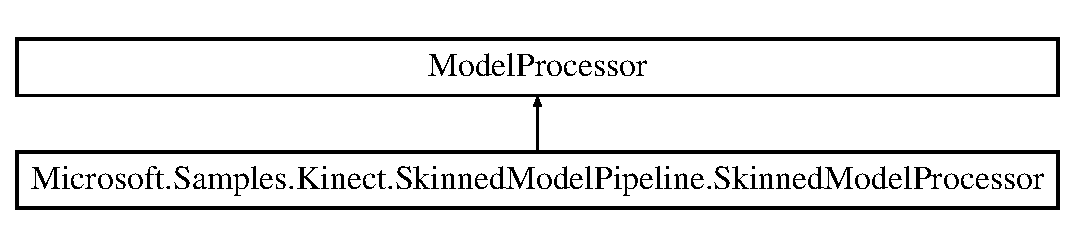
\includegraphics[height=2.000000cm]{class_microsoft_1_1_samples_1_1_kinect_1_1_skinned_model_pipeline_1_1_skinned_model_processor}
\end{center}
\end{figure}
\subsection*{Public Member Functions}
\begin{DoxyCompactItemize}
\item 
override Model\+Content \hyperlink{class_microsoft_1_1_samples_1_1_kinect_1_1_skinned_model_pipeline_1_1_skinned_model_processor_aeb3f8db38e99e916f3cf052e1e588757}{Process} (Node\+Content input, Content\+Processor\+Context context)
\begin{DoxyCompactList}\small\item\em The main Process method converts an intermediate format content pipeline Node\+Content tree to a Model\+Content object with embedded animation data. \end{DoxyCompactList}\end{DoxyCompactItemize}
\subsection*{Static Public Member Functions}
\begin{DoxyCompactItemize}
\item 
static void \hyperlink{class_microsoft_1_1_samples_1_1_kinect_1_1_skinned_model_pipeline_1_1_skinned_model_processor_a15a7a2a1007a8f815f46cd260558b004}{Validate\+Mesh} (Node\+Content node, Content\+Processor\+Context context, string parent\+Bone\+Name)
\begin{DoxyCompactList}\small\item\em Makes sure this mesh contains the kind of data we know how to animate. \end{DoxyCompactList}\item 
static bool \hyperlink{class_microsoft_1_1_samples_1_1_kinect_1_1_skinned_model_pipeline_1_1_skinned_model_processor_a1d13d928dfa3c2ed9a5c9eaa115a0b18}{Mesh\+Has\+Skinning} (Mesh\+Content mesh)
\begin{DoxyCompactList}\small\item\em Checks whether a mesh contains skinning information. \end{DoxyCompactList}\item 
static void \hyperlink{class_microsoft_1_1_samples_1_1_kinect_1_1_skinned_model_pipeline_1_1_skinned_model_processor_a788feaa714f2e3afceb45de2e265b4f5}{Flatten\+Transforms} (Node\+Content node, Bone\+Content skeleton)
\begin{DoxyCompactList}\small\item\em Bakes unwanted transforms into the model geometry, so everything ends up in the same coordinate system. \end{DoxyCompactList}\end{DoxyCompactItemize}
\subsection*{Properties}
\begin{DoxyCompactItemize}
\item 
override \\*
Material\+Processor\+Default\+Effect \hyperlink{class_microsoft_1_1_samples_1_1_kinect_1_1_skinned_model_pipeline_1_1_skinned_model_processor_a15f28361f1525eae7c96ddb05a290a2d}{Default\+Effect}\hspace{0.3cm}{\ttfamily  \mbox{[}get, set\mbox{]}}
\begin{DoxyCompactList}\small\item\em Force all the materials to use our skinned model effect. \end{DoxyCompactList}\end{DoxyCompactItemize}


\subsection{Detailed Description}
Custom processor extends the built in framework Model\+Processor class, adding animation support. 



\subsection{Member Function Documentation}
\hypertarget{class_microsoft_1_1_samples_1_1_kinect_1_1_skinned_model_pipeline_1_1_skinned_model_processor_a788feaa714f2e3afceb45de2e265b4f5}{\index{Microsoft\+::\+Samples\+::\+Kinect\+::\+Skinned\+Model\+Pipeline\+::\+Skinned\+Model\+Processor@{Microsoft\+::\+Samples\+::\+Kinect\+::\+Skinned\+Model\+Pipeline\+::\+Skinned\+Model\+Processor}!Flatten\+Transforms@{Flatten\+Transforms}}
\index{Flatten\+Transforms@{Flatten\+Transforms}!Microsoft\+::\+Samples\+::\+Kinect\+::\+Skinned\+Model\+Pipeline\+::\+Skinned\+Model\+Processor@{Microsoft\+::\+Samples\+::\+Kinect\+::\+Skinned\+Model\+Pipeline\+::\+Skinned\+Model\+Processor}}
\subsubsection[{Flatten\+Transforms}]{\setlength{\rightskip}{0pt plus 5cm}static void Microsoft.\+Samples.\+Kinect.\+Skinned\+Model\+Pipeline.\+Skinned\+Model\+Processor.\+Flatten\+Transforms (
\begin{DoxyParamCaption}
\item[{Node\+Content}]{node, }
\item[{Bone\+Content}]{skeleton}
\end{DoxyParamCaption}
)\hspace{0.3cm}{\ttfamily [static]}}}\label{class_microsoft_1_1_samples_1_1_kinect_1_1_skinned_model_pipeline_1_1_skinned_model_processor_a788feaa714f2e3afceb45de2e265b4f5}


Bakes unwanted transforms into the model geometry, so everything ends up in the same coordinate system. 

\hypertarget{class_microsoft_1_1_samples_1_1_kinect_1_1_skinned_model_pipeline_1_1_skinned_model_processor_a1d13d928dfa3c2ed9a5c9eaa115a0b18}{\index{Microsoft\+::\+Samples\+::\+Kinect\+::\+Skinned\+Model\+Pipeline\+::\+Skinned\+Model\+Processor@{Microsoft\+::\+Samples\+::\+Kinect\+::\+Skinned\+Model\+Pipeline\+::\+Skinned\+Model\+Processor}!Mesh\+Has\+Skinning@{Mesh\+Has\+Skinning}}
\index{Mesh\+Has\+Skinning@{Mesh\+Has\+Skinning}!Microsoft\+::\+Samples\+::\+Kinect\+::\+Skinned\+Model\+Pipeline\+::\+Skinned\+Model\+Processor@{Microsoft\+::\+Samples\+::\+Kinect\+::\+Skinned\+Model\+Pipeline\+::\+Skinned\+Model\+Processor}}
\subsubsection[{Mesh\+Has\+Skinning}]{\setlength{\rightskip}{0pt plus 5cm}static bool Microsoft.\+Samples.\+Kinect.\+Skinned\+Model\+Pipeline.\+Skinned\+Model\+Processor.\+Mesh\+Has\+Skinning (
\begin{DoxyParamCaption}
\item[{Mesh\+Content}]{mesh}
\end{DoxyParamCaption}
)\hspace{0.3cm}{\ttfamily [static]}}}\label{class_microsoft_1_1_samples_1_1_kinect_1_1_skinned_model_pipeline_1_1_skinned_model_processor_a1d13d928dfa3c2ed9a5c9eaa115a0b18}


Checks whether a mesh contains skinning information. 

\begin{DoxyReturn}{Returns}
Returns true if mesh has skin
\end{DoxyReturn}
\hypertarget{class_microsoft_1_1_samples_1_1_kinect_1_1_skinned_model_pipeline_1_1_skinned_model_processor_aeb3f8db38e99e916f3cf052e1e588757}{\index{Microsoft\+::\+Samples\+::\+Kinect\+::\+Skinned\+Model\+Pipeline\+::\+Skinned\+Model\+Processor@{Microsoft\+::\+Samples\+::\+Kinect\+::\+Skinned\+Model\+Pipeline\+::\+Skinned\+Model\+Processor}!Process@{Process}}
\index{Process@{Process}!Microsoft\+::\+Samples\+::\+Kinect\+::\+Skinned\+Model\+Pipeline\+::\+Skinned\+Model\+Processor@{Microsoft\+::\+Samples\+::\+Kinect\+::\+Skinned\+Model\+Pipeline\+::\+Skinned\+Model\+Processor}}
\subsubsection[{Process}]{\setlength{\rightskip}{0pt plus 5cm}override Model\+Content Microsoft.\+Samples.\+Kinect.\+Skinned\+Model\+Pipeline.\+Skinned\+Model\+Processor.\+Process (
\begin{DoxyParamCaption}
\item[{Node\+Content}]{input, }
\item[{Content\+Processor\+Context}]{context}
\end{DoxyParamCaption}
)}}\label{class_microsoft_1_1_samples_1_1_kinect_1_1_skinned_model_pipeline_1_1_skinned_model_processor_aeb3f8db38e99e916f3cf052e1e588757}


The main Process method converts an intermediate format content pipeline Node\+Content tree to a Model\+Content object with embedded animation data. 


\begin{DoxyParams}{Parameters}
{\em input} & Node\+Content input\\
\hline
{\em context} & Content\+Processor\+Context input\\
\hline
\end{DoxyParams}
\begin{DoxyReturn}{Returns}
Model Content
\end{DoxyReturn}
\hypertarget{class_microsoft_1_1_samples_1_1_kinect_1_1_skinned_model_pipeline_1_1_skinned_model_processor_a15a7a2a1007a8f815f46cd260558b004}{\index{Microsoft\+::\+Samples\+::\+Kinect\+::\+Skinned\+Model\+Pipeline\+::\+Skinned\+Model\+Processor@{Microsoft\+::\+Samples\+::\+Kinect\+::\+Skinned\+Model\+Pipeline\+::\+Skinned\+Model\+Processor}!Validate\+Mesh@{Validate\+Mesh}}
\index{Validate\+Mesh@{Validate\+Mesh}!Microsoft\+::\+Samples\+::\+Kinect\+::\+Skinned\+Model\+Pipeline\+::\+Skinned\+Model\+Processor@{Microsoft\+::\+Samples\+::\+Kinect\+::\+Skinned\+Model\+Pipeline\+::\+Skinned\+Model\+Processor}}
\subsubsection[{Validate\+Mesh}]{\setlength{\rightskip}{0pt plus 5cm}static void Microsoft.\+Samples.\+Kinect.\+Skinned\+Model\+Pipeline.\+Skinned\+Model\+Processor.\+Validate\+Mesh (
\begin{DoxyParamCaption}
\item[{Node\+Content}]{node, }
\item[{Content\+Processor\+Context}]{context, }
\item[{string}]{parent\+Bone\+Name}
\end{DoxyParamCaption}
)\hspace{0.3cm}{\ttfamily [static]}}}\label{class_microsoft_1_1_samples_1_1_kinect_1_1_skinned_model_pipeline_1_1_skinned_model_processor_a15a7a2a1007a8f815f46cd260558b004}


Makes sure this mesh contains the kind of data we know how to animate. 



\subsection{Property Documentation}
\hypertarget{class_microsoft_1_1_samples_1_1_kinect_1_1_skinned_model_pipeline_1_1_skinned_model_processor_a15f28361f1525eae7c96ddb05a290a2d}{\index{Microsoft\+::\+Samples\+::\+Kinect\+::\+Skinned\+Model\+Pipeline\+::\+Skinned\+Model\+Processor@{Microsoft\+::\+Samples\+::\+Kinect\+::\+Skinned\+Model\+Pipeline\+::\+Skinned\+Model\+Processor}!Default\+Effect@{Default\+Effect}}
\index{Default\+Effect@{Default\+Effect}!Microsoft\+::\+Samples\+::\+Kinect\+::\+Skinned\+Model\+Pipeline\+::\+Skinned\+Model\+Processor@{Microsoft\+::\+Samples\+::\+Kinect\+::\+Skinned\+Model\+Pipeline\+::\+Skinned\+Model\+Processor}}
\subsubsection[{Default\+Effect}]{\setlength{\rightskip}{0pt plus 5cm}override Material\+Processor\+Default\+Effect Microsoft.\+Samples.\+Kinect.\+Skinned\+Model\+Pipeline.\+Skinned\+Model\+Processor.\+Default\+Effect\hspace{0.3cm}{\ttfamily [get]}, {\ttfamily [set]}}}\label{class_microsoft_1_1_samples_1_1_kinect_1_1_skinned_model_pipeline_1_1_skinned_model_processor_a15f28361f1525eae7c96ddb05a290a2d}


Force all the materials to use our skinned model effect. 



The documentation for this class was generated from the following file\+:\begin{DoxyCompactItemize}
\item 
Skinned\+Model\+Pipeline/Skinned\+Model\+Processor.\+cs\end{DoxyCompactItemize}

\hypertarget{class_skinned_model_1_1_skinning_data}{\section{Skinned\+Model.\+Skinning\+Data Class Reference}
\label{class_skinned_model_1_1_skinning_data}\index{Skinned\+Model.\+Skinning\+Data@{Skinned\+Model.\+Skinning\+Data}}
}


Combines all the data needed to render and animate a skinned object. This is typically stored in the Tag property of the Model being animated.  


\subsection*{Public Member Functions}
\begin{DoxyCompactItemize}
\item 
\hyperlink{class_skinned_model_1_1_skinning_data_afec5d3b876e4a1b553d6aa6b0c88aee5}{Skinning\+Data} (List$<$ Matrix $>$ bind\+Pose, List$<$ Matrix $>$ inverse\+Bind\+Pose, List$<$ int $>$ skeleton\+Hierarchy)
\begin{DoxyCompactList}\small\item\em Initializes a new instance of the \hyperlink{class_skinned_model_1_1_skinning_data}{Skinning\+Data} class. \end{DoxyCompactList}\end{DoxyCompactItemize}
\subsection*{Properties}
\begin{DoxyCompactItemize}
\item 
List$<$ Matrix $>$ \hyperlink{class_skinned_model_1_1_skinning_data_a9cc764c802f632777c48cf7d4cec6e3f}{Bind\+Pose}\hspace{0.3cm}{\ttfamily  \mbox{[}get, set\mbox{]}}
\begin{DoxyCompactList}\small\item\em Bind pose matrices for each bone in the skeleton, relative to the parent bone. \end{DoxyCompactList}\item 
List$<$ Matrix $>$ \hyperlink{class_skinned_model_1_1_skinning_data_a480419d9a7614d8e72b95e694d9ce908}{Inverse\+Bind\+Pose}\hspace{0.3cm}{\ttfamily  \mbox{[}get, set\mbox{]}}
\begin{DoxyCompactList}\small\item\em Vertex to bone space transforms for each bone in the skeleton. \end{DoxyCompactList}\item 
List$<$ int $>$ \hyperlink{class_skinned_model_1_1_skinning_data_a83e303f9faee1c4c121897106a450f30}{Skeleton\+Hierarchy}\hspace{0.3cm}{\ttfamily  \mbox{[}get, set\mbox{]}}
\begin{DoxyCompactList}\small\item\em For each bone in the skeleton, stores the index of the parent bone. \end{DoxyCompactList}\end{DoxyCompactItemize}


\subsection{Detailed Description}
Combines all the data needed to render and animate a skinned object. This is typically stored in the Tag property of the Model being animated. 



\subsection{Constructor \& Destructor Documentation}
\hypertarget{class_skinned_model_1_1_skinning_data_afec5d3b876e4a1b553d6aa6b0c88aee5}{\index{Skinned\+Model\+::\+Skinning\+Data@{Skinned\+Model\+::\+Skinning\+Data}!Skinning\+Data@{Skinning\+Data}}
\index{Skinning\+Data@{Skinning\+Data}!Skinned\+Model\+::\+Skinning\+Data@{Skinned\+Model\+::\+Skinning\+Data}}
\subsubsection[{Skinning\+Data}]{\setlength{\rightskip}{0pt plus 5cm}Skinned\+Model.\+Skinning\+Data.\+Skinning\+Data (
\begin{DoxyParamCaption}
\item[{List$<$ Matrix $>$}]{bind\+Pose, }
\item[{List$<$ Matrix $>$}]{inverse\+Bind\+Pose, }
\item[{List$<$ int $>$}]{skeleton\+Hierarchy}
\end{DoxyParamCaption}
)}}\label{class_skinned_model_1_1_skinning_data_afec5d3b876e4a1b553d6aa6b0c88aee5}


Initializes a new instance of the \hyperlink{class_skinned_model_1_1_skinning_data}{Skinning\+Data} class. 



\subsection{Property Documentation}
\hypertarget{class_skinned_model_1_1_skinning_data_a9cc764c802f632777c48cf7d4cec6e3f}{\index{Skinned\+Model\+::\+Skinning\+Data@{Skinned\+Model\+::\+Skinning\+Data}!Bind\+Pose@{Bind\+Pose}}
\index{Bind\+Pose@{Bind\+Pose}!Skinned\+Model\+::\+Skinning\+Data@{Skinned\+Model\+::\+Skinning\+Data}}
\subsubsection[{Bind\+Pose}]{\setlength{\rightskip}{0pt plus 5cm}List$<$Matrix$>$ Skinned\+Model.\+Skinning\+Data.\+Bind\+Pose\hspace{0.3cm}{\ttfamily [get]}, {\ttfamily [set]}}}\label{class_skinned_model_1_1_skinning_data_a9cc764c802f632777c48cf7d4cec6e3f}


Bind pose matrices for each bone in the skeleton, relative to the parent bone. 

\hypertarget{class_skinned_model_1_1_skinning_data_a480419d9a7614d8e72b95e694d9ce908}{\index{Skinned\+Model\+::\+Skinning\+Data@{Skinned\+Model\+::\+Skinning\+Data}!Inverse\+Bind\+Pose@{Inverse\+Bind\+Pose}}
\index{Inverse\+Bind\+Pose@{Inverse\+Bind\+Pose}!Skinned\+Model\+::\+Skinning\+Data@{Skinned\+Model\+::\+Skinning\+Data}}
\subsubsection[{Inverse\+Bind\+Pose}]{\setlength{\rightskip}{0pt plus 5cm}List$<$Matrix$>$ Skinned\+Model.\+Skinning\+Data.\+Inverse\+Bind\+Pose\hspace{0.3cm}{\ttfamily [get]}, {\ttfamily [set]}}}\label{class_skinned_model_1_1_skinning_data_a480419d9a7614d8e72b95e694d9ce908}


Vertex to bone space transforms for each bone in the skeleton. 

\hypertarget{class_skinned_model_1_1_skinning_data_a83e303f9faee1c4c121897106a450f30}{\index{Skinned\+Model\+::\+Skinning\+Data@{Skinned\+Model\+::\+Skinning\+Data}!Skeleton\+Hierarchy@{Skeleton\+Hierarchy}}
\index{Skeleton\+Hierarchy@{Skeleton\+Hierarchy}!Skinned\+Model\+::\+Skinning\+Data@{Skinned\+Model\+::\+Skinning\+Data}}
\subsubsection[{Skeleton\+Hierarchy}]{\setlength{\rightskip}{0pt plus 5cm}List$<$int$>$ Skinned\+Model.\+Skinning\+Data.\+Skeleton\+Hierarchy\hspace{0.3cm}{\ttfamily [get]}, {\ttfamily [set]}}}\label{class_skinned_model_1_1_skinning_data_a83e303f9faee1c4c121897106a450f30}


For each bone in the skeleton, stores the index of the parent bone. 



The documentation for this class was generated from the following file\+:\begin{DoxyCompactItemize}
\item 
Skinned\+Model/Skinning\+Data.\+cs\end{DoxyCompactItemize}

\hypertarget{class_microsoft_1_1_samples_1_1_kinect_1_1_avateering_1_1_filters_1_1_timed_lerp}{\section{Microsoft.\+Samples.\+Kinect.\+Avateering.\+Filters.\+Timed\+Lerp Class Reference}
\label{class_microsoft_1_1_samples_1_1_kinect_1_1_avateering_1_1_filters_1_1_timed_lerp}\index{Microsoft.\+Samples.\+Kinect.\+Avateering.\+Filters.\+Timed\+Lerp@{Microsoft.\+Samples.\+Kinect.\+Avateering.\+Filters.\+Timed\+Lerp}}
}


\hyperlink{class_microsoft_1_1_samples_1_1_kinect_1_1_avateering_1_1_filters_1_1_timed_lerp}{Timed\+Lerp} -\/ Maintains a time-\/based lerp between 0 and a upper limit between 0 and 1. The lerp speed parameter is in units of inverse time -\/ therefore, a speed of 2.\+0 means that the lerp completes a full transition (0 to 1) in 0.\+5 seconds.  


\subsection*{Public Member Functions}
\begin{DoxyCompactItemize}
\item 
\hyperlink{class_microsoft_1_1_samples_1_1_kinect_1_1_avateering_1_1_filters_1_1_timed_lerp_a2fb853bc9258623a8661f0ce980d8482}{Timed\+Lerp} ()
\begin{DoxyCompactList}\small\item\em Initializes a new instance of the \hyperlink{class_microsoft_1_1_samples_1_1_kinect_1_1_avateering_1_1_filters_1_1_timed_lerp}{Timed\+Lerp} class. \end{DoxyCompactList}\item 
void \hyperlink{class_microsoft_1_1_samples_1_1_kinect_1_1_avateering_1_1_filters_1_1_timed_lerp_a7b000562840aed3cb22da5305887c75f}{Set\+Speed} ()
\begin{DoxyCompactList}\small\item\em Set speeds. \end{DoxyCompactList}\item 
void \hyperlink{class_microsoft_1_1_samples_1_1_kinect_1_1_avateering_1_1_filters_1_1_timed_lerp_a8c7da8003befabf88f27664f620edcc1}{Set\+Speed} (float ease\+In\+Speed, float ease\+Out\+Speed)
\begin{DoxyCompactList}\small\item\em Set speeds. \end{DoxyCompactList}\item 
void \hyperlink{class_microsoft_1_1_samples_1_1_kinect_1_1_avateering_1_1_filters_1_1_timed_lerp_a9528c6e4965ee4613ee2078369cea2e7}{Set\+Enabled} (bool is\+Enabled)
\begin{DoxyCompactList}\small\item\em Set whether the Lerp is enabled. \end{DoxyCompactList}\item 
void \hyperlink{class_microsoft_1_1_samples_1_1_kinect_1_1_avateering_1_1_filters_1_1_timed_lerp_a4f6ccd18411293b7713d22fed18c6cef}{Set\+Enabled} (float enabled)
\begin{DoxyCompactList}\small\item\em Set the Lerp enable value. \end{DoxyCompactList}\item 
void \hyperlink{class_microsoft_1_1_samples_1_1_kinect_1_1_avateering_1_1_filters_1_1_timed_lerp_a66bc729b694f75f320315d7fe374d4c8}{Reset} ()
\begin{DoxyCompactList}\small\item\em Re\+Set the Lerp. \end{DoxyCompactList}\item 
bool \hyperlink{class_microsoft_1_1_samples_1_1_kinect_1_1_avateering_1_1_filters_1_1_timed_lerp_ab8f4dca739b0f1240a1bde6fa949fcdb}{Is\+Enabled} ()
\begin{DoxyCompactList}\small\item\em Is\+Enabled reflects whether the target value is 0 or not. \end{DoxyCompactList}\item 
bool \hyperlink{class_microsoft_1_1_samples_1_1_kinect_1_1_avateering_1_1_filters_1_1_timed_lerp_afbd26c2a019f4208b1b4fde7c0795a3a}{Is\+Lerp\+Enabled} ()
\begin{DoxyCompactList}\small\item\em Is\+Lerp\+Enabled reflects whether the current value is 0 or not. \end{DoxyCompactList}\item 
void \hyperlink{class_microsoft_1_1_samples_1_1_kinect_1_1_avateering_1_1_filters_1_1_timed_lerp_a253aa6f84dbfc579ba0e89a97bdfb537}{Tick} (float delta\+Time)
\begin{DoxyCompactList}\small\item\em Tick needs to be called once per frame. \end{DoxyCompactList}\end{DoxyCompactItemize}
\subsection*{Properties}
\begin{DoxyCompactItemize}
\item 
float \hyperlink{class_microsoft_1_1_samples_1_1_kinect_1_1_avateering_1_1_filters_1_1_timed_lerp_a3b40018bedff53d1fcbb9846819546a9}{Linear\+Value}\hspace{0.3cm}{\ttfamily  \mbox{[}get\mbox{]}}
\begin{DoxyCompactList}\small\item\em Gets Linear\+Value. Returns a raw, linearly interpolated value between 0 and the Math.\+Maximum value. \end{DoxyCompactList}\item 
float \hyperlink{class_microsoft_1_1_samples_1_1_kinect_1_1_avateering_1_1_filters_1_1_timed_lerp_a6dcdd78c7c307469b295ae76b5b41eda}{Smooth\+Value}\hspace{0.3cm}{\ttfamily  \mbox{[}get\mbox{]}}
\begin{DoxyCompactList}\small\item\em Gets Smooth\+Value. Returns the value between 0 and the Math.\+Maximum value, but applies a cosine-\/shaped smoothing function. \end{DoxyCompactList}\item 
float \hyperlink{class_microsoft_1_1_samples_1_1_kinect_1_1_avateering_1_1_filters_1_1_timed_lerp_ab64a8022d62f23eae5f19239dd734b1a}{Enabled}\hspace{0.3cm}{\ttfamily  \mbox{[}get, set\mbox{]}}
\begin{DoxyCompactList}\small\item\em Gets or sets Enabled value. \end{DoxyCompactList}\item 
float \hyperlink{class_microsoft_1_1_samples_1_1_kinect_1_1_avateering_1_1_filters_1_1_timed_lerp_a5f0d73e5e719721431fe9aa90b863788}{Value}\hspace{0.3cm}{\ttfamily  \mbox{[}get, set\mbox{]}}
\begin{DoxyCompactList}\small\item\em Gets or sets The Value. \end{DoxyCompactList}\item 
float \hyperlink{class_microsoft_1_1_samples_1_1_kinect_1_1_avateering_1_1_filters_1_1_timed_lerp_ae01477cadfec29642886ebc8f61c9a1c}{Ease\+In\+Speed}\hspace{0.3cm}{\ttfamily  \mbox{[}get, set\mbox{]}}
\begin{DoxyCompactList}\small\item\em Gets or sets Ease in speed. \end{DoxyCompactList}\item 
float \hyperlink{class_microsoft_1_1_samples_1_1_kinect_1_1_avateering_1_1_filters_1_1_timed_lerp_a623a5eb25a0d10237079b75be47b394e}{Ease\+Out\+Speed}\hspace{0.3cm}{\ttfamily  \mbox{[}get, set\mbox{]}}
\begin{DoxyCompactList}\small\item\em Gets or sets Ease out speed. \end{DoxyCompactList}\end{DoxyCompactItemize}


\subsection{Detailed Description}
\hyperlink{class_microsoft_1_1_samples_1_1_kinect_1_1_avateering_1_1_filters_1_1_timed_lerp}{Timed\+Lerp} -\/ Maintains a time-\/based lerp between 0 and a upper limit between 0 and 1. The lerp speed parameter is in units of inverse time -\/ therefore, a speed of 2.\+0 means that the lerp completes a full transition (0 to 1) in 0.\+5 seconds. 



\subsection{Constructor \& Destructor Documentation}
\hypertarget{class_microsoft_1_1_samples_1_1_kinect_1_1_avateering_1_1_filters_1_1_timed_lerp_a2fb853bc9258623a8661f0ce980d8482}{\index{Microsoft\+::\+Samples\+::\+Kinect\+::\+Avateering\+::\+Filters\+::\+Timed\+Lerp@{Microsoft\+::\+Samples\+::\+Kinect\+::\+Avateering\+::\+Filters\+::\+Timed\+Lerp}!Timed\+Lerp@{Timed\+Lerp}}
\index{Timed\+Lerp@{Timed\+Lerp}!Microsoft\+::\+Samples\+::\+Kinect\+::\+Avateering\+::\+Filters\+::\+Timed\+Lerp@{Microsoft\+::\+Samples\+::\+Kinect\+::\+Avateering\+::\+Filters\+::\+Timed\+Lerp}}
\subsubsection[{Timed\+Lerp}]{\setlength{\rightskip}{0pt plus 5cm}Microsoft.\+Samples.\+Kinect.\+Avateering.\+Filters.\+Timed\+Lerp.\+Timed\+Lerp (
\begin{DoxyParamCaption}
{}
\end{DoxyParamCaption}
)}}\label{class_microsoft_1_1_samples_1_1_kinect_1_1_avateering_1_1_filters_1_1_timed_lerp_a2fb853bc9258623a8661f0ce980d8482}


Initializes a new instance of the \hyperlink{class_microsoft_1_1_samples_1_1_kinect_1_1_avateering_1_1_filters_1_1_timed_lerp}{Timed\+Lerp} class. 



\subsection{Member Function Documentation}
\hypertarget{class_microsoft_1_1_samples_1_1_kinect_1_1_avateering_1_1_filters_1_1_timed_lerp_ab8f4dca739b0f1240a1bde6fa949fcdb}{\index{Microsoft\+::\+Samples\+::\+Kinect\+::\+Avateering\+::\+Filters\+::\+Timed\+Lerp@{Microsoft\+::\+Samples\+::\+Kinect\+::\+Avateering\+::\+Filters\+::\+Timed\+Lerp}!Is\+Enabled@{Is\+Enabled}}
\index{Is\+Enabled@{Is\+Enabled}!Microsoft\+::\+Samples\+::\+Kinect\+::\+Avateering\+::\+Filters\+::\+Timed\+Lerp@{Microsoft\+::\+Samples\+::\+Kinect\+::\+Avateering\+::\+Filters\+::\+Timed\+Lerp}}
\subsubsection[{Is\+Enabled}]{\setlength{\rightskip}{0pt plus 5cm}bool Microsoft.\+Samples.\+Kinect.\+Avateering.\+Filters.\+Timed\+Lerp.\+Is\+Enabled (
\begin{DoxyParamCaption}
{}
\end{DoxyParamCaption}
)}}\label{class_microsoft_1_1_samples_1_1_kinect_1_1_avateering_1_1_filters_1_1_timed_lerp_ab8f4dca739b0f1240a1bde6fa949fcdb}


Is\+Enabled reflects whether the target value is 0 or not. 

\begin{DoxyReturn}{Returns}
Returns true if enabled.
\end{DoxyReturn}
\hypertarget{class_microsoft_1_1_samples_1_1_kinect_1_1_avateering_1_1_filters_1_1_timed_lerp_afbd26c2a019f4208b1b4fde7c0795a3a}{\index{Microsoft\+::\+Samples\+::\+Kinect\+::\+Avateering\+::\+Filters\+::\+Timed\+Lerp@{Microsoft\+::\+Samples\+::\+Kinect\+::\+Avateering\+::\+Filters\+::\+Timed\+Lerp}!Is\+Lerp\+Enabled@{Is\+Lerp\+Enabled}}
\index{Is\+Lerp\+Enabled@{Is\+Lerp\+Enabled}!Microsoft\+::\+Samples\+::\+Kinect\+::\+Avateering\+::\+Filters\+::\+Timed\+Lerp@{Microsoft\+::\+Samples\+::\+Kinect\+::\+Avateering\+::\+Filters\+::\+Timed\+Lerp}}
\subsubsection[{Is\+Lerp\+Enabled}]{\setlength{\rightskip}{0pt plus 5cm}bool Microsoft.\+Samples.\+Kinect.\+Avateering.\+Filters.\+Timed\+Lerp.\+Is\+Lerp\+Enabled (
\begin{DoxyParamCaption}
{}
\end{DoxyParamCaption}
)}}\label{class_microsoft_1_1_samples_1_1_kinect_1_1_avateering_1_1_filters_1_1_timed_lerp_afbd26c2a019f4208b1b4fde7c0795a3a}


Is\+Lerp\+Enabled reflects whether the current value is 0 or not. 

\begin{DoxyReturn}{Returns}
Returns true if enabled and value greater than 0, false otherwise.
\end{DoxyReturn}
\hypertarget{class_microsoft_1_1_samples_1_1_kinect_1_1_avateering_1_1_filters_1_1_timed_lerp_a66bc729b694f75f320315d7fe374d4c8}{\index{Microsoft\+::\+Samples\+::\+Kinect\+::\+Avateering\+::\+Filters\+::\+Timed\+Lerp@{Microsoft\+::\+Samples\+::\+Kinect\+::\+Avateering\+::\+Filters\+::\+Timed\+Lerp}!Reset@{Reset}}
\index{Reset@{Reset}!Microsoft\+::\+Samples\+::\+Kinect\+::\+Avateering\+::\+Filters\+::\+Timed\+Lerp@{Microsoft\+::\+Samples\+::\+Kinect\+::\+Avateering\+::\+Filters\+::\+Timed\+Lerp}}
\subsubsection[{Reset}]{\setlength{\rightskip}{0pt plus 5cm}void Microsoft.\+Samples.\+Kinect.\+Avateering.\+Filters.\+Timed\+Lerp.\+Reset (
\begin{DoxyParamCaption}
{}
\end{DoxyParamCaption}
)}}\label{class_microsoft_1_1_samples_1_1_kinect_1_1_avateering_1_1_filters_1_1_timed_lerp_a66bc729b694f75f320315d7fe374d4c8}


Re\+Set the Lerp. 

\hypertarget{class_microsoft_1_1_samples_1_1_kinect_1_1_avateering_1_1_filters_1_1_timed_lerp_a9528c6e4965ee4613ee2078369cea2e7}{\index{Microsoft\+::\+Samples\+::\+Kinect\+::\+Avateering\+::\+Filters\+::\+Timed\+Lerp@{Microsoft\+::\+Samples\+::\+Kinect\+::\+Avateering\+::\+Filters\+::\+Timed\+Lerp}!Set\+Enabled@{Set\+Enabled}}
\index{Set\+Enabled@{Set\+Enabled}!Microsoft\+::\+Samples\+::\+Kinect\+::\+Avateering\+::\+Filters\+::\+Timed\+Lerp@{Microsoft\+::\+Samples\+::\+Kinect\+::\+Avateering\+::\+Filters\+::\+Timed\+Lerp}}
\subsubsection[{Set\+Enabled}]{\setlength{\rightskip}{0pt plus 5cm}void Microsoft.\+Samples.\+Kinect.\+Avateering.\+Filters.\+Timed\+Lerp.\+Set\+Enabled (
\begin{DoxyParamCaption}
\item[{bool}]{is\+Enabled}
\end{DoxyParamCaption}
)}}\label{class_microsoft_1_1_samples_1_1_kinect_1_1_avateering_1_1_filters_1_1_timed_lerp_a9528c6e4965ee4613ee2078369cea2e7}


Set whether the Lerp is enabled. 


\begin{DoxyParams}{Parameters}
{\em is\+Enabled} & Enable or Disable Lerp.\\
\hline
\end{DoxyParams}
\hypertarget{class_microsoft_1_1_samples_1_1_kinect_1_1_avateering_1_1_filters_1_1_timed_lerp_a4f6ccd18411293b7713d22fed18c6cef}{\index{Microsoft\+::\+Samples\+::\+Kinect\+::\+Avateering\+::\+Filters\+::\+Timed\+Lerp@{Microsoft\+::\+Samples\+::\+Kinect\+::\+Avateering\+::\+Filters\+::\+Timed\+Lerp}!Set\+Enabled@{Set\+Enabled}}
\index{Set\+Enabled@{Set\+Enabled}!Microsoft\+::\+Samples\+::\+Kinect\+::\+Avateering\+::\+Filters\+::\+Timed\+Lerp@{Microsoft\+::\+Samples\+::\+Kinect\+::\+Avateering\+::\+Filters\+::\+Timed\+Lerp}}
\subsubsection[{Set\+Enabled}]{\setlength{\rightskip}{0pt plus 5cm}void Microsoft.\+Samples.\+Kinect.\+Avateering.\+Filters.\+Timed\+Lerp.\+Set\+Enabled (
\begin{DoxyParamCaption}
\item[{float}]{enabled}
\end{DoxyParamCaption}
)}}\label{class_microsoft_1_1_samples_1_1_kinect_1_1_avateering_1_1_filters_1_1_timed_lerp_a4f6ccd18411293b7713d22fed18c6cef}


Set the Lerp enable value. 


\begin{DoxyParams}{Parameters}
{\em enabled} & Set enable value.\\
\hline
\end{DoxyParams}
\hypertarget{class_microsoft_1_1_samples_1_1_kinect_1_1_avateering_1_1_filters_1_1_timed_lerp_a7b000562840aed3cb22da5305887c75f}{\index{Microsoft\+::\+Samples\+::\+Kinect\+::\+Avateering\+::\+Filters\+::\+Timed\+Lerp@{Microsoft\+::\+Samples\+::\+Kinect\+::\+Avateering\+::\+Filters\+::\+Timed\+Lerp}!Set\+Speed@{Set\+Speed}}
\index{Set\+Speed@{Set\+Speed}!Microsoft\+::\+Samples\+::\+Kinect\+::\+Avateering\+::\+Filters\+::\+Timed\+Lerp@{Microsoft\+::\+Samples\+::\+Kinect\+::\+Avateering\+::\+Filters\+::\+Timed\+Lerp}}
\subsubsection[{Set\+Speed}]{\setlength{\rightskip}{0pt plus 5cm}void Microsoft.\+Samples.\+Kinect.\+Avateering.\+Filters.\+Timed\+Lerp.\+Set\+Speed (
\begin{DoxyParamCaption}
{}
\end{DoxyParamCaption}
)}}\label{class_microsoft_1_1_samples_1_1_kinect_1_1_avateering_1_1_filters_1_1_timed_lerp_a7b000562840aed3cb22da5305887c75f}


Set speeds. 

\hypertarget{class_microsoft_1_1_samples_1_1_kinect_1_1_avateering_1_1_filters_1_1_timed_lerp_a8c7da8003befabf88f27664f620edcc1}{\index{Microsoft\+::\+Samples\+::\+Kinect\+::\+Avateering\+::\+Filters\+::\+Timed\+Lerp@{Microsoft\+::\+Samples\+::\+Kinect\+::\+Avateering\+::\+Filters\+::\+Timed\+Lerp}!Set\+Speed@{Set\+Speed}}
\index{Set\+Speed@{Set\+Speed}!Microsoft\+::\+Samples\+::\+Kinect\+::\+Avateering\+::\+Filters\+::\+Timed\+Lerp@{Microsoft\+::\+Samples\+::\+Kinect\+::\+Avateering\+::\+Filters\+::\+Timed\+Lerp}}
\subsubsection[{Set\+Speed}]{\setlength{\rightskip}{0pt plus 5cm}void Microsoft.\+Samples.\+Kinect.\+Avateering.\+Filters.\+Timed\+Lerp.\+Set\+Speed (
\begin{DoxyParamCaption}
\item[{float}]{ease\+In\+Speed, }
\item[{float}]{ease\+Out\+Speed}
\end{DoxyParamCaption}
)}}\label{class_microsoft_1_1_samples_1_1_kinect_1_1_avateering_1_1_filters_1_1_timed_lerp_a8c7da8003befabf88f27664f620edcc1}


Set speeds. 


\begin{DoxyParams}{Parameters}
{\em ease\+In\+Speed} & Ease in speed value.\\
\hline
{\em ease\+Out\+Speed} & Ease out speed value.\\
\hline
\end{DoxyParams}
\hypertarget{class_microsoft_1_1_samples_1_1_kinect_1_1_avateering_1_1_filters_1_1_timed_lerp_a253aa6f84dbfc579ba0e89a97bdfb537}{\index{Microsoft\+::\+Samples\+::\+Kinect\+::\+Avateering\+::\+Filters\+::\+Timed\+Lerp@{Microsoft\+::\+Samples\+::\+Kinect\+::\+Avateering\+::\+Filters\+::\+Timed\+Lerp}!Tick@{Tick}}
\index{Tick@{Tick}!Microsoft\+::\+Samples\+::\+Kinect\+::\+Avateering\+::\+Filters\+::\+Timed\+Lerp@{Microsoft\+::\+Samples\+::\+Kinect\+::\+Avateering\+::\+Filters\+::\+Timed\+Lerp}}
\subsubsection[{Tick}]{\setlength{\rightskip}{0pt plus 5cm}void Microsoft.\+Samples.\+Kinect.\+Avateering.\+Filters.\+Timed\+Lerp.\+Tick (
\begin{DoxyParamCaption}
\item[{float}]{delta\+Time}
\end{DoxyParamCaption}
)}}\label{class_microsoft_1_1_samples_1_1_kinect_1_1_avateering_1_1_filters_1_1_timed_lerp_a253aa6f84dbfc579ba0e89a97bdfb537}


Tick needs to be called once per frame. 


\begin{DoxyParams}{Parameters}
{\em delta\+Time} & The time difference between frames.\\
\hline
\end{DoxyParams}


\subsection{Property Documentation}
\hypertarget{class_microsoft_1_1_samples_1_1_kinect_1_1_avateering_1_1_filters_1_1_timed_lerp_ae01477cadfec29642886ebc8f61c9a1c}{\index{Microsoft\+::\+Samples\+::\+Kinect\+::\+Avateering\+::\+Filters\+::\+Timed\+Lerp@{Microsoft\+::\+Samples\+::\+Kinect\+::\+Avateering\+::\+Filters\+::\+Timed\+Lerp}!Ease\+In\+Speed@{Ease\+In\+Speed}}
\index{Ease\+In\+Speed@{Ease\+In\+Speed}!Microsoft\+::\+Samples\+::\+Kinect\+::\+Avateering\+::\+Filters\+::\+Timed\+Lerp@{Microsoft\+::\+Samples\+::\+Kinect\+::\+Avateering\+::\+Filters\+::\+Timed\+Lerp}}
\subsubsection[{Ease\+In\+Speed}]{\setlength{\rightskip}{0pt plus 5cm}float Microsoft.\+Samples.\+Kinect.\+Avateering.\+Filters.\+Timed\+Lerp.\+Ease\+In\+Speed\hspace{0.3cm}{\ttfamily [get]}, {\ttfamily [set]}, {\ttfamily [protected]}}}\label{class_microsoft_1_1_samples_1_1_kinect_1_1_avateering_1_1_filters_1_1_timed_lerp_ae01477cadfec29642886ebc8f61c9a1c}


Gets or sets Ease in speed. 

\hypertarget{class_microsoft_1_1_samples_1_1_kinect_1_1_avateering_1_1_filters_1_1_timed_lerp_a623a5eb25a0d10237079b75be47b394e}{\index{Microsoft\+::\+Samples\+::\+Kinect\+::\+Avateering\+::\+Filters\+::\+Timed\+Lerp@{Microsoft\+::\+Samples\+::\+Kinect\+::\+Avateering\+::\+Filters\+::\+Timed\+Lerp}!Ease\+Out\+Speed@{Ease\+Out\+Speed}}
\index{Ease\+Out\+Speed@{Ease\+Out\+Speed}!Microsoft\+::\+Samples\+::\+Kinect\+::\+Avateering\+::\+Filters\+::\+Timed\+Lerp@{Microsoft\+::\+Samples\+::\+Kinect\+::\+Avateering\+::\+Filters\+::\+Timed\+Lerp}}
\subsubsection[{Ease\+Out\+Speed}]{\setlength{\rightskip}{0pt plus 5cm}float Microsoft.\+Samples.\+Kinect.\+Avateering.\+Filters.\+Timed\+Lerp.\+Ease\+Out\+Speed\hspace{0.3cm}{\ttfamily [get]}, {\ttfamily [set]}, {\ttfamily [protected]}}}\label{class_microsoft_1_1_samples_1_1_kinect_1_1_avateering_1_1_filters_1_1_timed_lerp_a623a5eb25a0d10237079b75be47b394e}


Gets or sets Ease out speed. 

\hypertarget{class_microsoft_1_1_samples_1_1_kinect_1_1_avateering_1_1_filters_1_1_timed_lerp_ab64a8022d62f23eae5f19239dd734b1a}{\index{Microsoft\+::\+Samples\+::\+Kinect\+::\+Avateering\+::\+Filters\+::\+Timed\+Lerp@{Microsoft\+::\+Samples\+::\+Kinect\+::\+Avateering\+::\+Filters\+::\+Timed\+Lerp}!Enabled@{Enabled}}
\index{Enabled@{Enabled}!Microsoft\+::\+Samples\+::\+Kinect\+::\+Avateering\+::\+Filters\+::\+Timed\+Lerp@{Microsoft\+::\+Samples\+::\+Kinect\+::\+Avateering\+::\+Filters\+::\+Timed\+Lerp}}
\subsubsection[{Enabled}]{\setlength{\rightskip}{0pt plus 5cm}float Microsoft.\+Samples.\+Kinect.\+Avateering.\+Filters.\+Timed\+Lerp.\+Enabled\hspace{0.3cm}{\ttfamily [get]}, {\ttfamily [set]}, {\ttfamily [protected]}}}\label{class_microsoft_1_1_samples_1_1_kinect_1_1_avateering_1_1_filters_1_1_timed_lerp_ab64a8022d62f23eae5f19239dd734b1a}


Gets or sets Enabled value. 

\hypertarget{class_microsoft_1_1_samples_1_1_kinect_1_1_avateering_1_1_filters_1_1_timed_lerp_a3b40018bedff53d1fcbb9846819546a9}{\index{Microsoft\+::\+Samples\+::\+Kinect\+::\+Avateering\+::\+Filters\+::\+Timed\+Lerp@{Microsoft\+::\+Samples\+::\+Kinect\+::\+Avateering\+::\+Filters\+::\+Timed\+Lerp}!Linear\+Value@{Linear\+Value}}
\index{Linear\+Value@{Linear\+Value}!Microsoft\+::\+Samples\+::\+Kinect\+::\+Avateering\+::\+Filters\+::\+Timed\+Lerp@{Microsoft\+::\+Samples\+::\+Kinect\+::\+Avateering\+::\+Filters\+::\+Timed\+Lerp}}
\subsubsection[{Linear\+Value}]{\setlength{\rightskip}{0pt plus 5cm}float Microsoft.\+Samples.\+Kinect.\+Avateering.\+Filters.\+Timed\+Lerp.\+Linear\+Value\hspace{0.3cm}{\ttfamily [get]}}}\label{class_microsoft_1_1_samples_1_1_kinect_1_1_avateering_1_1_filters_1_1_timed_lerp_a3b40018bedff53d1fcbb9846819546a9}


Gets Linear\+Value. Returns a raw, linearly interpolated value between 0 and the Math.\+Maximum value. 

\begin{DoxyReturn}{Returns}
Returns a linear Lerped value.
\end{DoxyReturn}
\hypertarget{class_microsoft_1_1_samples_1_1_kinect_1_1_avateering_1_1_filters_1_1_timed_lerp_a6dcdd78c7c307469b295ae76b5b41eda}{\index{Microsoft\+::\+Samples\+::\+Kinect\+::\+Avateering\+::\+Filters\+::\+Timed\+Lerp@{Microsoft\+::\+Samples\+::\+Kinect\+::\+Avateering\+::\+Filters\+::\+Timed\+Lerp}!Smooth\+Value@{Smooth\+Value}}
\index{Smooth\+Value@{Smooth\+Value}!Microsoft\+::\+Samples\+::\+Kinect\+::\+Avateering\+::\+Filters\+::\+Timed\+Lerp@{Microsoft\+::\+Samples\+::\+Kinect\+::\+Avateering\+::\+Filters\+::\+Timed\+Lerp}}
\subsubsection[{Smooth\+Value}]{\setlength{\rightskip}{0pt plus 5cm}float Microsoft.\+Samples.\+Kinect.\+Avateering.\+Filters.\+Timed\+Lerp.\+Smooth\+Value\hspace{0.3cm}{\ttfamily [get]}}}\label{class_microsoft_1_1_samples_1_1_kinect_1_1_avateering_1_1_filters_1_1_timed_lerp_a6dcdd78c7c307469b295ae76b5b41eda}


Gets Smooth\+Value. Returns the value between 0 and the Math.\+Maximum value, but applies a cosine-\/shaped smoothing function. 

\begin{DoxyReturn}{Returns}
Returns a smoothed value.
\end{DoxyReturn}
\hypertarget{class_microsoft_1_1_samples_1_1_kinect_1_1_avateering_1_1_filters_1_1_timed_lerp_a5f0d73e5e719721431fe9aa90b863788}{\index{Microsoft\+::\+Samples\+::\+Kinect\+::\+Avateering\+::\+Filters\+::\+Timed\+Lerp@{Microsoft\+::\+Samples\+::\+Kinect\+::\+Avateering\+::\+Filters\+::\+Timed\+Lerp}!Value@{Value}}
\index{Value@{Value}!Microsoft\+::\+Samples\+::\+Kinect\+::\+Avateering\+::\+Filters\+::\+Timed\+Lerp@{Microsoft\+::\+Samples\+::\+Kinect\+::\+Avateering\+::\+Filters\+::\+Timed\+Lerp}}
\subsubsection[{Value}]{\setlength{\rightskip}{0pt plus 5cm}float Microsoft.\+Samples.\+Kinect.\+Avateering.\+Filters.\+Timed\+Lerp.\+Value\hspace{0.3cm}{\ttfamily [get]}, {\ttfamily [set]}, {\ttfamily [protected]}}}\label{class_microsoft_1_1_samples_1_1_kinect_1_1_avateering_1_1_filters_1_1_timed_lerp_a5f0d73e5e719721431fe9aa90b863788}


Gets or sets The Value. 



The documentation for this class was generated from the following file\+:\begin{DoxyCompactItemize}
\item 
Avateering/\+Filters/Timed\+Lerp.\+cs\end{DoxyCompactItemize}

\hypertarget{class_microsoft_1_1_samples_1_1_kinect_1_1_avateering_1_1_filters_1_1_timer}{\section{Microsoft.\+Samples.\+Kinect.\+Avateering.\+Filters.\+Timer Class Reference}
\label{class_microsoft_1_1_samples_1_1_kinect_1_1_avateering_1_1_filters_1_1_timer}\index{Microsoft.\+Samples.\+Kinect.\+Avateering.\+Filters.\+Timer@{Microsoft.\+Samples.\+Kinect.\+Avateering.\+Filters.\+Timer}}
}


Class \hyperlink{class_microsoft_1_1_samples_1_1_kinect_1_1_avateering_1_1_filters_1_1_timer}{Timer} is a helper class to perform timer operations For stop-\/watch timer functionality, use\+: \hyperlink{class_microsoft_1_1_samples_1_1_kinect_1_1_avateering_1_1_filters_1_1_timer_a463741040cda49273475a5722322b73d}{Start()} -\/ To start the timer \hyperlink{class_microsoft_1_1_samples_1_1_kinect_1_1_avateering_1_1_filters_1_1_timer_a018da7ed7832a2257569dd87e68e6137}{Stop()} -\/ To stop (or pause) the timer \hyperlink{class_microsoft_1_1_samples_1_1_kinect_1_1_avateering_1_1_filters_1_1_timer_a938e1304e5e4aaa916a5ef010ff8fc28}{Reset()} -\/ To reset the timer Time -\/ Returns current time or last stopped time For app-\/timing and per-\/frame updates, use\+: Absolute\+Time -\/ To get the absolute system time Get\+App\+Time() -\/ To get the running time since construction (which is usually the start of the app) Get\+Elapsed\+Time() -\/ To get the time that elapsed since the previous call Get\+Elapsed\+Time() call \hyperlink{class_microsoft_1_1_samples_1_1_kinect_1_1_avateering_1_1_filters_1_1_timer_a02e586f1d448e09be37c47a28791d0fc}{Single\+Step()} -\/ To advance the timer by a time delta  


\subsection*{Public Member Functions}
\begin{DoxyCompactItemize}
\item 
\hyperlink{class_microsoft_1_1_samples_1_1_kinect_1_1_avateering_1_1_filters_1_1_timer_a49aa7ad43a8e706a066e0024f661ee44}{Timer} ()
\begin{DoxyCompactList}\small\item\em Initializes a new instance of the \hyperlink{class_microsoft_1_1_samples_1_1_kinect_1_1_avateering_1_1_filters_1_1_timer}{Timer} class. \end{DoxyCompactList}\item 
double \hyperlink{class_microsoft_1_1_samples_1_1_kinect_1_1_avateering_1_1_filters_1_1_timer_a938e1304e5e4aaa916a5ef010ff8fc28}{Reset} ()
\begin{DoxyCompactList}\small\item\em Reset the timer. \end{DoxyCompactList}\item 
void \hyperlink{class_microsoft_1_1_samples_1_1_kinect_1_1_avateering_1_1_filters_1_1_timer_a463741040cda49273475a5722322b73d}{Start} ()
\begin{DoxyCompactList}\small\item\em Start the timer. \end{DoxyCompactList}\item 
void \hyperlink{class_microsoft_1_1_samples_1_1_kinect_1_1_avateering_1_1_filters_1_1_timer_a018da7ed7832a2257569dd87e68e6137}{Stop} ()
\begin{DoxyCompactList}\small\item\em Stop the timer. \end{DoxyCompactList}\item 
void \hyperlink{class_microsoft_1_1_samples_1_1_kinect_1_1_avateering_1_1_filters_1_1_timer_a02e586f1d448e09be37c47a28791d0fc}{Single\+Step} (double time\+Advance)
\begin{DoxyCompactList}\small\item\em Advance the timer by a specified amount (e.\+g. 1/10th second) \end{DoxyCompactList}\end{DoxyCompactItemize}
\subsection*{Properties}
\begin{DoxyCompactItemize}
\item 
double \hyperlink{class_microsoft_1_1_samples_1_1_kinect_1_1_avateering_1_1_filters_1_1_timer_a9b9f45503cee32ccde7f8e6c9266775f}{Time}\hspace{0.3cm}{\ttfamily  \mbox{[}get\mbox{]}}
\begin{DoxyCompactList}\small\item\em Gets the stop time if timer stopped, otherwise the absolute time. \end{DoxyCompactList}\item 
double \hyperlink{class_microsoft_1_1_samples_1_1_kinect_1_1_avateering_1_1_filters_1_1_timer_adec0c50e5672b30b1ff76376e8afd3c8}{Absolute\+Time}\hspace{0.3cm}{\ttfamily  \mbox{[}get\mbox{]}}
\begin{DoxyCompactList}\small\item\em Gets the absolute time. \end{DoxyCompactList}\item 
double \hyperlink{class_microsoft_1_1_samples_1_1_kinect_1_1_avateering_1_1_filters_1_1_timer_a00024192f2aa0880fbd93bd2340d4c31}{Elapsed\+Time}\hspace{0.3cm}{\ttfamily  \mbox{[}get\mbox{]}}
\begin{DoxyCompactList}\small\item\em Gets the elapsed time since the last call. \end{DoxyCompactList}\item 
double \hyperlink{class_microsoft_1_1_samples_1_1_kinect_1_1_avateering_1_1_filters_1_1_timer_a91863829bd1c44609689762d27fef591}{App\+Time}\hspace{0.3cm}{\ttfamily  \mbox{[}get\mbox{]}}
\begin{DoxyCompactList}\small\item\em Gets the current time since the computer clock started. \end{DoxyCompactList}\end{DoxyCompactItemize}


\subsection{Detailed Description}
Class \hyperlink{class_microsoft_1_1_samples_1_1_kinect_1_1_avateering_1_1_filters_1_1_timer}{Timer} is a helper class to perform timer operations For stop-\/watch timer functionality, use\+: \hyperlink{class_microsoft_1_1_samples_1_1_kinect_1_1_avateering_1_1_filters_1_1_timer_a463741040cda49273475a5722322b73d}{Start()} -\/ To start the timer \hyperlink{class_microsoft_1_1_samples_1_1_kinect_1_1_avateering_1_1_filters_1_1_timer_a018da7ed7832a2257569dd87e68e6137}{Stop()} -\/ To stop (or pause) the timer \hyperlink{class_microsoft_1_1_samples_1_1_kinect_1_1_avateering_1_1_filters_1_1_timer_a938e1304e5e4aaa916a5ef010ff8fc28}{Reset()} -\/ To reset the timer Time -\/ Returns current time or last stopped time For app-\/timing and per-\/frame updates, use\+: Absolute\+Time -\/ To get the absolute system time Get\+App\+Time() -\/ To get the running time since construction (which is usually the start of the app) Get\+Elapsed\+Time() -\/ To get the time that elapsed since the previous call Get\+Elapsed\+Time() call \hyperlink{class_microsoft_1_1_samples_1_1_kinect_1_1_avateering_1_1_filters_1_1_timer_a02e586f1d448e09be37c47a28791d0fc}{Single\+Step()} -\/ To advance the timer by a time delta 



\subsection{Constructor \& Destructor Documentation}
\hypertarget{class_microsoft_1_1_samples_1_1_kinect_1_1_avateering_1_1_filters_1_1_timer_a49aa7ad43a8e706a066e0024f661ee44}{\index{Microsoft\+::\+Samples\+::\+Kinect\+::\+Avateering\+::\+Filters\+::\+Timer@{Microsoft\+::\+Samples\+::\+Kinect\+::\+Avateering\+::\+Filters\+::\+Timer}!Timer@{Timer}}
\index{Timer@{Timer}!Microsoft\+::\+Samples\+::\+Kinect\+::\+Avateering\+::\+Filters\+::\+Timer@{Microsoft\+::\+Samples\+::\+Kinect\+::\+Avateering\+::\+Filters\+::\+Timer}}
\subsubsection[{Timer}]{\setlength{\rightskip}{0pt plus 5cm}Microsoft.\+Samples.\+Kinect.\+Avateering.\+Filters.\+Timer.\+Timer (
\begin{DoxyParamCaption}
{}
\end{DoxyParamCaption}
)}}\label{class_microsoft_1_1_samples_1_1_kinect_1_1_avateering_1_1_filters_1_1_timer_a49aa7ad43a8e706a066e0024f661ee44}


Initializes a new instance of the \hyperlink{class_microsoft_1_1_samples_1_1_kinect_1_1_avateering_1_1_filters_1_1_timer}{Timer} class. 



\subsection{Member Function Documentation}
\hypertarget{class_microsoft_1_1_samples_1_1_kinect_1_1_avateering_1_1_filters_1_1_timer_a938e1304e5e4aaa916a5ef010ff8fc28}{\index{Microsoft\+::\+Samples\+::\+Kinect\+::\+Avateering\+::\+Filters\+::\+Timer@{Microsoft\+::\+Samples\+::\+Kinect\+::\+Avateering\+::\+Filters\+::\+Timer}!Reset@{Reset}}
\index{Reset@{Reset}!Microsoft\+::\+Samples\+::\+Kinect\+::\+Avateering\+::\+Filters\+::\+Timer@{Microsoft\+::\+Samples\+::\+Kinect\+::\+Avateering\+::\+Filters\+::\+Timer}}
\subsubsection[{Reset}]{\setlength{\rightskip}{0pt plus 5cm}double Microsoft.\+Samples.\+Kinect.\+Avateering.\+Filters.\+Timer.\+Reset (
\begin{DoxyParamCaption}
{}
\end{DoxyParamCaption}
)}}\label{class_microsoft_1_1_samples_1_1_kinect_1_1_avateering_1_1_filters_1_1_timer_a938e1304e5e4aaa916a5ef010ff8fc28}


Reset the timer. 

\begin{DoxyReturn}{Returns}
Returns the absolute stopped time (0) in s.
\end{DoxyReturn}
\hypertarget{class_microsoft_1_1_samples_1_1_kinect_1_1_avateering_1_1_filters_1_1_timer_a02e586f1d448e09be37c47a28791d0fc}{\index{Microsoft\+::\+Samples\+::\+Kinect\+::\+Avateering\+::\+Filters\+::\+Timer@{Microsoft\+::\+Samples\+::\+Kinect\+::\+Avateering\+::\+Filters\+::\+Timer}!Single\+Step@{Single\+Step}}
\index{Single\+Step@{Single\+Step}!Microsoft\+::\+Samples\+::\+Kinect\+::\+Avateering\+::\+Filters\+::\+Timer@{Microsoft\+::\+Samples\+::\+Kinect\+::\+Avateering\+::\+Filters\+::\+Timer}}
\subsubsection[{Single\+Step}]{\setlength{\rightskip}{0pt plus 5cm}void Microsoft.\+Samples.\+Kinect.\+Avateering.\+Filters.\+Timer.\+Single\+Step (
\begin{DoxyParamCaption}
\item[{double}]{time\+Advance}
\end{DoxyParamCaption}
)}}\label{class_microsoft_1_1_samples_1_1_kinect_1_1_avateering_1_1_filters_1_1_timer_a02e586f1d448e09be37c47a28791d0fc}


Advance the timer by a specified amount (e.\+g. 1/10th second) 


\begin{DoxyParams}{Parameters}
{\em time\+Advance} & Time to advance by.\\
\hline
\end{DoxyParams}
\hypertarget{class_microsoft_1_1_samples_1_1_kinect_1_1_avateering_1_1_filters_1_1_timer_a463741040cda49273475a5722322b73d}{\index{Microsoft\+::\+Samples\+::\+Kinect\+::\+Avateering\+::\+Filters\+::\+Timer@{Microsoft\+::\+Samples\+::\+Kinect\+::\+Avateering\+::\+Filters\+::\+Timer}!Start@{Start}}
\index{Start@{Start}!Microsoft\+::\+Samples\+::\+Kinect\+::\+Avateering\+::\+Filters\+::\+Timer@{Microsoft\+::\+Samples\+::\+Kinect\+::\+Avateering\+::\+Filters\+::\+Timer}}
\subsubsection[{Start}]{\setlength{\rightskip}{0pt plus 5cm}void Microsoft.\+Samples.\+Kinect.\+Avateering.\+Filters.\+Timer.\+Start (
\begin{DoxyParamCaption}
{}
\end{DoxyParamCaption}
)}}\label{class_microsoft_1_1_samples_1_1_kinect_1_1_avateering_1_1_filters_1_1_timer_a463741040cda49273475a5722322b73d}


Start the timer. 

\hypertarget{class_microsoft_1_1_samples_1_1_kinect_1_1_avateering_1_1_filters_1_1_timer_a018da7ed7832a2257569dd87e68e6137}{\index{Microsoft\+::\+Samples\+::\+Kinect\+::\+Avateering\+::\+Filters\+::\+Timer@{Microsoft\+::\+Samples\+::\+Kinect\+::\+Avateering\+::\+Filters\+::\+Timer}!Stop@{Stop}}
\index{Stop@{Stop}!Microsoft\+::\+Samples\+::\+Kinect\+::\+Avateering\+::\+Filters\+::\+Timer@{Microsoft\+::\+Samples\+::\+Kinect\+::\+Avateering\+::\+Filters\+::\+Timer}}
\subsubsection[{Stop}]{\setlength{\rightskip}{0pt plus 5cm}void Microsoft.\+Samples.\+Kinect.\+Avateering.\+Filters.\+Timer.\+Stop (
\begin{DoxyParamCaption}
{}
\end{DoxyParamCaption}
)}}\label{class_microsoft_1_1_samples_1_1_kinect_1_1_avateering_1_1_filters_1_1_timer_a018da7ed7832a2257569dd87e68e6137}


Stop the timer. 



\subsection{Property Documentation}
\hypertarget{class_microsoft_1_1_samples_1_1_kinect_1_1_avateering_1_1_filters_1_1_timer_adec0c50e5672b30b1ff76376e8afd3c8}{\index{Microsoft\+::\+Samples\+::\+Kinect\+::\+Avateering\+::\+Filters\+::\+Timer@{Microsoft\+::\+Samples\+::\+Kinect\+::\+Avateering\+::\+Filters\+::\+Timer}!Absolute\+Time@{Absolute\+Time}}
\index{Absolute\+Time@{Absolute\+Time}!Microsoft\+::\+Samples\+::\+Kinect\+::\+Avateering\+::\+Filters\+::\+Timer@{Microsoft\+::\+Samples\+::\+Kinect\+::\+Avateering\+::\+Filters\+::\+Timer}}
\subsubsection[{Absolute\+Time}]{\setlength{\rightskip}{0pt plus 5cm}double Microsoft.\+Samples.\+Kinect.\+Avateering.\+Filters.\+Timer.\+Absolute\+Time\hspace{0.3cm}{\ttfamily [get]}}}\label{class_microsoft_1_1_samples_1_1_kinect_1_1_avateering_1_1_filters_1_1_timer_adec0c50e5672b30b1ff76376e8afd3c8}


Gets the absolute time. 

\begin{DoxyReturn}{Returns}
Returns the absolute time in s.
\end{DoxyReturn}
\hypertarget{class_microsoft_1_1_samples_1_1_kinect_1_1_avateering_1_1_filters_1_1_timer_a91863829bd1c44609689762d27fef591}{\index{Microsoft\+::\+Samples\+::\+Kinect\+::\+Avateering\+::\+Filters\+::\+Timer@{Microsoft\+::\+Samples\+::\+Kinect\+::\+Avateering\+::\+Filters\+::\+Timer}!App\+Time@{App\+Time}}
\index{App\+Time@{App\+Time}!Microsoft\+::\+Samples\+::\+Kinect\+::\+Avateering\+::\+Filters\+::\+Timer@{Microsoft\+::\+Samples\+::\+Kinect\+::\+Avateering\+::\+Filters\+::\+Timer}}
\subsubsection[{App\+Time}]{\setlength{\rightskip}{0pt plus 5cm}double Microsoft.\+Samples.\+Kinect.\+Avateering.\+Filters.\+Timer.\+App\+Time\hspace{0.3cm}{\ttfamily [get]}}}\label{class_microsoft_1_1_samples_1_1_kinect_1_1_avateering_1_1_filters_1_1_timer_a91863829bd1c44609689762d27fef591}


Gets the current time since the computer clock started. 

\begin{DoxyReturn}{Returns}
Returns the absolute time in s.
\end{DoxyReturn}
\hypertarget{class_microsoft_1_1_samples_1_1_kinect_1_1_avateering_1_1_filters_1_1_timer_a00024192f2aa0880fbd93bd2340d4c31}{\index{Microsoft\+::\+Samples\+::\+Kinect\+::\+Avateering\+::\+Filters\+::\+Timer@{Microsoft\+::\+Samples\+::\+Kinect\+::\+Avateering\+::\+Filters\+::\+Timer}!Elapsed\+Time@{Elapsed\+Time}}
\index{Elapsed\+Time@{Elapsed\+Time}!Microsoft\+::\+Samples\+::\+Kinect\+::\+Avateering\+::\+Filters\+::\+Timer@{Microsoft\+::\+Samples\+::\+Kinect\+::\+Avateering\+::\+Filters\+::\+Timer}}
\subsubsection[{Elapsed\+Time}]{\setlength{\rightskip}{0pt plus 5cm}double Microsoft.\+Samples.\+Kinect.\+Avateering.\+Filters.\+Timer.\+Elapsed\+Time\hspace{0.3cm}{\ttfamily [get]}}}\label{class_microsoft_1_1_samples_1_1_kinect_1_1_avateering_1_1_filters_1_1_timer_a00024192f2aa0880fbd93bd2340d4c31}


Gets the elapsed time since the last call. 

\begin{DoxyReturn}{Returns}
Returns the absolute time in s.
\end{DoxyReturn}
\hypertarget{class_microsoft_1_1_samples_1_1_kinect_1_1_avateering_1_1_filters_1_1_timer_a9b9f45503cee32ccde7f8e6c9266775f}{\index{Microsoft\+::\+Samples\+::\+Kinect\+::\+Avateering\+::\+Filters\+::\+Timer@{Microsoft\+::\+Samples\+::\+Kinect\+::\+Avateering\+::\+Filters\+::\+Timer}!Time@{Time}}
\index{Time@{Time}!Microsoft\+::\+Samples\+::\+Kinect\+::\+Avateering\+::\+Filters\+::\+Timer@{Microsoft\+::\+Samples\+::\+Kinect\+::\+Avateering\+::\+Filters\+::\+Timer}}
\subsubsection[{Time}]{\setlength{\rightskip}{0pt plus 5cm}double Microsoft.\+Samples.\+Kinect.\+Avateering.\+Filters.\+Timer.\+Time\hspace{0.3cm}{\ttfamily [get]}}}\label{class_microsoft_1_1_samples_1_1_kinect_1_1_avateering_1_1_filters_1_1_timer_a9b9f45503cee32ccde7f8e6c9266775f}


Gets the stop time if timer stopped, otherwise the absolute time. 

\begin{DoxyReturn}{Returns}
Returns the absolute time in s.
\end{DoxyReturn}


The documentation for this class was generated from the following file\+:\begin{DoxyCompactItemize}
\item 
Avateering/\+Filters/Timer.\+cs\end{DoxyCompactItemize}

%--- End generated contents ---

% Index
\newpage
\phantomsection
\addcontentsline{toc}{chapter}{Index}
\printindex

\end{document}
